\documentclass[12pt,oneside,a4paper,brazil]{book}

\usepackage[brazil]{babel}
\usepackage{t1enc}				
\usepackage[utf8]{inputenc}
\usepackage[T1]{fontenc} 
\usepackage{times}	
\usepackage{latexsym}		
\usepackage{alltt}	
\usepackage{fancyhdr}	
\usepackage{booktabs}
\usepackage{multirow}
\usepackage{indentfirst}		  
\usepackage{vmargin}
\usepackage{bbm}
\usepackage{ams}
\usepackage{caption}
% \usepackage[footfont=Large]{floatrow}
\usepackage[]{graphicx}	
\usepackage[table,xcdraw]{xcolor}
\usepackage{algorithmic}
\usepackage{algorithm}
\usepackage{clrscode}
\usepackage{float}
\usepackage[normal]{subfigure} 
\usepackage[normalem]{ulem}
\usepackage{wrapfig}
\usepackage{amsmath}
\usepackage{graphicx}
\usepackage{subfigure}
\usepackage{environ}
\usepackage{verbatim}
%\usepackage[num]{abntex2cite}
\usepackage{enumerate}
\usepackage{booktabs}
\usepackage{listings}
\usepackage{color}
\usepackage[hyphens]{url}
\usepackage{textcomp}
\definecolor{listinggray}{gray}{0.9}
\definecolor{lbcolor}{rgb}{1,1,1}
\lstset{
	backgroundcolor=\color{lbcolor},
	tabsize=3,
	rulecolor=,
	language=SQL,
        basicstyle=\small,
        upquote=true,
        aboveskip={1\baselineskip},
        columns=fixed,
        showstringspaces=false,
        extendedchars=true,
        breaklines=true,
        prebreak = \raisebox{0ex}[0ex][0ex]{\ensuremath{\hookleftarrow}},
        showtabs=false,
        showspaces=false,
        showstringspaces=false,
        identifierstyle=\ttfamily,
				% numbers=left,
        % numberstyle=\tiny,
        keywordstyle=\color[rgb]{0,0,1},
        commentstyle=\color[rgb]{0.133,0.545,0.133},
        stringstyle=\color[rgb]{0.627,0.126,0.941},
}


\NewEnviron{myequation}{%
\begin{equation}
\scalebox{1.5}{$\BODY$}
\end{equation}
}
%=======================================================================

% Dimensões a ocupar na página (package vmargin)
\setpapersize [portrait]{A4}
\setmarginsrb {30mm} % margem esquerda
					{35mm} % margem superior com cabeçalho
					{20mm} % margem direita
					{20mm} % margem inferior
					{0mm}	% altura do espaço para cabeçalho
					{0mm}	% espaço entre fim do cabeçalho e início do
							% texto
					{10mm}	 % altura do espaço para rodapé
					{10mm}	 % espaço entre fim do texto e fim do rodapé


%--------------------------------------------------------------
% Definições para o espaçamento entre linhas. -----------------

\newlength{\defbaselineskip}
\setlength{\defbaselineskip}{\baselineskip}
\newcommand{\setlinespacing}[1]%
			  {\setlength{\baselineskip}{#1 \defbaselineskip}}

% Define espaçamento simples
%\newcommand{\singlespacing}{\setlength{\baselineskip}{\defbaselineskip}}

% Define espaçamento "um e meio"
\newcommand{\oneandhalfspacing}{\setlength{\baselineskip}
									{1.5 \defbaselineskip}}

% Define espaçamento duplo
%\newcommand{\doublespacing}{\setlength{\baselineskip}
%									{2.0 \defbaselineskip}}

%------------------------------------------------------------
% Hifenizaç?o das palavras desconhecidas
% Siga o modelo abaixo para hifenizar as palavras que o latex desconhece:

\hyphenation{a-na-li-sa-dos}
\hyphenation{con-tex-tu-a-li-za-ção}
\hyphenation{de-ta-lha-men-to}
\hyphenation{mi-cros-co-pi-a}
\hyphenation{mo-de-los}
\hyphenation{po-pu-la-ção}
\hyphenation{pro-ble-má-ti-ca}
\hyphenation{re-co-nhe-ce-dor}
\hyphenation{trans-cre-ver}

%---------------------------------------------------------------
% Este espaço entre linhas parece ser o mais apropriado
\oneandhalfspacing

% Ser indulgente no preenchimento das linhas
\sloppy

\makeindex

\makeglossary

%============================================================
\begin{document}



% Numeraç?o em romanos para páginas iniciais (capa, agradecimentos, etc)
\pagestyle{empty}
\pagenumbering{roman}

% Páginas iniciais
% Universidade Estadual do Oeste do Paraná - UNIOESTE
% Centro de Ciências Exatas e Tecnológicas
% Curso de Bacharelado em Informática
% Arquivo: capa.Tex
% Conteúdo: Modelo de capa para o Arquivo do TCC.

%%%%%%%%%%%%%%%%%%%%%%%%%%%%%%%%%%%%%%%%%%%%%%%%%%%%%%%%%%%%%%%%%%%%%
%%%
%%% capa do TCC
%%%
%%%%%%%%%%%%%%%%%%%%%%%%%%%%%%%%%%%%%%%%%%%%%%%%%%%%%%%%%%%%%%%%%%%%%


\begin{wrapfigure}[4]{i}{0cm}
	\centering
	
\includegraphics[width = 3.13cm, height = 2.19cm]{simbolo.jpg}
\end{wrapfigure}
\fontsize{13}{13}
\noindent
\textbf{Unioeste - Universidade Estadual do Oeste do Paraná}\\
\fontsize{11}{11}
CENTRO DE CIÊNCIAS EXATAS E TECNOLÓGICAS\\
Colegiado de Ciência da Computação\\
\textbf{\textit{Curso de Bacharelado em Ciência da Computação}}
\vspace{9cm}
\begin{center}
\fontsize{13}{13}
\textbf{Análise de Desempenho entre PostgreSQL e MonetDB para Ambientes OLAP Utilizando TPC-H}\\
\vspace{0.3cm}
\textit{Letícia Torres}\\
\vspace{9cm}
\textbf{CASCAVEL}\\
\textbf{2017}
\end{center}



% Universidade Estadual do Oeste do Parana - UNIOESTE
% Centro de Cincias Exatas e Tecnolgicas
% Curso de Bacharelado em Informtica
% Arquivo: Rosto.Tex
% Contedo: Folha de Rosto para o Arquivo do TCC.

%%%%%%%%%%%%%%%%%%%%%%%%%%%%%%%%%%%%%%%%%%%%%%%%%%%%%%%%%%%%%%%%%%%%%
%%%
%%% Folha de Rosto
%%%
%%%%%%%%%%%%%%%%%%%%%%%%%%%%%%%%%%%%%%%%%%%%%%%%%%%%%%%%%%%%%%%%%%%%%

\fontsize{12}{12}
\begin{center}
\textbf{\MakeUppercase{Letícia Torres}}\\
\vspace{5cm}
\fontsize{14}{14}
\textbf{\MakeUppercase{Análise de Desempenho entre PostgreSQL e MonetDB para Ambientes OLAP Utilizando TPC-H}}\\
\vspace{3cm}
\end{center}
\fontsize{12}{12}


\begin{center}
\fontsize{10}{10}
Monografia apresentada como requisito parcial para obtenção do Título de Bacharel em Ciência da Computação, pela Universidade Estadual do Oeste do Paraná, Campus de Cascavel, aprovada no dia 26/06/2018 pela Comissão formada pelos professores:\\
\end{center}

\vspace{0.9cm}
\begin{center}
Prof. Dr. Clodis Boscarioli (Orientador)\\
Colegiado de Ciência da Computação, UNIOESTE\\ 
UNIOESTE - Campus de Cascavel\\
\vspace{0.5cm}

Esp. Gustavo Rezende Krüger (Co-orientador)\\
Orbit Sistemas\\
\vspace{0.5cm}

Prof. Dr. Marcio Seiji Oyamada\\
Colegiado de Ciência da Computação, \\ 
UNIOESTE - Campus de Cascavel\\
\vspace{0.5cm}

Esp. Bruno Eduardo Soares\\
Origammi Soluções Digitais\\
\end{center}

\vspace{2.5cm}
\begin{center}
CASCAVEL\\
\the\year
\end{center}
% % Universidade Estadual do Oeste do Paraná - UNIOESTE
% Centro de Ciências Exatas e Tecnológicas
% Curso de Bacharelado em Informática
% Arquivo: Aprova.Tex
% Conteúdo: Folha de Aprovação para o TCC.

%%%%%%%%%%%%%%%%%%%%%%%%%%%%%%%%%%%%%%%%%%%%%%%%%%%%%%%%%%%%%%%%%%%%%
%%%
%%% folha de aprovação
%%%
%%%%%%%%%%%%%%%%%%%%%%%%%%%%%%%%%%%%%%%%%%%%%%%%%%%%%%%%%%%%%%%%%%%%%

\begin{center}
\fontsize{12}{12}
\textbf{LETÍCIA TORRES}\\
\vspace{3cm}
\fontsize{14}{14}
\textbf{\MakeUppercase{Análise de Performance entre SGBDs para Ambientes OLAP Utilizando TPC-H}}\\
\vspace{3cm}
\fontsize{10}{10}
Monografia apresentada como requisito parcial para obtenção do Título de Bacharel em Ciência da Computação, pela Universidade Estadual do Oeste do Paraná, Campus de Cascavel, aprovada pela Comissão formada pelos professores:\\
\vspace{1.5cm}
\begin{flushright}
\begin{minipage}[10cm] {8.5cm}
\begin{center}
\rule{6cm}{0.01mm}\\
Prof. Dr. Clodis Boscarioli (Orientador)\\
Colegiado de Ciência da Computação, UNIOESTE\\
\vspace{1cm}
\rule{6cm}{0.01mm}\\
Gustavo Rezende Krüger (Co-orientador)\\
Orbit Sistemas\\
\vspace{1cm}
\rule{6cm}{0.01mm}\\
Prof. Dr. Marcio Seiji Oyamada\\
Colegiado de Ciência da Computação, UNIOESTE\\
\vspace{1cm}
\rule{6cm}{0.01mm}\\
Bruno Eduardo Soares\\
Origammi Soluções Digitais\\
\end{center}
\end{minipage}
\end{flushright}
\vspace{2cm}
Cascavel, \today
\end{center} 

\oneandhalfspacing

%%%%%%%%%%%%%%%%%%%%%%%%%%%%%%%%%%%%%%%%%%%%%%%%%%%%%%%%%%%%%%%%%%%%%
%%%
%%% Dedicatória
%%%
%%%%%%%%%%%%%%%%%%%%%%%%%%%%%%%%%%%%%%%%%%%%%%%%%%%%%%%%%%%%%%%%%%%%%

\begin{center}
\fontsize{14}{14}
\textbf{DEDICATÓRIA}
\end{center}

\vspace{10cm}

\begin{flushright}
\begin{minipage}[10cm] {8.5cm}
\emph {}
\end{minipage}
\end{flushright}

%%%%%%%%%%%%%%%%%%%%%%%%%%%%%%%%%%%%%%%%%%%%%%%%%%%%%%%%%%%%%%%%%%%%%
%%%
%%% Folha de Agradecimentos
%%%
%%%%%%%%%%%%%%%%%%%%%%%%%%%%%%%%%%%%%%%%%%%%%%%%%%%%%%%%%%%%%%%%%%%%%

\begin{center}
\fontsize{14}{14}
\textbf{AGRADECIMENTOS}
\end{center}
\vspace{2cm}

Agradeço especialmente à minha mãe, Deisy Ayres Torres, por ter sido mãe, pai, amiga, em todos os momentos da minha vida, por ter me feito rir, me aconselhado, acreditado em mim, me apoiado em decisões e escolhas, e ensinado que tenho que aproveitar os momentos que vivo antes que eles passem. Não consigo expressar minha gratidão por ti, e pela pessoa fofa, guerreira, pé no chão, e maravilhosa que você é. Meu principal agradecimento vai à ti, pois vou levar toda minha admiração e tudo que já passamos e vamos passar ainda comigo. Amo muito você!

Aos meus avós, Divo Ayres Torres e Evanir Piassa Torres, pelos conselhos e tudo que já fizeram por mim, são como pais para mim e admiro demais vocês e tudo que viveram para chegar aonde chegaram, amo demais vocês e obrigada por também terem cuidado de mim -- vô, obrigada por me ensinar a ser gremista, vó, obrigada pelos cri-cris!

Aos meus tios, Vinicius, por ter me apresentado o maravilhoso mundo dos jogos quando era criança, Jeferson, pelas risadas nos almoços, e Daniely, que desde criança já amei e considerei da família. Obrigada pelo apoio e por tudo que já fizeram por mim.

Agradeço também em especial ao meu orientador Clodis Boscarioli, por ter me orientado neste TCC, pelo conhecimento repassado, por ter influenciado no meu gosto por Banco de Dados e por isso me dado um norte na faculdade, pelos momentos dentro do Grupo PETComp, além de demais conselhos fora deste projeto.

À professora Adriana Postal, pelas orientações divertidas de Iniciação Científica correndo atrás de robôs, e conhecimento repassado, além das risadas no LRI, das conversas à toa e conselhos. Ao meu co-orientador Gustavo Rezende Krüger e ao professor Marcio Seiji Oyamada, pelos vários \textit{mind blown} durante as orientações deste TCC e por sanar minhas dúvidas sobre diversos assuntos. 

Ao Grupo PETComp, que me ensinou a como lidar com trabalhos em grupo, a conhecer pessoas diferentes, exercer projetos diferentes, passar a levar alguns assuntos mais a sério, e a me divertir principalmente com as pérolas do "txt do PET".

À minha melhor amiga Ana Luiza da Rocha Herrmann por não desistir de mim mesmo com as piadas e trocadilhos infames, e por todas as vezes que passamos o dia e viramos a noite programando. Pelas saídas para beber, filosofar e conversar sobre a vida e a faculdade, conselhos, e, principalmente, comer e assistir \textit{Friends} e \textit{Grey's Anatomy}. Obrigada por tudo, cara!

Aos grandes amigos Bruno e João, agradeço pelas músicas estranhas e que colam na cabeça, pelos trabalhos que já fizemos juntos, pelos momentos no laboratório e pelos \textit{memes} do "Bruno 110\% com raiva". Também ao meu amigo Felipe Sabadin, pelos vários anos de amizade e risadas, que até hoje se mantém.

Por fim, agradeço a todos que contribuíram de alguma forma para a minha formação dentro e fora da universidade, todos foram especiais em algum momento para mim.




% Passa a numerar embaixo no centro
\pagestyle{plain}
%%%%%%%%%%%%%%%%%%%%%%%%%%%%%%%%%%%%%%%%%%%%%%%%%%%%%%%%%%%%%%%%%%%%%
%%%
%%% Lista de figuras, lista de Tabelas, Lista de Símbolos e Sumário
%%%
%%%%%%%%%%%%%%%%%%%%%%%%%%%%%%%%%%%%%%%%%%%%%%%%%%%%%%%%%%%%%%%%%%%%%

\pagebreak
\addcontentsline{toc}{chapter}{Lista de Figuras}
\listoffigures

\pagebreak
\addcontentsline{toc}{chapter}{Lista de Tabelas}
\listoftables

\pagebreak
\addcontentsline{toc}{chapter}{Lista de Abreviaturas e Siglas}
\chapter*{Lista de Abreviaturas e Siglas}
\begin{tabular}{ll}
	BD & Banco de Dados\\
	TPC & \textit{Transaction Processing Performance Council}\\
	TPC-H & TPC \textit{Benchmark} H\\
	DW & \textit{Data Warehouse}\\
	OLAP & \textit{On-Line Analytical Processing}\\
	OLTP & \textit{On-Line Transaction Processing}\\
	SGBD & Sistema Gerenciador de Banco de Dados\\
	SF & Factor Scale\\
	PK & \textit{Primary Key}\\
	FK & \textit{Foreign Key}\\
	RF & \textit{Refresh Function} \\
\end{tabular}

\pagebreak
\addcontentsline{toc}{chapter}{Lista de Símbolos}
\chapter*{Lista de Símbolos}
\begin{tabular}{ll}
	$Q_{i}$ & Consulta, onde \mbox{$1 \le i \le 22$}\\
	\textit{S} & Número de sessões de consulta do Teste de Vazão\\
	\textit{s} & Sessão, onde \mbox{$1 \le s \le S$}\\
	$RF_{j}$ & \textit{Refresh Function} -- Função de Atualização\\
	$T_{s}$ & Tempo em segundos da execução de todo o processo do Teste de Vazão\\
\end{tabular}

\pagebreak
\addcontentsline{toc}{chapter}{Sumário}
\tableofcontents

%%%%%%%%%%%%%%%%%%%%%%%%%%%%%%%%%%%%%%%%%%%%%%%%%%%%%%%%%%%%%%%%%%%%%
%%%
%%% Resumo
%%%
%%%%%%%%%%%%%%%%%%%%%%%%%%%%%%%%%%%%%%%%%%%%%%%%%%%%%%%%%%%%%%%%%%%%%

\chapter*{Resumo}
\addcontentsline{toc}{chapter}{Resumo}

\noindent

\textit{Data Warehouses} se consolidaram nas organizações como tecnologia de apoio à tomada de decisão utilizando aplicações OLAP sobre os dados armazenados. Conforme o volume destes dados aumenta, tornam-se necessárias abordagens mais eficientes para seu processamento. Sistemas Gerenciadores de Bancos de Dados, os SGBD, relacionais são muito utilizados para este propósito, porém novas abordagens denominadas NoSQL têm ganhado destaque, em especial a classe colunar de banco de dados, cada qual com suas vantagens conforme a modelagem do \textit{Data Warehouse}. Modelagens mais normalizadas são tradicionais entre os relacionais, enquanto que modelagens denormalizadas trazem desempenho superior em SGBD colunares. Um estudo comparativo entre os SGBD PostgreSQL e MonetDB utilizando o \textit{benchmark} TPC-H é aqui apresentado, investigando qual é o mais indicado para gerenciar um \textit{Data Warehouse} na recuperação de informações sob as modelagens \textit{snowflake} e \textit{star}. Este estudo foi feito considerando bases de dados de três tamanhos diferentes, 1Gb, 10Gb e 30Gb a fim de simular desde uma quantia menor de registros até um volume maior. Os resultados experimentais confirmam que, tomando apenas o SGBD, o PostgreSQL apresenta desempenho melhor sob ambientes normalizados, enquanto que o MonetDB se destaca nos denormalizados. Como um todo, o MonetDB se destacou tanto para o modelo normalizado quanto para o denormalizado em relação ao PostgreSQL, com ganhos superiores a 100\% no ambiente \textit{snowflake} e 600\% no \textit{star} considerando dados já em memória, e 80\% e 200\% sem considerar dados em memória.


\vspace{1cm}
\noindent
\textbf{Palavras-chave: OLAP, TPC-H, SGBD, NoSQL, MonetDB, PostgreSQL, Data Warehouse, Benchmark}




%=======================================================================

% Definir um estilo para páginas completas (cabeçalho + rodapé)
\pagestyle{plain}

% Marca de capítulo do tipo "2. Blábláblá..." no cabeçalho
\renewcommand{\chaptermark}[1]{\markboth{\thechapter.\ {#1}}{}}

% Para aumentar o tamanho da caixa para o cabeçalho
\addtolength{\headheight}{\baselineskip}

% Definindo o conteúdo do cabeçalho...
\fancyhf{}
\fancyhead[LO,LE]{\nouppercase{\textsf{\leftmark}}}
\fancyhead[RO,RE]{\thepage}

% Para garantir que a primeira página de cada capítulo...
\fancypagestyle{plain}{
\fancyhf{}									% n?o terá head ou foot
\renewcommand{\headrulewidth}{0pt}} % nem linhas de cabeçalho

%=======================================================================

% Capítulos s?o numerados normalmente
\pagenumbering {arabic}

% Inclus?o dos capítulos
\oneandhalfspacing
\chapter{Introdução}
\label{intro}

Decisões são tomadas com base na análise de situações passadas e presentes de uma empresa, ou seja, através dos dados armazenados por ela. Sob a ótica operacional, de acordo com Wremble e Koncilia \cite{wrembel2007data}, os dados de uma empresa são persistidos em sistemas de armazenamento 
de dados que podem ser heterogêneos, autônomos, e geograficamente distribuídos. Estas características diminuem a eficiência no acesso e processamento dos dados. 
A gestão de uma empresa requer, no entanto, uma visão abrangente de todos os seus aspectos, exigindo acesso eficiente a todos os dados de interesse. 
Por este motivo, a capacidade de integrar informações de várias fontes de dados é crucial para uma boa decisão de negócios \cite{wrembel2007data}.

Para obter êxito em uma decisão de negócio há que (i) recuperar os dados mantidos por uma empresa; e sobretudo 
(ii) desenvolver um ambiente de análise cujo objetivo deve ser não apenas informar o significado destes dados, 
mas sim especular cenários sobre eles com questionamentos como \textit{"e se"} ou \textit{"por quê?"} \cite{codd1998providing}. 
Segundo Chaudhuri e Dayal \cite{chaudhuri1997overview} dois elementos são essenciais, dadas as condições anteriores, para uma boa decisão de negócio: 
\textit{Data Warehouses} (DWs), responsáveis pelo armazenamento homogêneo de dados oriundos de sistemas heterogêneos, e recuperação destes dados; 
e aplicações OLAP (\textit{On-Line Analytical Processing}).

De acordo com a literatura \cite{wrembel2007data, codd1998providing, kimball2002dw}, existe uma série de princípios que devem ser seguidos ao projetar e implementar um ambiente OLAP dentro de um DW, destacando-se a rapidez com que os dados devem ser recuperados e processados no DW. Este princípio é considerado fundamental 
na construção de ambientes OLAP. Sendo assim, vários aspectos técnicos devem ser considerados sob diferentes pontos de vista. 
Políticas de \textit{cache} específicas para um servidor de estruturas utilizadas pela aplicação OLAP para armazenar e recuperar dados em memória 
e o SGBD (Sistemas Gerenciadores de Banco de Dados) utilizado para o gerenciamento do DW são exemplos de aspectos técnicos que também fazem parte de um ambiente OLAP, 
e que devem ser considerados. 

De acordo com Elmasri e Navathe \cite{navathe2011banco} SGBD são importantes à manutenção 
e proteção de um banco de dados por um longo período; e também atuam no processo de recuperação de dados de um DW. Neste contexto, 
a escolha do SGBD no processo de desenvolvimento de um ambiente de análise para organizações com grande quantidade de dados e que utilizam ferramentas OLAP 
como auxílio na tomada de decisões é importante. 

Duas classes de SGBD podem ser utilizadas para realizar o gerenciamento de um DW: SGBD relacionais tradicionais orientados à linha (tupla) e uma nova abordagem de SGBD orientados à coluna, que fornecem um melhor desempenho à recuperação de dados \cite{good2017column}. 
Dada a importância na escolha do SGBD e as diferentes soluções apresentadas por cada um, torna-se útil o uso de um 
\textit{benchmark}\footnote{Ferramentas utilizadas para medir e validar o desempenho de alguma tecnologia sob condições de avaliação \cite{bouckaert2010benchmarking}} 
para a realização de uma análise entre os SGBD. Existe uma organização sem fins lucrativos fundada com o objetivo de definir padrões para avaliar o 
desempenho de transações e de bancos de dados com o uso de \textit{benchmarks}, o TPC (\textit{Transactional Processing Performance Council}) \cite{tpc2017page}. 
Esta organização é responsável pela criação de um \textit{benchmark} voltado para decisões de negócio, o TPC-H \cite{tpch2017page}.

Para refletir a realidade de uma empresa, o TPC-H propõe um ambiente de análise normalizado. Segundo Bax e Souza \cite{bax2003modelagem} 
existe uma discussão sobre a normalização e a denormalização dos dados de um DW. Algumas empresas utilizam um modelo normalizado e têm como 
justificativa a flexibilidade e a facilidade em situações de manutenção do DW, apesar do aumento na complexidade das consultas. Por outro lado, existem empresas que utilizam modelos denormalizados e têm como justificativa o ganho de desempenho nas consultas, visto que um modelo denormalizado tende a diminuir o número de tabelas e, por consequência, as operações de junção entre tabelas. 

O objetivo deste trabalho é a realização de um estudo comparativo entre os SGBD PostgreSQL e MonetDB, o primeiro relacional orientado à linha e o segundo orientado à coluna, 
como gerenciadores de DWs em ambientes OLAP. A comparação será realizada utilizando-se o \textit{benchmark} TPC-H em sua proposta original, um modelo de banco normalizado; 
além de uma adaptação para um modelo DW denormalizado. Desta maneira, será possível avaliar os SGBD selecionados de acordo com o modelo do DW, não apenas no 
contexto original proposto pelo \textit{benchmark}. 

Para alcançar tal objetivo, é necessária a execução de uma série de tarefas. A primeira parte engloba o 
desenvolvimento dos dois ambientes de análise, o modelo padrão proposto pelo TPC-H e o modelo denormalizado adaptado do TPC-H. Após, são gerados os 
dados para popular os SGBD e as consultas para as questões de negócio propostas pelo TPC-H; então é feita a população dos dados gerados nos SGBD. 
A segunda parte consiste na execução das consultas para cada um dos ambientes de análise de acordo com a metodologia proposta pelo TPC-H, sendo que para o ambiente adaptado as consultas devem 
ser escritas de acordo com as alterações efetuadas. E por fim a aplicação do cálculo de desempenho proposto pelo TPC-H para os dois ambientes. 

A organização do documento segue da seguinte forma: 

O Capítulo 2 apresenta detalhes sobre recuperação de informações, explicando os conceitos de \textit{Data Warehouse}, ambientes OLAP e a conexão entre ambos, bem como a forma de gerenciamento do DW através de SGBD. Assim é apresentada uma descrição da motivação no uso de SGBD como gerenciadores de DWs, assim como a descrição do modelo relacional e suas limitações. A partir destas limitações é descrito o modelo de SGBD colunar com suas principais características.

No Capítulo 3 é detalhado o \textit{benchmark} TPC-H, abrangendo informações sobre o ambiente normalizado proposto pelo próprio \textit{benchmark}, bem como sobre o ambiente denormalizado proposto neste trabalho. É também apresentada a metodologia utilizada para medição e análise do desempenho dos SGBD.

O Capítulo 4 mostra detalhes da avaliação experimental do trabalho, introduzindo as considerações realizadas antes de executar o \textit{benchmark}, e o estudo conforme a metodologia do TPC-H. Aqui são mostrados os resultados obtidos, ganhos e é realizada uma breve discussão acerca destes valores.

No Capítulo 5 são discorridas as conclusões sobre a melhor modelagem para se usar em um DW, bem como o SGBD como gerenciador dele, através dos resultados apresentados no Capítulo 4 e na fundamentação teórica, bem como o que se espera como trabalhos futuros desta pesquisa. 
% \chapter{Recuperação de Informação}
\label{cap_2}

Um ativo importante em qualquer organização é a informação. Segundo Kimball e Ross \cite{kimball2002dw} essa informação é mantida sob duas formas: sistemas de banco de dados operacionais e \textit{Data Warehouses}. Em sistemas operacionais geralmente os usuários lidam com o mesmo registro e realizam a mesma tarefa exaustivamente sob uma única informação, permanecendo no domínio das transações; enquanto que em um DW pode-se ver o progresso da organização utilizando dados armazenados continuamente, de forma otimizada para a recuperação de dados. Também, são formuladas perguntas com a finalidade de responder a alguma questão de negócio, como \textit{"quantos pedidos foram recebidos pelo fornecedor X no período de tempo Y?"}, ou \textit{"qual foi o impacto no número de vendas ao mudar o formato de envio de A para B?"}. Para responder questões dessa natureza não é viável lidar com dados de forma individual, mas sim recuperar um conjunto de dados a fim de formular uma resposta.

% \section{\textit{Data Warehouses} e Aplicações OLAP}

De acordo com Inmon \cite{inmon2005building}, DWs são base de todos os Sistemas de Suporte à Decisão (do inglês \textit{Decision Support Systems}, ou DSS). DSS são tecnologias utilizadas para decisões de negócio e solução de problemas, 
e incluem componentes que realizam gerenciamento de banco de dados e que 
permitem uma interação com o usuário de forma a simplificar consultas e geração de relatórios 
\cite{shim2002past}. DWs foram as primeiras ferramentas a surgirem como solução para o 
suporte à decisão de negócio, integrando dados de diferentes bancos de dados operacionais 
\cite{inmon2005building, kimball2002dw}.

De forma geral, um DW é um repositório de dados capaz de fornecer rapidamente 
informações consistentes e cruciais para a tomada de decisão de uma organização, 
de tal forma que essa informação possa ser acessada de maneira intuitiva e legível 
pelo usuário, a fim de combinar diferentes informações entre os dados armazenados 
\cite{kimball2002dw}. Deve também se adaptar a possíveis mudanças, sejam elas mudanças comerciais, mudanças nos dados ou na tecnologia. Inmon \cite{inmon2005building} define um DW como "uma coleção de dados não-volátil, ou seja, que não muda após inserida no \textit{warehouse}; orientado ao assunto principal da organização; integrado e variante no tempo para que seja mantido um histórico a fim de analisar situações passadas". Do ponto de vista estrutural, Wremble e Koncilia \cite{wrembel2007data} definem um DW como uma base de dados homogênea, local e centralizada.

Para analisar os dados de um DW além de implementá-lo é necessário que alguma aplicação leia seu conteúdo e apresente-o de forma gráfica e intuitiva ao analisador. Aplicações OLTP (\textit{On-Line Transactional Processing}) são utilizadas por bancos de dados operacionais e operam transações atômicas e isoladas de forma repetitiva, que correspondem ao dia-a-dia de uma organização \cite{chaudhuri1997overview}. DWs trabalham com suporte à decisão e são intensivos à consultas \textit{ad hoc} complexas, que acessam milhões de registros. Sendo assim, os dados históricos, a taxa de vazão de uma consulta e o tempo de resposta são mais importantes que pequenas transações.

À aplicação aceita por um DW dá-se o nome de OLAP, cujo objetivo, de acordo com Codd; Codd e Salley \cite{codd1998providing}, é identificar tendências, padrões de comportamento e anomalias, bem como relações em dados aparentemente não relacionados. Geralmente as consultas em uma aplicação analítica são longas, levam tempo para executar e estão interessadas 
em atributos específicos. Os resultados dessas análises servem de base para tomada de decisões de negócio. Ainda, o processo de inserção de dados em um ambiente OLAP é um pouco mais complexo que sistemas OLTP por seguir um processo fim-a-fim conhecido 
como ETL (extração, transformação e carga, do inglês \textit{extract, transformation, load}) \cite{vertabelo2017olap}. Portanto, DWs e aplicações OLAP são componentes chave para a construção de um ambiente de análise.

O processo ETL faz parte da arquitetura de um DW. Neste domínio existem diversos componentes que realizam funções específicas a fim de construir um ambiente de \textit{warehouse} desde a obtenção dos dados de fontes externas e sistemas operacionais de bancos de dados, até o acesso a esses dados por meio do DW por alguma consulta analítica definida sob uma aplicação OLAP. Para entender esta arquitetura fim-a-fim, ilustrada na Figura \ref{fig:dw_arq} adaptada de Kimball e Ross \cite{kimball2002dw}, é necessário compreender alguns componentes e conceitos que formam um DW \cite{kimball2002dw}:

\begin{itemize}
    \item \textbf{Sistemas de Fonte Operacional}: possuem detalhes sobre as transações do negócio, correspondendo a ambientes OLTP. Engloba os dados que irão estruturar as informações do DW, portanto, se encontram externos ao \textit{warehouse}. Podem ser tanto sistemas de banco de dados ou alguma outra fonte de dados, como um documento no formato XLS, CSV, TXT; e sistemas CRM.
    \item \textbf{\textit{Staging Area}}: compreende tanto uma área de armazenamento temporária quanto um conjunto de processos denominado ETL. De forma geral é uma área a qual os usuários não têm acesso, onde os dados são traduzidos para algo que possa ser enviado de maneira compatível ao \textit{warehouse} e não se trabalha diretamente sobre os dados transacionais. Quanto aos processos ETL, a fase de Extração (\textit{Extraction}) consiste na leitura da fonte de dados, transferindo o conteúdo necessário para a \textit{staging area}; após essa extração pode ser necessário realizar uma "limpeza" nos dados; unir dados de diferentes fontes; tratar duplicatas e atribuir chaves do \textit{warehouse}. A isto dá-se o nome de Transformação (\textit{Transformation}). A última fase, fase de Carga (\textit{Load}), é responsável por carregar, ou popular, os dados na área de estruturação de dados do DW.
    \item \textbf{Estruturação de Dados}: trata de como os dados serão organizados, armazenados e disponibilizados para consultas de usuários, relatórios e outras aplicações. No que tange à comunidade empresarial, a fase de apresentação de dados \textit{é} o DW em si, pois corresponde ao que pode ser acessado via ferramentas de acesso a dados. A etapa de estruturação é comumente definida como sendo um conjunto de \textit{data marts}. \textit{Data marts} são subconjuntos do total de informações de um DW, cada qual representando os dados de um determinado assunto, departamento, ou processo de negócio. Nesta fase é definida a modelagem conceitual do ambiente de análise do DW.
    \item \textbf{Ferramentas de Acesso aos Dados}: são formas de aplicar uma consulta, dentro de aplicações OLAP, aos dados organizados na fase de estruturação. Pode ser uma consulta \textit{ad hoc} ou algo mais complexo, como consultas aplicadas à mineração de dados.
    
\end{itemize}

\begin{figure*}[htpb]
	\centering
		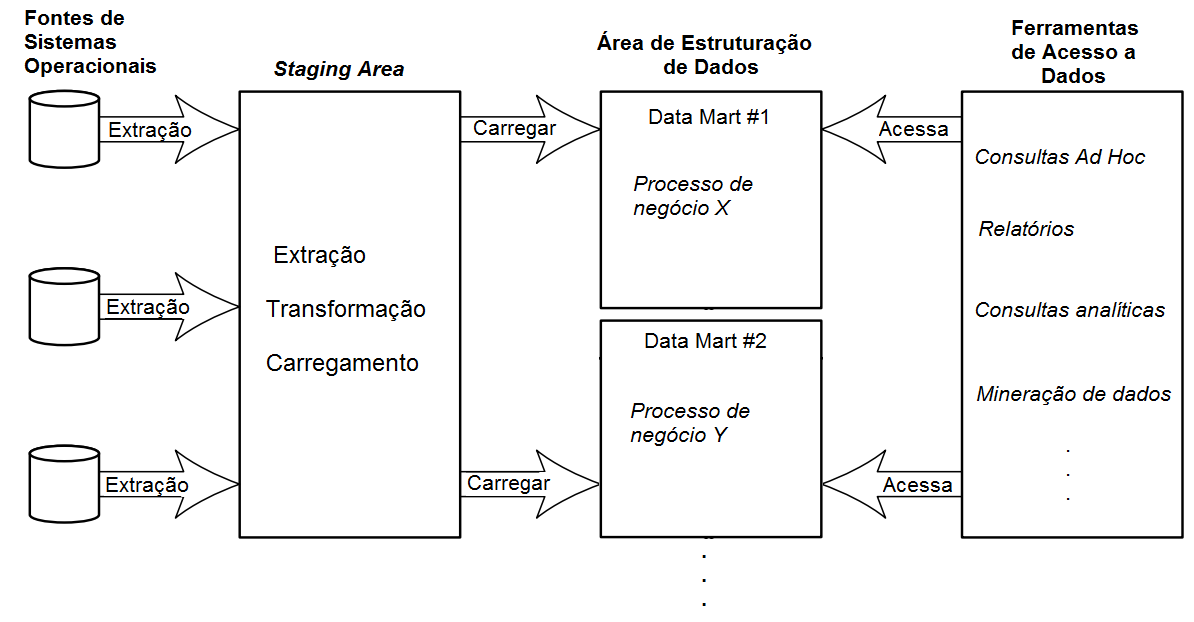
\includegraphics[width=\textwidth]{img/dw_arc}
	\caption{Arquitetura de um \textit{Data Warehouse}.}
	\label{fig:dw_arq}
\end{figure*}

Existe uma discussão acerca da modelagem conceitual da área de apresentação de dados de um ambiente de análise nos DWs \cite{sen2005comparison}. Segundo Sen e Sinha \cite{sen2005comparison} as duas técnicas de modelagem mais utilizadas são a Entidade-Relacional (ER) e a Dimensional. A primeira segue o padrão de modelagem para ambientes OLTP, que traduz a modelagem ER para um esquema relacional em seguida normalizando-o geralmente até a Terceira Forma Normal (3NF) \cite{kimball2002dw}, normalmente utilizadas por banco de dados relacionais. O modelo Dimensional, ou multidimensional, por sua vez, evita atingir o mesmo nível de normalização da modelagem ER, e faz analogia a um cubo para representação de dados, uma vez que uma informação pode ser vista através de \textit{n} dimensões. 

O modelo dimensional é composto por tabelas denominadas Tabelas Fato e Tabelas Dimensão \cite{kimball2002dw}, e é conhecido comumente como modelo \textit{star join}, ou apenas \textit{star} \cite{sen2005comparison}, pelo seu formato lembrar o de uma estrela. A Tabela Fato é a principal tabela do modelo Dimensional, contemplando atributos responsáveis por determinar as regras e métricas de negócio, ou um fato. Em sua maioria são atributos numéricos, relacionados a quantidade, e aditivos, visto que uma consulta em um DW pode retornar até milhares de tuplas, tornando interessante o conhecimento de informações como o total de um atributo dada alguma questão de negócio. Atributos textuais não são definidos como um fato, na maioria das vezes descrevem algo e devem estar inseridos em Tabelas Dimensão pois há maior chance de estarem relacionados com os atributos dimensão. Outro ponto a se ater é a importância de se evitar incluir dados com zeros que não representam dados úteis, ou representando nada, pois a inclusão de dados sem significado sobrecarregariam o DW sem motivo.

As Tabelas Fato são auxiliadas pelas Tabelas Dimensão no que concerne à descrição textual das questões de negócio. É comum essas tabelas terem de 50 a 100 atributos, ou mais, pois a intenção das dimensões é descrever as regras de negócio. É nestas tabelas que são realizados os filtros de consulta. Por filtros entende-se agrupamentos, padrões e ordenações por exemplo. De forma a exemplificar, se fosse desejado buscar as vendas por nome de fornecedor em um determinado intervalo de data, os atributos "nome de fornecedor" e "data" deveriam estar armazenados em tabelas dimensão. Segundo Kimball \cite{kimball2002dw}, quanto mais bem descritos os atributos dimensão, melhor o DW é, tornando a qualidade do \textit{warehouse} dependente das entidades de dimensão.

Todas as Tabelas Fato tem duas ou mais chaves relacionando-as às Tabelas Dimensão, como mostra o exemplo da Figura \ref{fig:star_dim}, onde a tabela \textit{Vendas} corresponde à uma Tabela Fato e as demais à Tabelas Dimensão. Note que esta figura também faz referência a um modelo \textit{star}.

\begin{figure*}[htpb]
	\centering
		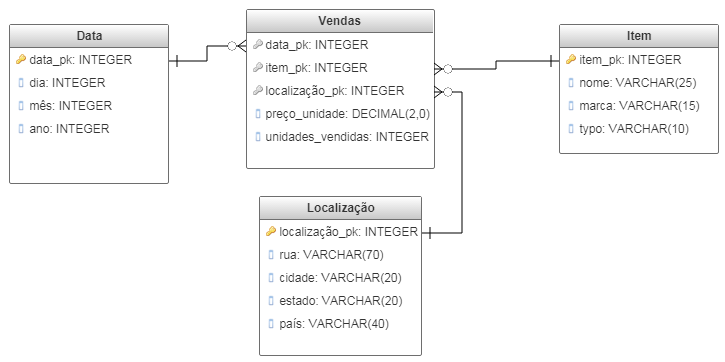
\includegraphics[width=13cm]{img/star_dim}
	\caption{Exemplo de esquema \textit{star} com tabelas Fato e Dimensão}
	\label{fig:star_dim}
\end{figure*}

Mesmo que a modelagem Dimensional não atinja a normalização 3NF, modelos \textit{star} podem ser trabalhados de forma a oferecer suporte à hierarquia de atributos às Tabelas Dimensão, permitindo que estas tenham Tabelas "Subdimensão". A esse refinamento se dá o nome de \textit{snowflake} \cite{navathe2011banco}. Embora tenham uma estrutura mais simplificada, segundo Levene e Loizou \cite{levene2003snowflake} a escolha do uso de esquemas \textit{snowflake} se dá por serem um esquema intuitivo, de fácil entendimento, passíveis à otimização de consultas, e de fácil extensão -- uma vez que pode-se adicionar atributos às tabelas sem interferir em programas já existentes. Uma possível adaptação de um modelo \textit{star} para \textit{snowflake} é como mostrado na Figura \ref{fig:snow}, no qual foi adaptado o modelo da Figura \ref{fig:star_dim}, adicionando a Tabela Subdimensão Cidade. 

\begin{figure*}[htpb]
	\centering
		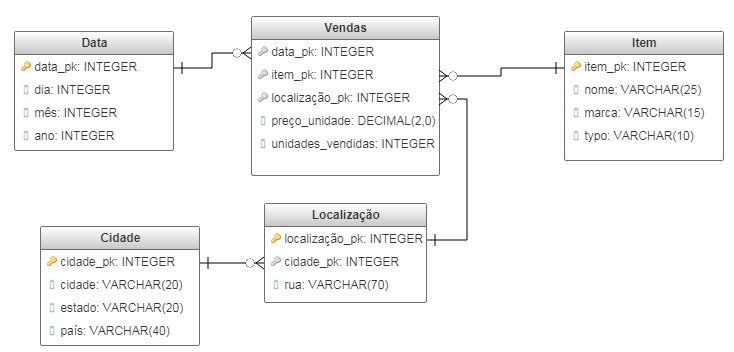
\includegraphics[width=13cm]{img/snow}
	\caption{Exemplo de esquema \textit{snowflake} adaptado da Figura \ref{fig:star_dim}}
	\label{fig:snow}
\end{figure*}

Para que possa ser construído um DW e aplicadas as modelagens acima descritas, 
é necessário alguma ferramenta que possa fazer o gerenciamento dele. 
De acordo com Elmasri e Navathe \cite{navathe2011banco} um banco de dados pode ser gerenciado por sistemas que 
facilitem este processo de gerenciamento no banco de dados. Estes sistemas são conhecidos como Sistemas Gerenciadores de Banco de Dados, ou SGBD.
% \graphicspath{ {3-SGBD/} }

\chapter{Sistemas Gerenciadores de Banco de Dados}
\label{sgbd}

Antes de se ter um sistema que visava gerenciamento de um banco de dados, era utilizado para persistência de dados o sistema de arquivos. 
Apesar de simples, esta abordagem apresentava alguns problemas por não apresentar suporte à redundância de informações; não garantir integridade de dados; 
falta de segurança; e o acesso e gerenciamento dos dados dependia de programas e aplicativos, fazendo com que seja necessário criar um novo aplicativo, ou adaptá-lo, a 
cada requisição de dados diferente. Outro problema crítico é não se ter informação de relacionamento entre arquivos diferentes.

Como forma de manter o gerenciamento de dados independente de aplicações e programas bem como solucionar os demais falhas do sistema de arquivos 
foram criados os Sistemas Gerenciadores de Bancos de Dados, os SGBD.  De acordo com Elmasri e Navathe \cite{navathe2011banco}, SGBD são uma coleção de programas para 
criação e manutenção de um banco de dados, que facilita a definição, construção, manipulação e compartilhamento de dados entre usuários e aplicações.

Dentre as vantagens que os SGBD trouxeram em detrimento ao sistema de arquivos estão:

\begin{itemize}
    \item{\textbf{Controle de redundância}}, para que não seja permitido duplicação de dados, pois isto causaria desperdício na capacidade de armazenamento.
    \item{\textbf{Restrição de acesso aos usuários}}, pois não será permitida manipulação do banco a todos os usuários, ou funcionários de uma empresa por exemplo.
    \item{\textbf{Execução de consultas eficiente}} através do uso de índices, normalmente implementadas utilizando hash ou árvores, para que o acesso ao disco seja mais rápido.
    \item{\textbf{Restrições de integridade}}, a fim de garantir que (i) dados não sejam inseridos de forma inconsistente de acordo com o tipo de atributo definido; 
    (ii) as relações entre entidades sejam efetuadas e (iii) restrições de chave sejam mantidas.
    \item{\textbf{Persistência de dados}}, para garantir que os dados serão inseridos e de fato armazenados no modelo.
    \item{\textbf{\textit{Backup}}} de dados periodicamente para evitar problemas caso aconteça alguma perda no banco e posterior \textbf{restauração}, para recuperar uma imagem do último backup feito no banco.
\end{itemize}

Existem várias classes de SGBD, conforme sua estruturação e a forma como manipulam os dados, 
entre as mais conhecidas estão o modelo relacional, objeto-relacional, orientado a 
objetos e a abordagem mais recente NoSQL.

\section{SGBD Relacional}

O modelo mais utilizado de SGBD é o relacional, ou SGBDR (SGBD Relacional). Ele foi conceituado por 
Codd \cite{codd1970relational} em 1970 em um artigo no qual são expostas as 
vantagens de um modelo relacional em detrimento a um modelo de redes. 

Um modelo relacional define através de um conjunto de tabelas entidades que representam 
objetos do mundo real, cada qual com seus atributos. Esse conjunto de atributos é 
denominado registro do banco de dados, representando uma tupla, ou linha, na tabela. Assim como no mundo real, 
objetos devem estar também relacionados, e para tal SGBDR utilizam-se de chaves.

Em um SGBDR além de definir relacionamentos, as chaves também garantem integridade entre os dados. 
Existem dois tipos de chaves, uma que garante a unicidade de um atributo, ou seja, assegura que 
não haverão registros repetidos no banco tomando como referência aquele valor de chave, chamada de chave primária (\textit{primary key}, ou PK). A outra chave garante integridade no relacionamento entre duas entidades referenciando uma tabela na outra, que 
é a chave estrangeira (\textit{foreign key}, ou FK).

Tomando como exemplo uma empresa fictícia, são criados dois objetos reais que precisam ser 
representados sob a forma relacional, \textit{funcionário} e \textit{projeto}. Nesta empresa funcionários possuem \textit{nome, 
CPF, sexo, salário,} um \textit{supervisor} e trabalham em um ou mais \textit{projetos}. Esses projetos também possuem atributos: 
\textit{nome, código} e o número do \textit{departamento} no qual foram criados. Apenas com estas informações duas tabelas já são definidas 
no banco, \textit{funcionário} e \textit{projeto}, bem como seus atributos, como ilustra a Figura \ref{fig:func_proj}.

\begin{figure*}[htpb]
	\centering
		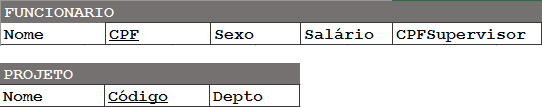
\includegraphics[width=13cm]{funcionario_projeto}
	\caption{Atributos das entidades \textit{funcionário} e \textit{projeto}}
	\label{fig:func_proj}
\end{figure*}

Como descrito, um funcionário trabalha em um ou mais projetos e ele precisa ainda registrar o número 
de horas trabalhadas nestes projetos. Desta forma é preciso de alguma forma relacionar funcionário com os projetos. 
Neste exemplo cabe a criação de uma nova entidade responsável unicamente por relacionar estes dois objetos e ainda 
armazenar o número de horas -- veja que o número de horas não cabe na tabela de funcionários nem na de projetos.

É nesta relação que são explorados os conceitos de chaves em um banco de dados. Para que a entidade que relaciona 
funcionário e projeto tenha informações de que funcionário trabalha em qual projeto é necessário acessar um número, ou código, 
definido para diferenciar todos os funcionários da empresa bem como o código do projeto e relacioná-los. Para o funcionário 
uma PK válida é o número do CPF e para o projeto o próprio atributo código. Essa relação pode ser nomeada unindo 
as entidades que relaciona, nesse caso \textit{funcionário\_projeto}, ou quando faz sentido pode ser nomeada de acordo com a função 
que realiza, neste caso como um funcionário trabalha em um projeto a relação pode ser \textit{trabalha\_em}.

O esquema que representa estas relações é como mostrado na Figura \ref{fig:relacao_func_proj}. Nela podemos ver as chaves primárias, em destaque, nas relações \textit{funcionário} e \textit{projeto}, e seus valores como chave estrangeira na relação \textit{trabalha\_em}. 

\begin{figure*}[htpb]
	\centering
		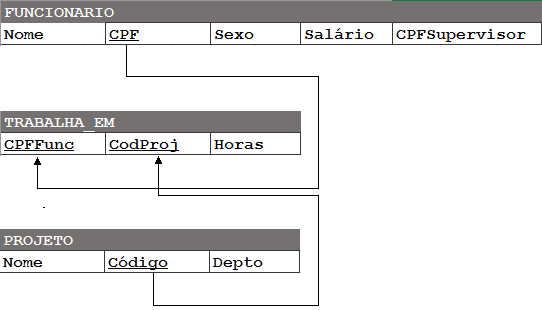
\includegraphics[width=13cm]{relacao_func_proj}
	\caption{Relacionamento entre \textit{funcionário} e \textit{projeto}}
	\label{fig:relacao_func_proj}
\end{figure*}

Modelos de bancos de dados prezam, sempre que possível, pela consistência de dados, principalmente se tomar operações transacionais como transações bancárias, que necessitam de um alto grau de consistência após operações de inserção e atualização, para que não haja perda de valores ou que esses ainda façam sentido no sistema. Por essa razão SGBDR seguem o conceito ACID (Atomicidade, Consistência, Isolamento e Durabilidade). 

Modelos relacionais também seguem um alto grau de normalização nos dados a fim de evitar redundância e confusão entre atributos que podem ser desmembrados em outras entidades. Essa normalização é realizada normalmente até a Terceira Forma Normal (3NF), e o esquema final conterá um número maior de tabelas que o original devido ao desmembramento de atributos. Essa quantidade maior de tabelas acarreta no aumento de junções necessárias para recuperar atributos entre entidades relacionadas, ou seja, no aumento do acesso a entidades e no processamento de tuplas.

Além de diminuir o desempenho na recuperação de dados, um esquema normalizado causa um forte acoplamento entre tabelas, o que tornaria inviável o particionamento dos dados do banco em \textit{n} servidores como forma de escalar estes dados conforme seu volume aumenta (mais detalhes no Capítulo \ref{nosql}), como é o caso de um ambiente analítico. Uma solução trivial para este problema é a denormalização de dados, porém para um SGBDR essa solução pode não ser viável, visto que sua implementação se dá seguindo a modelagem relacional.

Exemplos de SGBDR são PostgreSQL \cite{postgres2018r}, MySQL \cite{mysql2018r}, Microsoft SQL Server \cite{microsoft2018r}, SQLite \cite{lite2018r}, MariaDB \cite{maria2018r} e Oracle \cite{oracle2018r}. 

\section{SGBD NoSQL}

Bancos com o objetivo de suprir problemas apresentados por SGBDR começaram a emergir entre 2004 e 2007 visando alta escalabilidade, recuperação e armazenamento de grandes volumes de dados de forma eficiente, e ao mesmo tempo diminuir custos com hardware \cite{han2011nosql}. Esses bancos levaram o nome de NoSQL, porém isso não significa que não utilizam SQL para manipulação de dados.

Detalhes sobre bancos de dados NoSQL são encontrados no Capítulo \ref{nosql}, no qual também é descrito o modelo colunar, utilizado por satisfazer os requerimentos de um ambiente de DW.
% \graphicspath{ {4-NoSQL/} }
\chapter{NoSQL}
\label{nosql}

O desenvolvimento de novas aplicações e surgimento de novas soluções 
para sistemas gerou crescimento no volume de dados de maneira acelerada. 
Com isso cresce também o número de usuários, necessitando portanto escalar 
o BD. Existem duas soluções para escalar um sistema: o 
escalonamento vertical, que consiste em um \textit{upgrade} do servidor no 
qual o banco está hospedado; e o horizontal, aumentando o número de 
servidores e distribuindo o banco \cite{pritchett2008base, sharding2018educative}. 

Existem algumas desvantagens no \textit{upgrade} de um sistema. 
O BD pode superar a capacidade da melhor configuração 
disponível no mercado, e ainda é caro por requerer a aquisição de 
uma configuração melhor. Mesmo considerado mais complexo, o 
escalonamento horizontal é mais viável. Entre as soluções apresentadas 
no particionamento horizontal estão o particionamento funcional e o 
\textit{sharding} \cite{pritchett2008base}. 

O particionamento funcional consiste em fragmentar os dados de acordo 
com a forma como são utilizados dado um contexto. Um esquema com quatro entidades, 
\textit{usuários}, \textit{produtos}, \textit{clientes} e \textit{endereço} 
pode ser distribuído em quatro servidores, 
um para cada entidade. Entidades que são utilizadas somente para leitura podem 
ser separadas de entidades onde dados são escritos, caracterizando outro 
exemplo de particionamento funcional. O problema com esta estratégia está 
no acoplamento entre entidades: se duas ou mais entidades estiverem 
relacionadas elas deverão estar no mesmo servidor, caso contrário não 
será possível atribuir as restrições de chave àquele relacionamento \cite{pritchett2008base}. 
Tomando o exemplo acima com as quatro entidades, supondo que \textit{cliente} 
e \textit{endereço} estejam relacionadas estas devem 
ser armazenados no mesmo servidor. 

A segunda estratégia, o \textit{sharding}, consiste em dividir os dados do banco 
utilizando algum critério de separação de dados que não seja limitado à 
funcionalidade das entidades. Soluções como particionamento com base em 
\textit{hash} ou listas podem ser aplicadas. Considerando dez servidores e uma chave 
primária auto-incremental, a função de \textit{hash} pode tomar o módulo da chave 
primária pelo total de servidores como critério de seleção da partição 
na qual o dado será inserido. Utilizando uma lista é possível definir valores 
para os servidores e distribuir os dados de acordo com esses valores. 
Por exemplo, as linguagens C++, Java e C\# poderiam ser inseridas em uma 
partição destinada à linguagens orientadas a objeto.

O \textit{sharding} enfrenta problemas com junções entre dados, visto que os dados 
devem ser recuperados de diferentes partições e a maioria dos SGBDR não 
oferece suporte a chaves estrangeiras sob diferentes servidores, restando 
ao desenvolvedor tratar isso no código da aplicação \cite{pritchett2008base}. 
Uma solução para tais 
problemas é a denormalização de dados para que o número de junções diminua ou, 
no melhor dos casos e quando possível, seja zero. Contudo, isso é um problema 
para modelos relacionais, visto que trabalham sobre uma modelagem normalizada de dados. 
Além disso e de não se adaptarem à escalabilidade horizontal, 
são complexos e o fato de trazerem todas as informações de uma entidade sob a 
forma de tuplas causa lentidão em um ambiente analítico na recuperação de dados, 
cujas consultas percorrem o banco visando atributos específicos, processando 
somente o necessário. 

Outro problema crítico ao não utilizar a escalabilidade horizontal está na 
disponibilidade dos dados. Enquanto um banco se apoiar na escalabilidade vertical, 
qualquer queda no servidor acarretará na queda total no sistema de armazenamento, 
ao passo que quando se trabalha com servidores em paralelo a queda em uma máquina 
não trará prejuízos no conjunto todo. Assim, soluções como melhorar o hardware do 
servidor continuam sendo desvantajosas. Além da escalabilidade, disponibilidade 
de dados foi um dos argumentos utilizados por um dos engenheiros da rede social 
Twitter ao migrar do MySQL para o Cassandra, um SGBD NoSQL. 
Em 2008 a rede ficou fora do ar por 84h \cite{twitter2010}.

Com o intuito de suprir tais problemas de escalabilidade, disponibilidade 
e recuperação rápida de dados, entre 2004 e 2007 os SGBD NoSQL começaram 
a ganhar destaque com o surgimento das bases de dados BigTable da Google \cite{chang2008bigtable}, e Dynamo 
da Amazon \cite{decandia2007dynamo}. O termo NoSQL, embora a princípio pareça indicar total independência 
de SQL, significa \textit{Not Only SQL}, “Não Apenas SQL”. Também, ele não descreve um 
único tipo de SGBD, mas sim uma classe de modelos, cada qual com suas propriedades. 
As mais conhecidas são quatro:

\begin{itemize}
    \item{\textbf{Orientado a Grafos}}, que se utiliza da Teoria dos Grafos para estruturar seus dados. 
    Um exemplo desta classe é o Neo4j \cite{neo2018nosql}.
    \item{\textbf{Orientado a Chave-Valor}}, que armazena os dados de forma similar a uma tabela \textit{hash}, 
    com uma chave referenciando um valor, ou tipo de dado. Exemplos são o Project Voldemort \cite{voldemort2018nosql}, 
    DyanmoDB \cite{amazon2018nosql}, o Riak \cite{riak2018nosql} e o Redis \cite{redis2018nosql}.
    \item{\textbf{Orientado a Documento}}, uma versão melhorada do Chave-Valor, 
    no qual os valores são armazenados como documentos através de estruturas complexas como JSON e XML. 
    Exemplos são o MongoDB \cite{mongo2018nosql} e o CouchDB \cite{couch2018nosql}.
    \item{\textbf{Orientado a Colunas}}, ou modelo colunar, 
    que utiliza tabelas como armazenamento de entidades, 
    porém não agrupa os dados sob forma de tuplas, e sim colunas. Exemplos são o MonetDB \cite{monetdb2017c}, C-Store \cite{cstore2018nosql}, BigTable \cite{google2018nosql} e Cassandra \cite{cassandra2018nosql}.
\end{itemize}

De maneira geral, as vantagens no uso de um SGBD NoSQL estão no rápido processamento de um grande volume de dados, flexibilidade para expansão e baixo custo de escalabilidade. Devido ao vasto número de SGBD dentro de cada classe de NoSQL, esses bancos também podem ser classificados de acordo com o Teorema CAP (do inglês \textit{Consistency, Availability, Partition tolerance}). Segundo Eric Brewer \cite{brewer2000towards, gilbert2002brewer}, um sistema distribuído não é 
capaz de conciliar consistência, disponibilidade e tolerância a partição de dados simultaneamente, tendo que optar por apenas dois destes. 
SGBDR prezam por disponibilidade e consistência de dados seguindo o ACID, porém a preocupação com consistência 
pode tornar a manipulação de dados lenta. Visto que o movimento NoSQL surgiu com a intenção de 
melhorar a escalabilidade e disponibilidade de dados, e tornar a manipulação destes mais rápida, 
a maioria deles trabalha com os atributos de disponibilidade e tolerância à partição. 
Essa configuração assume um conceito diferente do ACID para bancos NoSQL, e Pritchett \cite{pritchett2008base} propôs um teorema diferente do ACID, mais otimista, onde a consistência é relaxada, o Teorema BASE (\textit{Basically Available, Soft State, Eventual Consistency}).

O Teorema BASE assume que a consistência em um banco 
de dados está em estado de fluxo, ao contrário do ACID que força a consistência a cada operação, 
sendo este considerado pelo autor um método pessimista. 
Neste cenário a disponibilidade é garantida devido à tolerância a partição, fazendo 
com que a falha de um servidor não cesse o funcionamento de todo o sistema -- por exemplo, caso uma partição falhe em um sistema rodando sobre dez servidores, apenas 10\% dos dados estarão indisponíveis e somente os usuários daquela partição serão afetados.


\section{SGBD Colunar}

Dentre as categorias de bancos de dados NoSQL a que melhor se adequa aos 
propósitos analíticos é a colunar. Sistemas colunares armazenam seus dados 
em colunas que representam atributos das entidades, fazendo com que apenas os atributos necessários sejam 
lidos \cite{khoshafian1987query}, o que diminui o tempo de acesso 
ao disco \cite{matei2010column, abadi2008column}. Cada uma destas colunas pode armazenar seus valores utilizando o par 
\textit{chave, valor} \cite{abadi2013design, khoshafian1987query}, sendo esta uma das formas de implementação 
de um sistema colunar (descrita na Seção \ref{sec:implementacao_col} deste capítulo). 
A Figura X ilustra de forma simples, embora apenas visual, 
a diferença principal entre um armazenamento utilizando linhas e outro utilizando 
colunas.

Matei \cite{matei2010column} cita algumas vantagens de sistemas colunares:

\begin{itemize}

    \item{\textbf{Melhor desempenho}}, pela forma com que os dados são armazenados e o uso de índices 
    visando o armazenamento ao invés de localização de registros, resultando em menos operações de 
    entrada e saída.
    \item{\textbf{Rápidas operações de agrupamento}}, bastante utilizadas em ambientes OLAP, visto 
    que valores de um mesmo atributo são armazenados consecutivamente. Bem como operações matemáticas, 
    como recuperar o maior ou menor valor, soma e média.
    \item{\textbf{Alta compressão de dados}} pode ser alcançada, devido às chances de se ter 
    valores repetidos para um mesmo atributo serem maiores.

\end{itemize}

Existem diferentes abordagens para se implementar um SGBD colunar. Essas abordagens levam em conta 
mudanças na codificação de um banco, apenas na modelagem dele, bem como se será possível atingir 
níveis altos de compressão. A primeira técnica consiste no \textbf{particionamento vertical} dos dados, a 
segunda em \textbf{modificar a camada de armazenamento} e a terceira corresponde a junção de ambas.

\section{Implementação do Sistema Colunar}
\label{sec:implementacao_col}

Antes de detalhar os métodos de implementação de um BD colunar, é fundamental discutir sobre a reconstrução de tuplas nesse tipo de SGBD. 
Segundo Abadi et al. \cite{abadi2007materialization}, a parte lógica e visual de um BD colunar se apresenta da mesma forma que 
um BD relacional. Isso faz com que a maioria dos SGBD colunares ofereçam uma interface relacional de comunicação, compatível com os padrões.

Como os atributos de um modelo colunar acabam ficando separados em disco um do outro, eles precisam ser unidos novamente em tuplas para 
que o resultado de uma consulta seja exibido. Existem duas técnicas para realizar essa reconstrução, ou materialização: \textit{early materialization} (EM) e 
\textit{late materialization} (LM) \cite{abadi2007materialization, abadi2008query}.

A \textit{early materialization}, melhor traduzida como materialização prévia nesse contexto, é a política adotada por BD relacionais, e consiste 
em adicionar as colunas à tupla conforme a coluna é requisitada na consulta. Essa técnica não leva em conta o predicado da consulta, isto é, considere 
a consulta a seguir:

\begin{lstlisting}[language=SQL,label=sql_1]
                    SELECT nome FROM funcionario 
                    WHERE salario >= 1000 AND sexo='F'
\end{lstlisting}

A EM irá processar essa consulta e construir uma tupla com os atributos \textit{nome, salário} e \textit{sexo}, com todos os registros 
armazenados em banco. Considere que os registros são como mostrados na Figura X. Esse método só analisa o predicado após a construção das tuplas. Isso não acontece na LM. 

% inserir imagem com valores de registros

Na LM, ou materialização tardia, é analisado primeiro o predicado e verificado quais valores atendem a esse predicado em cada coluna. 
No caso da SQL acima primeiro seria analisado o predicado de seleção, nesse caso \texttt{WHERE salario >= 1000 AND sexo='F'}, e então 
através de um operador lógico AND seria possível retornar a posição dos atributos que satisfazem essa seleção, para então 
construir a tupla a partir do predicado de projeção somente com o atributo \textit{nome}. Em suma, apenas após ter a posição de cada atributo é que a tupla é construída, descartando a reconstrução de tuplas que seriam posteriormente descartadas. A Figura A e B representam o resultado final de cada materialização.

% inserir subfigure com tuplas

\subsection{Particionamento Vertical}

Considerada a técnica mais simples para implementar um banco colunar, esta técnica 
realiza a partição dos dados de forma que cada atributo de uma entidade seja armazenado 
em uma tabela de duas colunas contendo o par <chave/índice, valor do atributo> \cite{khoshafian1987query}.

% inserir figura de particionamento vertical

A Figura Y mostra que é possível desmembrar o esquema relacional em colunas de atributos. 
No momento em que uma consulta analítica é realizada, não serão processados dados além 
dos de fato requeridos e nenhum dado é perdido pois ainda haverá referência entre os atributos 
através das chaves.

Essa abordagem é a mais simples de se implementar, pois nenhuma mudança é feita 
na codificação do BD, sendo que a única alteração necessária está a nível 
da aplicação responsável por executar as consultas, mudando a lógica de acesso aos dados. Isso torna prático para empresas a 
mudança entre a estratégia relacional e a colunar, pois torna possível o uso de um mesmo 
SGBD como DW.

Ao mesmo tempo que essa implementação traz praticidade na migração de dados, ela não difere 
muito da abordagem relacional no que concerne ao desempenho. Em Abadi \cite{abadi2008query} 
é mostrado que adaptar dados de um esquema relacional utilizando particionamento vertical não 
trouxe melhoras no desempenho das consultas. Foi verificado que o custo de junções para unir 
as colunas é alto conforme a quantidade de atributos selecionados aumenta e não foi possível 
usufruir eficientemente da compressão de dados.

\subsection{Modificação na Camada de Armazenamento}

A segunda abordagem para implementar um sistema colunar consiste em já modificar o armazenamento do banco. Essa técnica não altera a parte 
lógica da modelagem do banco, mas a camada física alterando o armazenamento de 
linha por linha para coluna por coluna. Nessa implementação as chaves não precisam ser 
repetidas como na abordagem anterior, na qual a primeira coluna de cada tabela 
consistia no valor de chave da cada atributo. O \textit{i-ésimo} valor de atributo 
de uma coluna estará associado ao \textit{i-ésimo} atributo das demais colunas e 
não é desperdiçado espaço em disco com as chaves.

Neste método a reconstrução de tuplas é realizada antes da execução da consulta de fato. Como apenas um determinado número de atributos precisa ser acessado, estes são combinados seguindo a lógica que o \textit{i-ésimo} atributo de uma coluna está relacionado com o \textit{i-ésimo} atributo das demais. Aqui tem-se uma vantagem no modelo orientado a linhas, por este já armazenar as sob o formato de linhas e não precisar armazenar os dados em ordem.

\subsection{Modificação na Camada de Armazenamento e Particionamento Vertical}

A última, e melhor, abordagem consiste em modificar a camada de armazenamento do BD e a aplicação que processa as consultas \cite{stonebraker2005c, boncz2005monetdb}, assim o processador pode manter os dados sob a forma de colunas sem precisar unir as colunas e construir tuplas. Uma vantagem óbvia desta técnica é a eliminação da reconstrução de tuplas e com isso menos dados precisam ser previamente movimentados, diminuindo 
o tempo de processamento.  

\section{Compressão de Dados}

Uma característica marcante de um SGBD colunar é a alta possibilidade de compressão de dados. 
Existem diversas formas de comprimir os dados, porém deve-se ater ao fato de 
que o tempo de compressão e descompressão não deve afetar significativamente o processamento 
dos dados no SGBD. Para tal, uma solução é utilizar métodos que consigam operar sob os dados 
ainda comprimidos -- ainda nesta seção são apresentados alguns dos algoritmos utilizados para 
compressão em BD.

Como exemplo, apenas ilustrativo, de como os dados em um sistema colunar podem ser comprimidos de forma mais 
eficiente que em um relacional, considere a entidade \textit{usuário} a seguir, com os 
atributos \textit{id, nome, idade} e \textit{sexo}. A primeira coluna corresponde aos índices utilizados no banco. 

\begin{verbatim}
    1: 0, Bruno, 50, M
    2: 10, João, 23, M
    3: 20, Maria, 30, F
    4: 90, Ana, 23, F
    5: 78, Gabriel, 23, M
\end{verbatim}

Um banco relacional armazena estes atributos da forma como foram apresentados acima. 
Considerando o armazenamento colunar, os mesmos dados seriam armazenados da seguinte forma: 

\begin{verbatim}
    1: 0, 2: 10, 3: 20, 4: 90, 5: 78
    1: Bruno, 2: João, 3: Maria, 4: Ana, 5: Gabriel
    1: 50, 2: 23, 3: 30, 4: 23, 5: 23
    1: M, 2: M, 3: F, 4: F, 5: M
\end{verbatim}

Note que fica mais claro que como os atributos são armazenados em uma coluna com chave e valor 
existirão mais chances de repetição de valores em uma mesma coluna. Os atributos \textit{idade} e 
\textit{sexo} se repetem para alguns registros, possibilitando assim compressão destes dados. 
Comprimindo estas repetições o nosso modelo é armazenado da forma: 

\begin{verbatim}
    1: 0, 2: 10, 3: 20, 4: 90, 5: 78
    1: Bruno, 2: João, 3: Maria, 4: Ana, 5: Gabriel
    1: 50, 2, 4, 5: 23, 3: 30
    1, 2, 5: M, 3, 4: F
\end{verbatim}

Westmann et al. \cite{westmann2000implementation} consideram que os métodos de compressão em um BD devem ser capazes de se aplicar 
no banco como um todo, bem como em uma tupla ou a cada atributo de tupla, e serem rápidos em processamento quando há casos em que seja 
necessário realizar descompressão.

O primeiro método consiste em comprimir a representação de valores inteiros, baseado no algoritmo \textit{null supression} \cite{westmann2000implementation, roth1993database}. A ideia é descartar zeros na representação de um inteiro de quatro bytes, por exemplo, 
ao invés de se representar o número 10 da forma '00000000000000000000000000001010', seriam utilizados apenas quatro bits, '1010'. É 
necessário entretanto guardar a informação de quantos bits são utilizados para armazenar um número e em alguns casos também é preciso 
armazenar um bit a mais para o sinal do inteiro. Esse algoritmo pode ser utilizado para comprimir o tamanho de strings no banco 
quando estas são representadas pelo tipo VARCHAR, visto que para esse tipo de dado o tamanho também é armazenado devido a possibilidade 
deste variar.

Um método bastante empregado é a Codificação por Dicionário. Nele atributos que possuem um padrão fixo, por exemplo, os números primos de 
3 a 19 (3, 5, 7, 11, 13, 17, 19), podem ser representados por um dicionário de 3 bits. Este algoritmo pode ser utilizado para compressão 
de valores NULL, considerando-o como um possível valor no padrão.

Abadi, Madden e Ferreira \cite{abadi2006integrating} utilizam a compressão por dicionário e uma variação do algoritmo \textit{null supression} para implementar o BD C-Store e ainda apresentam dois outros métodos. O primeiro é o \textit{run-length}, que pode ser bem aproveitado 
em bancos colunares quando atributos são repetidos sequencialmente e possuem pouca variação. Ele consiste em contar o número de vezes no qual 
um valor é repetido utilizando a tripla (valor, posição inicial, tamanho). Um exemplo é ilustrado na Figura A com o atributo \textit{especialização}.

% inserir uma imagem run length com graduação, mestrado, doutorado.

O último método apresentado pelos autores é a Codificação por Vetor de Bit, bastante útil quando uma coluna possui número limitado 
de possibilidades, como linguagens de programação dentro de um dado paradigma ou estados do Brasil. Uma string de bits representa a 
ocorrência do valor de atributo, onde '1' representa a ocorrência naquela posição e '0' a não ocorrência. Como exemplo, uma coluna com os 
valores {M M F M F F M} podem ser representados pela cadeia de bits 1 1 0 1 0 0 1 para o valor M, e 0 0 1 0 1 1 0 para F.

Em suma, ao implementar um banco colunar tanto a aplicação deve ser capaz de entender e conseguir recuperar informações mesmo comprimidas, como a modificação da camada de armazenamento deve ser implementada tal que se possa usufruir de algum método de compressão. Caso contrário um 
dos principais diferenciais de modelos colunares não será explorado e poderá não haver impacto no desempenho quando trabalhado com uma 
grande massa de dados, como é a realidade de empresas.

\graphicspath{ {3-FUNDAMENTOS/} }

\chapter{Fundamentação Teórica}
\label{sgbd}

Um ativo importante em qualquer organização é a informação. Segundo Kimball e Ross \cite{kimball2002dw} essa informação é mantida sob duas formas: sistemas de banco de dados operacionais e \textit{Data Warehouses}. Em sistemas operacionais geralmente os usuários lidam com o mesmo registro e realizam a mesma tarefa exaustivamente sob uma única informação, permanecendo no domínio das transações; enquanto que em um DW pode-se ver o progresso da organização utilizando dados armazenados continuamente, de forma otimizada para a recuperação de dados. Também, são formuladas perguntas com a finalidade de responder a alguma questão de negócio, como \textit{"quantos pedidos foram recebidos pelo fornecedor X no período de tempo Y?"}, ou \textit{"qual foi o impacto no número de vendas ao mudar o formato de envio de A para B?"}. Para responder questões dessa natureza não é viável lidar com dados de forma individual, mas sim recuperar um conjunto de dados a fim de formular uma resposta.

De acordo com Inmon \cite{inmon2005building}, DWs são base de todos os Sistemas de Suporte à Decisão (do inglês \textit{Decision Support Systems}, ou DSS). DSS são tecnologias utilizadas para decisões de negócio e solução de problemas, 
e incluem componentes que realizam gerenciamento de banco de dados e que 
permitem uma interação com o usuário de forma a simplificar consultas e geração de relatórios 
\cite{shim2002past}. DWs foram as primeiras ferramentas a surgirem como solução para o 
suporte à decisão de negócio, integrando dados de diferentes bancos de dados operacionais 
\cite{inmon2005building, kimball2002dw}.

De forma geral, um DW é um repositório de dados capaz de fornecer rapidamente 
informações consistentes e cruciais para a tomada de decisão de uma organização, 
de tal forma que essa informação possa ser acessada de maneira intuitiva e legível 
pelo usuário, a fim de combinar diferentes informações entre os dados armazenados 
\cite{kimball2002dw}. Deve também se adaptar a possíveis mudanças, sejam elas mudanças comerciais, mudanças nos dados ou na tecnologia. Inmon \cite{inmon2005building} define um DW como "uma coleção de dados não-volátil, ou seja, que não muda após inserida no \textit{warehouse}; orientado ao assunto principal da organização; integrado e variante no tempo para que seja mantido um histórico a fim de analisar situações passadas". Do ponto de vista estrutural, Wremble e Koncilia \cite{wrembel2007data} definem um DW como uma base de dados homogênea, local e centralizada.

Para analisar os dados de um DW além de implementá-lo é necessário que alguma aplicação leia seu conteúdo e apresente-o de forma gráfica e intuitiva ao analisador. Aplicações OLTP (\textit{On-Line Transactional Processing}) são utilizadas por bancos de dados operacionais e operam transações atômicas e isoladas de forma repetitiva, que correspondem ao dia-a-dia de uma organização \cite{chaudhuri1997overview}. DWs trabalham com suporte à decisão e são intensivos à consultas \textit{ad hoc} complexas, que acessam milhões de registros. Sendo assim, os dados históricos, a taxa de vazão de uma consulta e o tempo de resposta são mais importantes que pequenas transações.

À aplicação aceita por um DW dá-se o nome de OLAP, cujo objetivo, de acordo com Codd; Codd e Salley \cite{codd1998providing}, é identificar tendências, padrões de comportamento e anomalias, bem como relações em dados aparentemente não relacionados. Geralmente as consultas em uma aplicação analítica são longas, levam tempo para executar e estão interessadas 
em atributos específicos. Os resultados dessas análises servem de base para tomada de decisões de negócio. Ainda, o processo de inserção de dados em um ambiente OLAP é um pouco mais complexo que sistemas OLTP por seguir um processo fim-a-fim conhecido 
como ETL (extração, transformação e carga, do inglês \textit{extract, transformation, load}) \cite{vertabelo2017olap}. Portanto, DWs e aplicações OLAP são componentes chave para a construção de um ambiente de análise.

O processo ETL faz parte da arquitetura de um DW. Neste domínio existem diversos componentes que realizam funções específicas a fim de construir um ambiente de \textit{warehouse} desde a obtenção dos dados de fontes externas e sistemas operacionais de bancos de dados, até o acesso a esses dados por meio do DW por alguma consulta analítica definida sob uma aplicação OLAP. Para entender esta arquitetura fim-a-fim, ilustrada na Figura \ref{fig:dw_arq} adaptada de Kimball e Ross \cite{kimball2002dw}, é necessário compreender alguns componentes e conceitos que formam um DW \cite{kimball2002dw}:

\begin{itemize}
    \item \textbf{Sistemas de Fonte Operacional}: possuem detalhes sobre as transações do negócio, correspondendo a ambientes OLTP. Engloba os dados que irão estruturar as informações do DW, portanto, se encontram externos ao \textit{warehouse}. Podem ser tanto sistemas de banco de dados ou alguma outra fonte de dados, como um documento no formato XLS, CSV, TXT; e sistemas CRM.
    \item \textbf{\textit{Staging Area}}: compreende tanto uma área de armazenamento temporária quanto um conjunto de processos denominado ETL. De forma geral é uma área a qual os usuários não têm acesso, onde os dados são traduzidos para algo que possa ser enviado de maneira compatível ao \textit{warehouse} e não se trabalha diretamente sobre os dados transacionais. Quanto aos processos ETL, a fase de Extração (\textit{Extraction}) consiste na leitura da fonte de dados, transferindo o conteúdo necessário para a \textit{staging area}; após essa extração pode ser necessário realizar uma "limpeza" nos dados; unir dados de diferentes fontes; tratar duplicatas e atribuir chaves do \textit{warehouse}. A isto dá-se o nome de Transformação (\textit{Transformation}). A última fase, fase de Carga (\textit{Load}), é responsável por carregar, ou popular, os dados na área de estruturação de dados do DW.
    \item \textbf{Estruturação de Dados}: trata de como os dados serão organizados, armazenados e disponibilizados para consultas de usuários, relatórios e outras aplicações. No que tange à comunidade empresarial, a fase de apresentação de dados \textit{é} o DW em si, pois corresponde ao que pode ser acessado via ferramentas de acesso a dados. A etapa de estruturação é comumente definida como sendo um conjunto de \textit{data marts}. \textit{Data marts} são subconjuntos do total de informações de um DW, cada qual representando os dados de um determinado assunto, departamento, ou processo de negócio. Nesta fase é definida a modelagem conceitual do ambiente de análise do DW.
    \item \textbf{Ferramentas de Acesso aos Dados}: são formas de aplicar uma consulta, dentro de aplicações OLAP, aos dados organizados na fase de estruturação. Pode ser uma consulta \textit{ad hoc} ou algo mais complexo, como consultas aplicadas à mineração de dados.
    
\end{itemize}

\begin{figure*}[htpb]
	\centering
		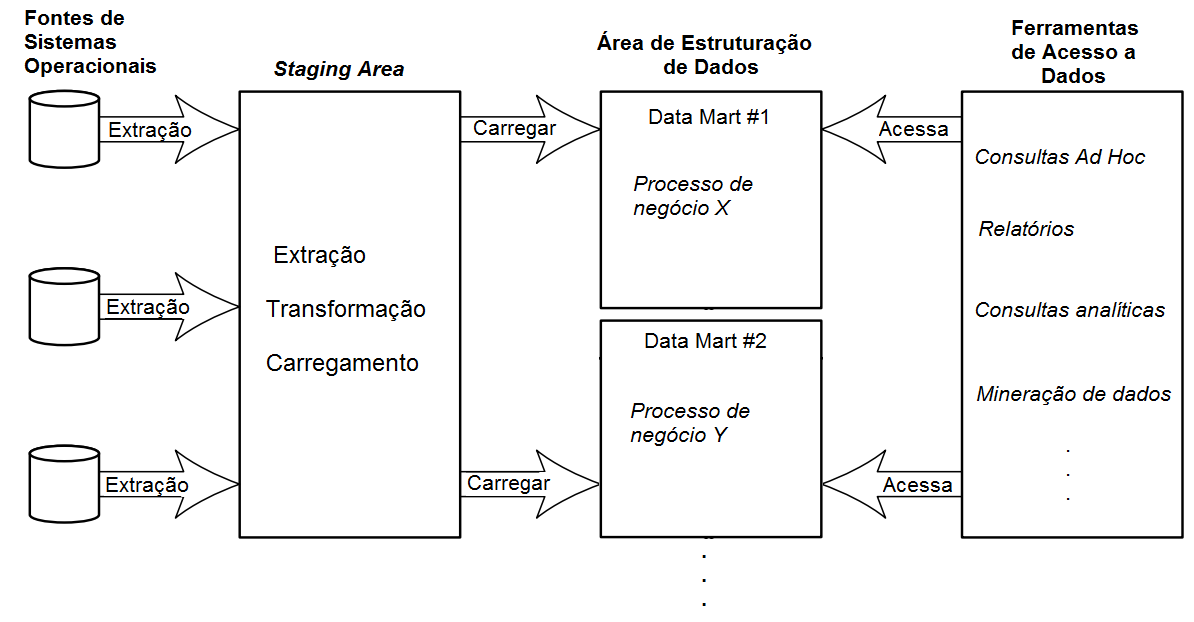
\includegraphics[width=\textwidth]{img/dw_arc}
    \caption[Arquitetura de um \textit{Data Warehouse}]
        {Arquitetura de um \textit{Data Warehouse} \\ Fonte: adaptado de Kimball e Ross \cite{kimball2002dw}}
	\label{fig:dw_arq}
\end{figure*}

Existe uma discussão acerca da modelagem conceitual da área de apresentação de dados de um ambiente de análise nos DWs \cite{sen2005comparison}. Segundo Sen e Sinha \cite{sen2005comparison} as duas técnicas de modelagem mais utilizadas são a Entidade-Relacional (ER) e a Dimensional. A primeira segue o padrão de modelagem para ambientes OLTP, que traduz a modelagem ER para um esquema relacional em seguida normalizando-o geralmente até a Terceira Forma Normal (3NF) \cite{kimball2002dw}, normalmente utilizadas por banco de dados relacionais. O modelo Dimensional, ou multidimensional, por sua vez, evita atingir o mesmo nível de normalização da modelagem ER, e faz analogia a um cubo para representação de dados, uma vez que uma informação pode ser vista através de \textit{n} dimensões. 

O modelo dimensional é composto por tabelas denominadas Tabelas Fato e Tabelas Dimensão \cite{kimball2002dw}, e é conhecido comumente como modelo \textit{star join}, ou apenas \textit{star} \cite{sen2005comparison}, pelo seu formato lembrar o de uma estrela. A Tabela Fato é a principal tabela do modelo Dimensional, contemplando atributos responsáveis por determinar as regras e métricas de negócio, ou um fato. Em sua maioria são atributos numéricos, relacionados a quantidade, e aditivos, visto que uma consulta em um DW pode retornar até milhares de tuplas, tornando interessante o conhecimento de informações como o total de um atributo dada alguma questão de negócio. Atributos textuais não são definidos como um fato, na maioria das vezes descrevem algo e devem estar inseridos em Tabelas Dimensão pois há maior chance de estarem relacionados com os atributos dimensão. Outro ponto a se ater é a importância de se evitar incluir dados com zeros que não representam dados úteis, ou representando nada, pois a inclusão de dados sem significado sobrecarregariam o DW sem motivo.

As Tabelas Fato são auxiliadas pelas Tabelas Dimensão no que concerne à descrição textual das questões de negócio. É comum essas tabelas terem de 50 a 100 atributos, ou mais, pois a intenção das dimensões é descrever as regras de negócio. É nestas tabelas que são realizados os filtros de consulta. Por filtros entende-se agrupamentos, padrões e ordenações por exemplo. De forma a exemplificar, se fosse desejado buscar as vendas por nome de fornecedor em um determinado intervalo de data, os atributos "nome de fornecedor" e "data" deveriam estar armazenados em tabelas dimensão. Segundo Kimball \cite{kimball2002dw}, quanto mais bem descritos os atributos dimensão, melhor o DW é, tornando a qualidade do \textit{warehouse} dependente das entidades de dimensão.

Todas as Tabelas Fato tem duas ou mais chaves relacionando-as às Tabelas Dimensão, como mostra o exemplo da Figura \ref{fig:star_dim}, onde a tabela \textit{Vendas} corresponde à uma Tabela Fato e as demais à Tabelas Dimensão. Note que esta figura também faz referência a um modelo \textit{star}.

\begin{figure*}[htpb]
	\centering
		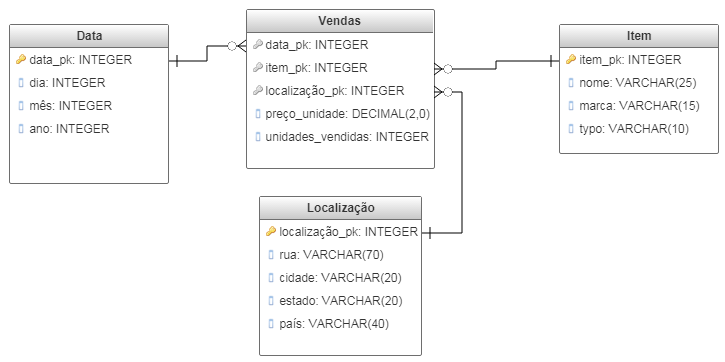
\includegraphics[width=13cm]{img/star_dim}
	\caption{Exemplo de esquema \textit{star} com tabelas Fato e Dimensão}
	\label{fig:star_dim}
\end{figure*}

Mesmo que a modelagem Dimensional não atinja a normalização 3NF, modelos \textit{star} podem ser trabalhados de forma a oferecer suporte à hierarquia de atributos às Tabelas Dimensão, permitindo que estas tenham Tabelas "Subdimensão". A esse refinamento se dá o nome de \textit{snowflake} \cite{navathe2011banco}. Embora tenham uma estrutura mais simplificada, segundo Levene e Loizou \cite{levene2003snowflake} a escolha do uso de esquemas \textit{snowflake} se dá por serem um esquema intuitivo, de fácil entendimento, passíveis à otimização de consultas, e de fácil extensão -- uma vez que pode-se adicionar atributos às tabelas sem interferir em programas já existentes. Uma possível adaptação de um modelo \textit{star} para \textit{snowflake} é como mostrado na Figura \ref{fig:snow}, no qual foi adaptado o modelo da Figura \ref{fig:star_dim}, adicionando a Tabela Subdimensão Cidade. 

\begin{figure*}[htpb]
	\centering
		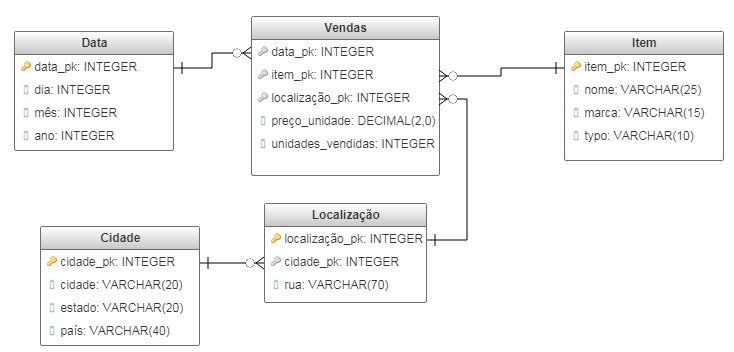
\includegraphics[width=13cm]{img/snow}
    \caption[Exemplo de esquema \textit{snowflake}]{Exemplo de esquema \textit{snowflake} \\ Adaptado da Figura \ref{fig:star_dim}}
	\label{fig:snow}
\end{figure*}

Para que possa ser construído um DW e aplicadas as modelagens acima descritas, 
é necessário alguma ferramenta que possa fazer o gerenciamento dele. 
De acordo com Elmasri e Navathe \cite{navathe2011banco} um banco de dados pode ser gerenciado por sistemas que 
facilitem este processo de gerenciamento no banco de dados. Antes de se ter um sistema que visava esse gerenciamento, entretanto, era utilizado para persistência de dados o sistema de arquivos. 

% SGBD ================================================================= %
\section{Sistemas Gerenciadores de Banco de Dados}

Apesar de simples, o sistema de arquivos apresentava alguns problemas por não oferecer suporte à redundância de informações; não garantir integridade de dados; 
falta de segurança; e o acesso e gerenciamento dos dados dependia de programas e aplicativos, fazendo com que seja necessário criar um novo aplicativo, ou adaptá-lo, a 
cada requisição de dados diferente. Outro problema crítico é não se ter informação de relacionamento entre arquivos diferentes.

Como forma de manter o gerenciamento de dados independente de aplicações e programas bem como solucionar os demais falhas do sistema de arquivos 
foram criados os Sistemas Gerenciadores de Banco de Dados, os SGBD. De acordo com Elmasri e Navathe \cite{navathe2011banco}, SGBD são uma coleção de programas para 
criação e manutenção de um banco de dados, que facilita a definição, construção, manipulação e compartilhamento de dados entre usuários e aplicações.

Dentre as vantagens que os SGBD trouxeram em detrimento ao sistema de arquivos estão:

\begin{itemize}
    \item{\textbf{Controle de redundância}}, para que não seja permitido duplicação de dados, pois isto causaria desperdício na capacidade de armazenamento.
    \item{\textbf{Restrição de acesso aos usuários}}, pois não será permitida manipulação do banco a todos os usuários, ou funcionários de uma empresa por exemplo.
    \item{\textbf{Execução de consultas eficiente}} através do uso de índices, normalmente implementadas utilizando hash ou árvores, para que o acesso ao disco seja mais rápido.
    \item{\textbf{Restrições de integridade}}, a fim de garantir que (i) dados não sejam inseridos de forma inconsistente de acordo com o tipo de atributo definido; 
    (ii) as relações entre entidades sejam efetuadas e (iii) restrições de chave sejam mantidas.
    \item{\textbf{Persistência de dados}}, para garantir que os dados serão inseridos e de fato armazenados no modelo.
    \item{\textbf{\textit{Backup}}} de dados periodicamente para evitar problemas caso aconteça alguma perda no banco e posterior \textbf{restauração}, para recuperar uma imagem do último backup feito no banco.
\end{itemize}

Existem várias classes de SGBD, conforme sua estruturação e a forma como manipulam os dados, 
entre as mais conhecidas estão o modelo relacional, objeto-relacional, orientado a 
objetos e a abordagem mais recente NoSQL.

\subsection{Modelo de SGBD Relacional}

O modelo mais utilizado de SGBD é o relacional, ou SGBDR (SGBD Relacional). Ele foi conceituado por 
Codd \cite{codd1970relational} em 1970 em um artigo no qual são expostas as 
vantagens de um modelo relacional em detrimento a um modelo de redes. 

Um modelo relacional define através de um conjunto de tabelas entidades que representam 
objetos do mundo real, cada qual com seus atributos. Esse conjunto de atributos é 
denominado registro do banco de dados, representando uma tupla, ou linha, na tabela. Assim como no mundo real, 
objetos devem estar também relacionados, e para tal SGBDR utilizam-se de chaves.

Em um SGBDR além de definir relacionamentos, as chaves também garantem integridade entre os dados. 
Existem dois tipos de chaves, uma que garante a unicidade de um atributo, ou seja, assegura que 
não haverão registros repetidos no banco tomando como referência aquele valor de chave, chamada de chave primária (do inglês \textit{Primary Key}, ou PK). A outra chave garante integridade no relacionamento entre duas entidades referenciando uma tabela na outra, que 
é a chave estrangeira (do inglês \textit{Foreign Key}, ou FK).

Tomando como exemplo uma empresa fictícia, são criados dois objetos reais que precisam ser 
representados sob a forma relacional, \textit{funcionário} e \textit{projeto}. Nesta empresa funcionários possuem \textit{nome, 
CPF, sexo, salário,} um \textit{supervisor} e trabalham em um ou mais \textit{projetos}. Esses projetos também possuem atributos: 
\textit{nome, código} e o número do \textit{departamento} no qual foram criados. Apenas com estas informações duas tabelas já são definidas 
no banco, \textit{funcionário} e \textit{projeto}, bem como seus atributos, como ilustra a Figura \ref{fig:func_proj}.

\begin{figure*}[htpb]
	\centering
		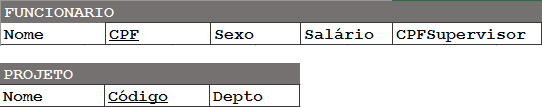
\includegraphics[width=13cm]{funcionario_projeto}
	\caption{Atributos das entidades \textit{funcionário} e \textit{projeto}}
	\label{fig:func_proj}
\end{figure*}

Como descrito, um funcionário trabalha em um ou mais projetos e ele precisa ainda registrar o número 
de horas trabalhadas nestes projetos. Desta forma é preciso de alguma forma relacionar funcionário com os projetos. 
Neste exemplo cabe a criação de uma nova entidade responsável unicamente por relacionar estes dois objetos e ainda 
armazenar o número de horas -- veja que o número de horas não cabe na tabela de funcionários nem na de projetos.

É nesta relação que são explorados os conceitos de chaves em um banco de dados. Para que a entidade que relaciona 
funcionário e projeto tenha informações de que funcionário trabalha em qual projeto é necessário acessar um número, ou código, 
definido para diferenciar todos os funcionários da empresa bem como o código do projeto e relacioná-los. Para o funcionário 
uma PK válida é o número do CPF e para o projeto o próprio atributo código. Essa relação pode ser nomeada unindo 
as entidades que relaciona, nesse caso \textit{funcionário\_projeto}, ou quando faz sentido pode ser nomeada de acordo com a função 
que realiza, neste caso como um funcionário trabalha em um projeto a relação pode ser \textit{trabalha\_em}.

O esquema que representa estas relações é como mostrado na Figura \ref{fig:relacao_func_proj}. Nela podemos ver as chaves primárias, em destaque, nas relações \textit{funcionário} e \textit{projeto}, e seus valores como chave estrangeira na relação \textit{trabalha\_em}. 

\begin{figure*}[htpb]
	\centering
		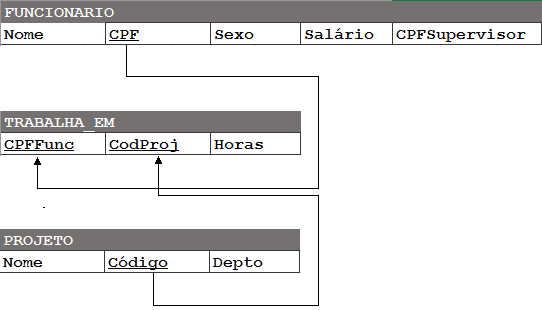
\includegraphics[width=13cm]{relacao_func_proj}
	\caption{Relacionamento entre \textit{funcionário} e \textit{projeto}}
	\label{fig:relacao_func_proj}
\end{figure*}

Modelos de bancos de dados prezam, sempre que possível, pela consistência de dados, principalmente se tomar operações transacionais como transações bancárias, que necessitam de um alto grau de consistência após operações de inserção e atualização, para que não haja perda de valores ou que esses ainda façam sentido no sistema. Por essa razão SGBDR seguem o conceito ACID (do inglês \textit{Atomicity, Consistency, Isolation, Durability}), o qual garante Atomicidade, Consistência, Isolamento e Durabilidade, ou Persistência, de dados. 

Modelos relacionais também seguem um alto grau de normalização nos dados a fim de evitar redundância e confusão entre atributos que podem ser desmembrados em outras entidades. Essa normalização é realizada normalmente até a Terceira Forma Normal, e o esquema final conterá um número maior de tabelas que o original devido ao desmembramento de atributos. Essa quantidade maior de tabelas acarreta no aumento de junções necessárias para recuperar atributos entre entidades relacionadas, ou seja, no aumento do acesso a entidades e no processamento de tuplas.

Além de diminuir o desempenho na recuperação de dados, um esquema normalizado causa um forte acoplamento entre tabelas, o que tornaria inviável o particionamento dos dados do banco em \textit{n} servidores como forma de escalar estes dados conforme seu volume aumenta, como é o caso de um ambiente analítico. Uma solução trivial para este problema é a denormalização de dados, porém para um SGBDR essa solução pode não ser viável, visto que sua implementação se dá seguindo a modelagem relacional.

Exemplos de SGBDR são PostgreSQL \cite{postgres2018r}, MySQL \cite{mysql2018r}, Microsoft SQL Server \cite{microsoft2018r}, SQLite \cite{lite2018r}, MariaDB \cite{maria2018r} e Oracle \cite{oracle2018r}. 

\subsection{Modelo de SGBD NoSQL}

% Bancos com o objetivo de suprir problemas apresentados por SGBDR começaram a emergir entre 2004 e 2007 visando alta escalabilidade, recuperação e armazenamento de grandes volumes de dados de forma eficiente, e ao mesmo tempo diminuir custos com hardware \cite{han2011nosql}. Esses bancos levaram o nome de NoSQL, porém isso não significa que não utilizam SQL para manipulação de dados.

% Detalhes sobre bancos de dados NoSQL são encontrados no Capítulo \ref{nosql}, no qual também é descrito o modelo colunar, utilizado por satisfazer os requerimentos de um ambiente de DW.

% \graphicspath{ {4-NoSQL/} }
% \chapter{Banco de Dados NoSQL}
% \label{nosql}

% NOSQL ==============================================================================================

O desenvolvimento de novas aplicações e surgimento de novas soluções 
para sistemas gerou crescimento no volume de dados de maneira acelerada. 
Com isso cresce também o número de usuários, necessitando portanto escalar 
o banco de dados. Existem duas soluções para escalar um sistema: o 
escalonamento vertical, que consiste em um \textit{upgrade} do servidor no 
qual o banco está hospedado; e o horizontal, aumentando o número de 
servidores e distribuindo o banco \cite{pritchett2008base, sharding2018educative}. 

Existem algumas desvantagens no \textit{upgrade} de um sistema. 
O banco de dados pode superar a capacidade da melhor configuração 
disponível no mercado, e ainda é caro por requerer a aquisição de 
uma configuração melhor. Mesmo considerado mais complexo, o 
escalonamento horizontal é mais viável. Entre as soluções apresentadas 
no particionamento horizontal em banco de dados estão o particionamento funcional e o 
\textit{sharding} \cite{pritchett2008base}. 

O particionamento funcional consiste em fragmentar os dados de acordo 
com a forma como são utilizados dado um contexto. Um esquema com quatro entidades, 
\textit{usuários}, \textit{produtos}, \textit{clientes} e \textit{endereço} 
pode ser distribuído em quatro servidores, 
um para cada entidade. Entidades que são utilizadas somente para leitura podem 
ser separadas de entidades onde dados são escritos, caracterizando outro 
exemplo de particionamento funcional. O problema com esta estratégia está 
no acoplamento entre entidades: se duas ou mais entidades estiverem 
relacionadas elas deverão estar no mesmo servidor, caso contrário não 
será possível atribuir as restrições de chave àquele relacionamento \cite{pritchett2008base}. 
Tomando o exemplo acima com as quatro entidades, supondo que \textit{cliente} 
e \textit{endereço} estejam relacionadas estas devem 
ser armazenados no mesmo servidor. 

A segunda estratégia, o \textit{sharding}, consiste em dividir os dados do banco 
utilizando algum critério de separação que não seja limitado à 
funcionalidade das entidades. Soluções como particionamento com base em 
\textit{hash} ou listas podem ser aplicadas. Considerando dez servidores e uma chave 
primária auto-incremental, a função de \textit{hash} pode tomar o módulo da chave 
primária pelo total de servidores como critério de seleção da partição 
na qual o dado será inserido. Utilizando uma lista é possível definir valores 
para os servidores e distribuir os dados de acordo com esses valores. 
Por exemplo, as linguagens C++, Java e C\# poderiam ser inseridas em uma 
partição destinada à linguagens orientadas a objeto.

O \textit{sharding} enfrenta problemas com junções entre dados, visto que os dados 
devem ser recuperados de diferentes partições e a maioria dos SGBDR não 
oferece suporte a chaves estrangeiras sob diferentes servidores, restando 
ao desenvolvedor tratar isso no código da aplicação \cite{pritchett2008base}. 
Uma solução para tais 
problemas é a denormalização de dados para que o número de junções diminua ou, 
no melhor dos casos e quando possível, seja zero. Contudo, isso é um problema 
para modelos relacionais, visto que trabalham sobre uma modelagem normalizada de dados. 
Além disso e de não se adaptarem à escalabilidade horizontal, 
são complexos e o fato de trazerem todas as informações de uma entidade sob a 
forma de tuplas causa lentidão em um ambiente analítico na recuperação de dados, 
cujas consultas percorrem o banco visando atributos específicos, processando 
somente o necessário. 

Outro problema crítico ao não utilizar a escalabilidade horizontal está na 
disponibilidade dos dados. Enquanto um banco se apoiar na escalabilidade vertical, 
qualquer queda no servidor acarretará na queda total no sistema de armazenamento, 
ao passo que quando se trabalha com servidores em paralelo a queda em uma máquina 
não trará prejuízos no conjunto todo. Assim, soluções como melhorar o hardware do 
servidor continuam sendo desvantajosas. 

Com o intuito de suprir tais problemas de escalabilidade, disponibilidade 
e recuperação rápida de dados, entre 2004 e 2007 os SGBD NoSQL começaram 
a ganhar destaque com o surgimento das bases de dados BigTable da Google \cite{chang2008bigtable}, e Dynamo 
da Amazon \cite{decandia2007dynamo}. O termo NoSQL, embora a princípio pareça indicar total independência 
de SQL, significa \textit{Not Only SQL}, “Não Apenas SQL”. Também, ele não descreve um 
único tipo de SGBD, mas sim uma classe de modelos, cada qual com suas propriedades. 
As mais conhecidas são quatro:

\begin{itemize}
    \item{\textbf{Orientado a Grafos}}, que se utiliza da Teoria dos Grafos para estruturar seus dados. 
    Um exemplo desta classe é o Neo4j \cite{neo2018nosql}.
    \item{\textbf{Orientado a Chave-Valor}}, que armazena os dados de forma similar a uma tabela \textit{hash}, 
    com uma chave referenciando um valor, ou tipo de dado. Exemplos são o Project Voldemort \cite{voldemort2018nosql}, 
    DyanmoDB \cite{amazon2018nosql}, o Riak \cite{riak2018nosql} e o Redis \cite{redis2018nosql}.
    \item{\textbf{Orientado a Documento}}, uma versão melhorada do Chave-Valor, 
    no qual os valores são armazenados como documentos através de estruturas complexas como JSON e XML. 
    Exemplos são o MongoDB \cite{mongo2018nosql} e o CouchDB \cite{couch2018nosql}.
    \item{\textbf{Orientado a Colunas}}, ou modelo colunar, 
    que utiliza tabelas como armazenamento de entidades, 
    porém não agrupa os dados sob forma de tuplas, e sim colunas. Exemplos são o MonetDB \cite{monetdb2017c}, C-Store \cite{cstore2018nosql}, BigTable \cite{google2018nosql} e Cassandra \cite{cassandra2018nosql}.
\end{itemize}

De maneira geral, as vantagens no uso de um SGBD NoSQL estão no rápido processamento de um grande volume de dados, flexibilidade para expansão e baixo custo de escalabilidade. Devido ao vasto número de SGBD dentro de cada classe de NoSQL, esses banco de dados também podem ser classificados de acordo com o Teorema CAP (do inglês \textit{Consistency, Availability, Partition tolerance}). Segundo Eric Brewer \cite{brewer2000towards, gilbert2002brewer}, um sistema distribuído não é 
capaz de conciliar consistência, disponibilidade e tolerância a partição de dados simultaneamente, tendo que optar por apenas dois destes. 
SGBDR prezam por disponibilidade e consistência de dados seguindo ACID, porém, a preocupação com consistência 
pode tornar a manipulação de dados lenta. Visto que o movimento NoSQL surgiu com a intenção de 
melhorar a escalabilidade e disponibilidade de dados, e tornar a manipulação destes mais rápida, 
a maioria deles trabalha com os atributos de disponibilidade e tolerância à partição. 
Essa configuração assume um conceito diferente do ACID para bancos NoSQL, e Pritchett \cite{pritchett2008base} propôs um teorema diferente deste, mais otimista, onde a consistência é relaxada, o Teorema BASE (\textit{Basically Available, Soft State, Eventual Consistency}).

O Teorema BASE assume que a consistência em um banco 
de dados está em estado de fluxo, ao contrário de ACID que força a consistência a cada operação, 
sendo este considerado por Pritchett \cite{pritchett2008base} um método pessimista. 
Neste cenário a disponibilidade é garantida devido à tolerância a partição, fazendo 
com que a falha de um servidor não cesse o funcionamento de todo o sistema -- por exemplo, caso uma partição falhe em um sistema rodando sobre dez servidores, apenas 10\% dos dados estarão indisponíveis e somente os usuários daquela partição serão afetados.

% COLUNAR =============================================================================

% \subsubsection{Modelo de SGBD NoSQL Colunar}

Dentre as categorias de bancos de dados NoSQL citadas a que melhor se adequa aos 
propósitos analíticos é a colunar. Sistemas colunares armazenam seus dados 
em colunas que representam atributos das entidades, fazendo com que apenas os atributos necessários sejam 
lidos \cite{khoshafian1987query}, o que diminui o tempo de acesso 
ao disco \cite{matei2010column, abadi2008column}. Cada uma destas colunas pode armazenar seus valores utilizando o par 
\textit{chave, valor} \cite{abadi2013design, khoshafian1987query}, sendo esta uma das formas de implementação 
de um sistema colunar. 
A Figura \ref{fig:row-col} ilustra de forma simples, embora apenas visual, 
a diferença principal entre um armazenamento utilizando linhas, conforme a Figura \ref{fig:row}, e outro utilizando 
colunas, Figura \ref{fig:column}, a partir dos registros da Figura \ref{fig:regs}, baseada na entidade \textit{funcionário} apresentada no Capítulo \ref{sgbd}.

% (descrita na Seção \ref{sec:implementacao_col} deste capítulo)

\begin{figure*}[htpb]
	\centering
		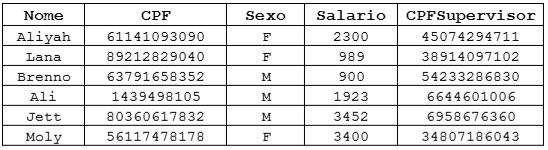
\includegraphics[width=12cm]{registros}
	\caption{Exemplos de registros para a entidade \textit{funcionário} apresentada na seção anterior}
	\label{fig:regs}
\end{figure*}

\begin{figure*}[htpb]
    \centering
    \subfigure[]{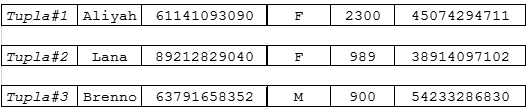
\includegraphics[width=8cm]{row}\label{fig:row}}
    \subfigure[]{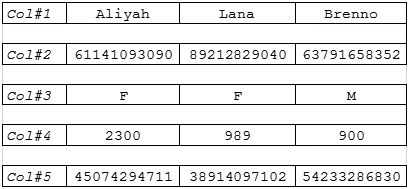
\includegraphics[width=6.8cm]{column}\label{fig:column}}
    \caption{Diferença visual entre registros armazenados em um banco relacional e colunar}
    \label{fig:row-col}
\end{figure*}

Matei \cite{matei2010column} cita algumas vantagens de sistemas colunares:

\begin{itemize}

    \item{\textbf{Melhor desempenho}}, pela forma com que os dados são armazenados e o uso de índices 
    visando o armazenamento ao invés de localização de registros, resultando em menos operações de 
    entrada e saída.
    \item{\textbf{Rápidas operações de agrupamento}}, bastante utilizadas em ambientes OLAP, visto 
    que valores de um mesmo atributo são armazenados consecutivamente. Bem como operações matemáticas, 
    como recuperar o maior ou menor valor, soma e média.
    \item{\textbf{Alta compressão de dados}} pode ser alcançada, devido às chances de se ter 
    valores repetidos para um mesmo atributo serem maiores.

\end{itemize}

Existem diferentes abordagens para se implementar um SGBD colunar. Essas abordagens levam em conta 
mudanças na codificação de um banco, apenas na modelagem dele, bem como se será possível atingir 
níveis altos de compressão. A primeira técnica consiste no \textbf{particionamento vertical} dos dados, a 
segunda em \textbf{modificar a camada de armazenamento} e a terceira corresponde a junção de ambas.

% \subsection{Implementação do Sistema Colunar}
% \label{sec:implementacao_col}

Antes de detalhar os métodos de implementação de um banco de dados colunar, é fundamental discutir sobre a reconstrução de tuplas nesse tipo de SGBD. 
Segundo Abadi et al. \cite{abadi2007materialization}, a parte lógica e visual de um banco de dados colunar se apresenta da mesma forma que 
um relacional. Isso faz com que a maioria dos SGBD colunares ofereçam uma interface relacional de comunicação, compatível com os padrões.

Como os atributos de um modelo colunar acabam ficando separados em disco um do outro, eles precisam ser unidos novamente em tuplas para 
que o resultado de uma consulta seja exibido. Existem duas técnicas para realizar essa reconstrução, ou materialização: \textit{Early Materialization} (EM) e 
\textit{Late Materialization} (LM) \cite{abadi2007materialization, abadi2008query}.

A técnica de \textit{Early Materialization}, melhor traduzida como materialização prévia nesse contexto, é a política adotada por banco de dados relacionais, e consiste 
em adicionar as colunas à tupla conforme a coluna é requisitada na consulta. Essa técnica não leva em conta o predicado da consulta. Como exemplo, considere a consulta a seguir:

\begin{lstlisting}[language=SQL,label=sql_1]
                    SELECT nome FROM funcionario 
                    WHERE salario >= 1000 AND sexo='F'
\end{lstlisting}

A EM irá processar essa consulta e construir uma tupla com os atributos \textit{nome, salário} e \textit{sexo}, com todos os registros 
armazenados em banco. Considere que os registros são como mostrados na Figura \ref{fig:regs}, o construtor de tuplas retornará os registros conforme a Figura \ref{fig:em}. Esse método só analisa o predicado após a construção das tuplas, o que não acontece na LM. 

\begin{figure*}[htpb]
	\centering
        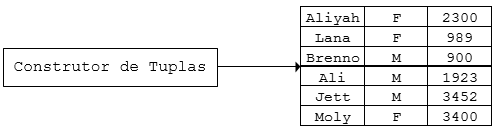
\includegraphics[width=14cm]{em}
	\caption{Tuplas reconstruídas a partir da \textit{Early Materialization}}
	\label{fig:em}
\end{figure*}

Na LM, ou materialização tardia, é analisado primeiro o predicado e verificado quais valores atendem a esse predicado em cada coluna. 
No caso da SQL acima primeiro seria analisado o predicado de seleção, nesse caso \texttt{WHERE salario >= 1000 AND sexo='F'}, e então 
através do operador lógico AND seria possível retornar a posição dos atributos que satisfazem essa seleção, para então 
construir a tupla a partir do predicado de projeção somente com o atributo \textit{nome}. Em suma, apenas após ter a posição de cada atributo é que a tupla é construída, descartando a reconstrução de tuplas que seriam posteriormente descartadas. A Figura \ref{fig:lm} apresenta o resultado após a construção das tuplas na LM.

\begin{figure*}[htpb]
	\centering
        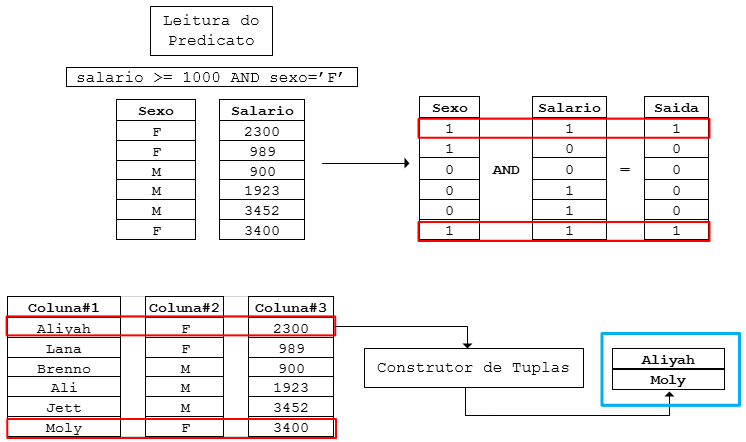
\includegraphics[width=14cm]{lm}
	\caption{Tuplas reconstruídas a partir da \textit{Late Materialization}}
	\label{fig:lm}
\end{figure*}

% inserir subfigure com tuplas

% \subsection{Particionamento Vertical}

A primeira técnica de implementação de um banco de dados colunar consiste no particionamento vertical dos dados. Considerada a técnica mais simples para implementar um banco colunar, esta técnica 
realiza a partição dos dados de forma que cada atributo de uma entidade seja armazenado 
em uma tabela de duas colunas contendo o par <chave/índice, valor do atributo> \cite{khoshafian1987query}.

% inserir figura de particionamento vertical

A Figura \ref{fig:vertical} mostra que é possível desmembrar o esquema relacional da Figura \ref{fig:regs} em colunas de atributos -- foram desmembrados os atributos \textit{nome, sexo} e \textit{salario}. 
No momento em que uma consulta analítica é realizada, não serão processados dados além 
dos de fato requeridos e nenhum dado é perdido pois ainda haverá referência entre os atributos 
através das chaves.

\begin{figure*}[htpb]
	\centering
        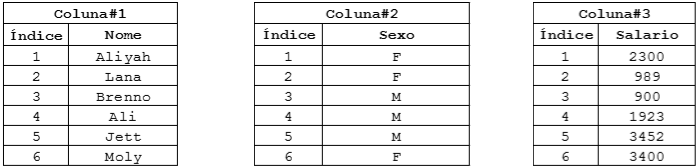
\includegraphics[width=\textwidth]{vertical}
	\caption{Implementação do modelo colunar utilizando particionamento vertical}
	\label{fig:vertical}
\end{figure*}

Essa abordagem é a mais simples de se implementar, pois nenhuma mudança é feita 
na codificação do banco de dados, sendo que a única alteração necessária está a nível 
da aplicação responsável por executar as consultas, mudando a lógica de acesso aos dados. Isso torna prático para empresas a 
mudança entre a estratégia relacional e a colunar, pois torna possível o uso de um mesmo 
SGBD como DW.

Ao mesmo tempo que essa implementação traz praticidade na migração de dados, ela não difere 
muito da abordagem relacional no que concerne ao desempenho. Em Abadi \cite{abadi2008query} 
é mostrado que adaptar dados de um esquema relacional utilizando particionamento vertical não 
trouxe melhoras no desempenho das consultas. Foi verificado que o custo de junções para unir 
as colunas é alto conforme a quantidade de atributos selecionados aumenta e não foi possível 
usufruir eficientemente da compressão de dados.

% \subsection{Modificação na Camada de Armazenamento}

A segunda abordagem para implementar um sistema colunar consiste em já modificar o armazenamento do banco. Essa técnica não altera a parte 
lógica da modelagem do banco, mas a camada física alterando o armazenamento de 
linha por linha para coluna por coluna. Nessa implementação as chaves não precisam ser 
repetidas como na abordagem anterior, na qual a primeira coluna de cada tabela 
consistia no valor de chave da cada atributo. O \textit{i-ésimo} valor de atributo 
de uma coluna estará associado ao \textit{i-ésimo} atributo das demais colunas e 
não é desperdiçado espaço em disco com as chaves.

Neste método a reconstrução de tuplas é realizada antes da execução da consulta de fato. Como apenas um determinado número de atributos precisa ser acessado, estes são combinados seguindo a lógica que o \textit{i-ésimo} atributo de uma coluna está relacionado com o \textit{i-ésimo} atributo das demais. Aqui tem-se uma vantagem no modelo orientado a linhas, por este já armazenar as sob o formato de linhas e não precisar armazenar os dados em ordem.

% \subsection{Modificação na Camada de Armazenamento e Particionamento Vertical}

A última, e melhor, abordagem consiste em modificar a camada de armazenamento do banco de dados e a aplicação que processa as consultas \cite{stonebraker2005c, boncz2005monetdb}, assim o processador pode manter os dados sob a forma de colunas sem precisar unir as colunas e construir tuplas. Uma vantagem óbvia desta técnica é a eliminação da reconstrução de tuplas e com isso menos dados precisam ser previamente movimentados, diminuindo 
o tempo de processamento.  

% \section{Compressão de Dados}

Além da diferença na implementação, e por consequência disso, uma característica marcante de um SGBDC é a alta possibilidade de compressão de dados. 
Existem diversas formas de comprimir os dados, porém deve-se ater ao fato de 
que o tempo de compressão e descompressão não deve afetar significativamente o processamento 
dos dados no SGBD. Para tal, uma solução é utilizar métodos que consigam operar sob os dados 
ainda comprimidos -- ainda nesta seção são apresentados alguns dos algoritmos utilizados para 
compressão em banco de dados.

Como exemplo, apenas ilustrativo, de como os dados em um sistema colunar podem ser comprimidos de forma mais 
eficiente que em um relacional, considere a entidade \textit{usuário} a seguir, com os 
atributos \textit{id, nome, idade} e \textit{sexo}. A primeira coluna corresponde aos índices utilizados no banco. 

\begin{verbatim}
    1: 0, Bruno, 50, M
    2: 10, João, 23, M
    3: 20, Maria, 30, F
    4: 90, Ana, 23, F
    5: 78, Gabriel, 23, M
\end{verbatim}

Um banco relacional armazena estes atributos da forma como foram apresentados acima. 
Considerando o armazenamento colunar, os mesmos dados seriam armazenados da seguinte forma: 

\begin{verbatim}
    1: 0, 2: 10, 3: 20, 4: 90, 5: 78
    1: Bruno, 2: João, 3: Maria, 4: Ana, 5: Gabriel
    1: 50, 2: 23, 3: 30, 4: 23, 5: 23
    1: M, 2: M, 3: F, 4: F, 5: M
\end{verbatim}

Note que fica mais claro que como os atributos são armazenados em uma coluna com chave e valor 
existirão mais chances de repetição de valores em uma mesma coluna. Os atributos \textit{idade} e 
\textit{sexo} se repetem para alguns registros, possibilitando assim compressão destes dados. 
Comprimindo estas repetições o nosso modelo é armazenado da forma: 

\begin{verbatim}
    1: 0, 2: 10, 3: 20, 4: 90, 5: 78
    1: Bruno, 2: João, 3: Maria, 4: Ana, 5: Gabriel
    1: 50, 2, 4, 5: 23, 3: 30
    1, 2, 5: M, 3, 4: F
\end{verbatim}

Westmann \textit{et al.} \cite{westmann2000implementation} consideram que os métodos de compressão em um banco de dados devem ser capazes de se aplicar 
no banco como um todo, bem como em uma tupla ou a cada atributo de tupla, e serem rápidos em processamento quando há casos em que seja 
necessário realizar descompressão.

O primeiro método consiste em comprimir a representação de valores inteiros, baseado no algoritmo \textit{null supression} \cite{westmann2000implementation, roth1993database}. A ideia é descartar zeros na representação de um inteiro de quatro bytes, por exemplo, 
ao invés de se representar o número 10 da forma '00000000000000000000000000001010', seriam utilizados apenas quatro bits, '1010'. É 
necessário entretanto, guardar a informação de quantos bits são utilizados para armazenar um número e em alguns casos também é preciso 
armazenar um bit a mais para o sinal do inteiro. Esse algoritmo pode ser utilizado para comprimir o tamanho de strings no banco 
quando estas são representadas pelo tipo VARCHAR, visto que para esse tipo de dado o tamanho também é armazenado devido a possibilidade 
deste variar.

Um método bastante empregado é a Codificação por Dicionário. Nele atributos que possuem um padrão fixo, por exemplo, os números primos de 
3 a 19 (3, 5, 7, 11, 13, 17, 19), podem ser representados por um dicionário de 3 bits. Este algoritmo pode ser utilizado para compressão 
de valores NULL, considerando-o como um possível valor no padrão.

Abadi, Madden e Ferreira \cite{abadi2006integrating} utilizam a compressão por dicionário e uma variação do algoritmo \textit{null supression} para implementar o banco de dados C-Store e ainda apresentam dois outros métodos. O primeiro é o \textit{run-length}, que pode ser bem aproveitado 
em bancos colunares quando atributos são repetidos sequencialmente e possuem pouca variação. Ele consiste em contar o número de vezes no qual 
um valor é repetido utilizando a tripla (valor, posição inicial, tamanho). 
% Um exemplo é ilustrado na Figura A com o atributo \textit{especialização}.



% inserir uma imagem run length com graduação, mestrado, doutorado.

O último método apresentado pelos autores é a Codificação por Vetor de Bit, bastante útil quando uma coluna possui número limitado 
de possibilidades, como linguagens de programação dentro de um dado paradigma ou estados do Brasil. Uma string de bits representa a 
ocorrência do valor de atributo, onde '1' representa a ocorrência naquela posição e '0' a não ocorrência. Como exemplo, uma coluna com os 
valores {M M F M F F M} podem ser representados pela cadeia de bits 1 1 0 1 0 0 1 para o valor M, e 0 0 1 0 1 1 0 para F.

Em suma, ao implementar um banco colunar tanto a aplicação deve ser capaz de entender e conseguir recuperar informações mesmo comprimidas, como a modificação da camada de armazenamento deve ser implementada tal que se possa usufruir de algum método de compressão. Caso contrário um 
dos principais diferenciais de modelos colunares não será explorado e poderá não haver impacto no desempenho quando trabalhado com uma 
grande massa de dados, como é a realidade de empresas.

\section{Considerações Finais}

% data warehouses e olap -> modelo denormalizado -> sgbdr x sgbdc

Tendo surgido como solução para dar suporte à tomada de decisão, DWs precisam ter seus dados recuperados de forma eficiente. A principal discussão acerca disso está em torno de qual modelagem utilizar e como realizar o gerenciamento deste repositório de forma a conseguir um bom desempenho na recuperação de dados como informação útil à uma empresa. Como solução a isso estão os SGBDR, entretanto, seu uso causa queda no desempenho conforme o volume de dados aumenta, para tanto são necessários outros meios de gerenciamento que possam lidar com esse grande volume de dados.

Apresentando soluções aos impasses de um SGBDR estão os SGBD NoSQL, e dentre suas classes a que melhor supre as necessidades de um ambiente analítico é a colunar. Com uma implementação diferente da utilizada pelos SGBDR, este SGBD possibilita altas taxas de compressão e recuperação de atributos específicos sem processar mais do que o requisitado por uma consulta. 

Empresas ainda utilizam SGBDR para gerenciar DWs, e para analisar qual SGBD é melhor nesta função pode-se aplicar alguma métrica para cálculo de desempenho e comparar um com o outro, ou vários. Esse cálculo deve considerar ainda as possíveis modelagens entre os SGBD, possibilitando adaptar diferentes modelagens dentro de um DW. Na área de banco de dados são utilizados \textit{benchmarks} produzidos por empresas com foco em desenvolver padrões no processo de transações.
\chapter{TPC \textit{Benchmark} H}
\label{tpch}

A essência de um \textit{benchmark} é identificar e definir os melhores padrões de excelência para produtos, serviços e/ou processos, e então realizar aperfeiçoamentos de forma que esses padrões sejam alcançados \cite{bhutta1999benchmarking}. De maneira geral, \textit{benchmarks} se consolidaram como uma ferramenta para melhorar o desempenho de organizações e a competitividade nos negócios \cite{kyro2003revising}.

O TPC \textit{\textit{benchmark}} H é um padrão de decisão de negócio internacionalmente aceito para comparações de desempenho entre SGBDs utilizados em ambientes OLAP criado pela organização TPC. De acordo com a página oficial do TPC\footnote{http://www.tpc.org/information/about/abouttpc.asp}, esta organização sem fins lucrativos foi fundada com o objetivo de definir padrões para \textit{benchmarks} no processamento de transações e bancos de dados. Ela é responsável pelo desenvolvimento e atualização destes \textit{benchmarks}, bem como pela divulgação dos resultados apresentados por eles. Entre os sócios\footnote{Lista de sócios acessada em Junho de 2017} responsáveis por isto estão as empresas Dell, Hewlet Packard, IBM, Microsoft, Oracle, Intel e Cisco. A lista de todos os sócios pode ser acessada na página oficial da organização.

Alguns trabalhos já foram realizados utilizando o TPC-H \cite{ngamsuriyaroj2010performance, nadee2012performance, thanopoulou2012benchmarking, barata2014ycsb, rutishauser2012tpc, soares2012avaliaccao}. Ngamsuriyaroj e Pornpattana \cite{ngamsuriyaroj2010performance} aplicam as consultas do TPC-H no MySQL Cluster a fim de avaliar seu desempenho. O trabalho de Nadee e Ngamsuriyaroj \cite{nadee2012performance} tem uma proposta parecida com o primeiro \cite{ngamsuriyaroj2010performance}, porém o intuito é avaliar o desempenho de um \textit{cluster} Java EE baseado nas características das consultas do TPC-H. Thanopoulou et al. \cite{thanopoulou2012benchmarking} foca em aplicar o TPC-H em bancos de dados de pequenas empresas que não podem arcar com configurações de \textit{hardware} melhores para administrar um banco de dados. Barata, Bernardino e Furtado \cite{barata2014ycsb} fazem uma descrição teórica de dois \textit{benchmarks}, o YCSB (\textit{Yahoo Cloud Serving Benchmark}), voltado para a área de \textit{Big Data}, e o TPC-H. Rutishauser e Noureldin \cite{rutishauser2012tpc} realizam uma análise comparativa entre PostgreSQL e MongoDB aplicando o TPC-H. O primeiro é um SGBD relacional clássico, e o outro um SGBD NoSQL com algumas consultas do TPC-H adaptadas. Por fim, Soares \cite{soares2012avaliaccao} compara SGBD relacionais e colunares executando um teste de força sob o \textit{Star Schema Benchmark} simulando bases de dados de 1Gb, 2Gb, 5Gb e 10Gb.

De acordo com o manual de especificação fornecido pelo TPC \cite{tpc2017specs}, o TPC-H é um \textit{\textit{benchmark}} de suporte à decisão de negócios, constituído de uma série de consultas comerciais \textit{ad-hoc} e modificações simultâneas de dados com finalidade de retratar a realidade das empresas. Ele representa DSS que examinam grandes volumes de dados; executam consultas com um alto grau de complexidade; e respondem questões críticas de negócio. Como o \textit{\textit{benchmark}} trata de grandes volumes de dados, o tamanho mínimo de banco de dados proposto pelo TPC-H é de 1GB, seguido por 10GB, 30GB, 100GB, 300GB, 1000GB, 3000GB, 10000GB, 30000GB e 100000GB. Estes valores também correspondem ao Fator de Escala (\textit{Factor Scale} -- SF). 

Com o intuito de avaliar o resultado do desempenho de SGBDs como DW, é necessário ter conhecimento de como os dados que irão popular o DW estão distribuídos. Para tal, o TPC-H propõe um ambiente normalizado \textit{Snow Flake}. Ele é composto por oito tabelas e é descrito na Seção \ref{ambiente_1}. Do mesmo modo, a fim de obedecer as regras de modelagem deste ambiente, é preciso ter dados conhecidos para popular os DWs. Estes dados são fornecidos pelo \textit{software} DBGen.

O DBGen foi implementado pelo TPC-H, com o objetivo de realizar a população de dados em um DW seguindo a modelagem original \textit{Snow Flake}. São gerados oito arquivos separados no formato \texttt{<nome da tabela>.tbl} -- exemplificando, a tabela de dados \textit{Part} será gerada como \texttt{part.tbl}; onde as linhas de cada arquivo representam as tuplas dentro da respectiva tabela, tendo seus atributos separados por um delimitador \textit{pipe} ("$\mid$"). Por padrão, os arquivos são gerados para uma base de dados da classe de 1GB, quando nenhum SF é especificado.

Assim como é necessário conhecer os dados de modo a seguir a modelagem proposta pelo \textit{benchmark}, é preciso formular consultas que visam responder às questões de negócio definidas pelo TPC-H sobre o modelo de dados. O próprio TPC define para seu modelo 22 consultas, cada qual definida por (i) uma questão de negócio, que ilustra o contexto no qual a consulta pode ser aplicada; (ii) uma definição funcional, que corresponde à implementação da consulta utilizando a Linguagem SQL-92; (iii) parâmetros de substituição, que geram os valores necessários para completar os parâmetros da consulta; e (iv) validação, que descreve como validar a consulta no BD. Igualmente à geração de dados, a geração de consultas também é feita com o uso de um programa fornecido pelo TPC, o QGen.

Com o QGen é possível gerar as consultas de acordo com a especificação do TPC-H inserindo os parâmetros de substituição adequados em cada uma. A Consulta 1 presente no Apêndice \ref{queries_1}, Consulta de Relatório de Resumo de Preços, possui o parâmetro de substituição [DELTA], correspondente a um número inteiro entre 60 e 120, inserido ao executar o programa QGen para a respectiva consulta. Esses valores podem ser inseridos de maneira aleatória, entretanto o TPC-H define valores padrão para os parâmetros de substituição para fins de validação; portanto as consultas no QGen são geradas utilizando os valores padrão. As 22 consultas com suas respectivas questões de negócio e parâmetros de substituição são descritas no Apêndice \ref{queries_1}.

\section{Metodologia}
\label{metodologia}

Após a geração dos arquivos é criado em cada SGBD um esquema correspondente às classes utilizadas, tanto para o Ambiente Normalizado quanto para o Desnormalizado. Cada SGBD é então executado sobre os dois ambientes propostos. Em cada ambiente será executado o teste de performance, que consiste de duas execuções: o Teste de Força (\textit{Power Test}) e o Teste de Vazão (\textit{Throughput Test}), descritos nas Subseções \ref{power_test} e \ref{through_test}, respectivamente. O tempo resultante de cada etapa é utilizado para calcular o desempenho final do SGBD, medido em \textit{QphH@Size} -- quantidade de consultas executadas por hora, dada uma classe de tamanho de banco de dados. Uma execução é composta por:

\begin{itemize}
	\item \textit{SF}, que representa a classe do banco de dados.
	\item \textit{$Q_{i}$}, que representa uma consulta, onde \mbox{$1 \le i \le 22$}.
	\item \textit{S}, que define o número de sessões de consulta do Teste de Vazão.
	\item \textit{s}, que representa uma dada sessão, onde \mbox{$1 \le s \le S$}.
	\item \textit{$T_{s}$}, que representa o tempo, em segundos, resultante do processo inteiro.
	\item \textit{$RF_{j}$}, que representa a Função de Atualização (\textit{Refresh Function} -- RF), onde:
		\begin{itemize}
		    \item RF1: inserção de novos registros. O número de registros inseridos deve ser igual para o número de registros removidos pela RF2. O pseudocódigo para a RF1 é como:
		
\begin{verbatim}
    loop (SF * 1500) times
        insert <new row into> ORDERS table
        loop random(1, 7) times
            insert <new row into> LINEITEM table
        end loop
    end loop
\end{verbatim}
		    \item RF2: remoção de registros antigos. O pseudocódigo para a RF1 é como:
		
\begin{verbatim}
    loop (SF * 1500) times
        delete from ORDERS where O_ORDERKEY = [valor]
        delete from LINEITEM where I_ORDERKEY = [valor]
    end loop
\end{verbatim}
		\end{itemize}
\end{itemize}

O conjunto de dados para executar com sucesso as RFs também são gerados pelo DBGen utilizando a \textit{flag} -U.

\subsection{Teste de Força}
\label{power_test}
O Teste de Força objetiva medir a execução de uma dada consulta do sistema com um único usuário ativo. Neste teste é criada uma única sessão com o respectivo SGBD e as seguintes instruções são executadas:

\begin{itemize}
	\item Execução da RF1.
	\item Execução de cada consulta proposta pelo TPC-H, ou adaptada, de forma sequencial uma única vez até a última consulta.
	\item Execução da RF2.
\end{itemize}

Será armazenado ao fim do teste o tempo em segundos resultante de cada consulta, bem como o tempo de execução de cada função. Este resultado será utilizado na Equação \ref{eq:1}.

\begin{myequation}%
\label{eq:1}
{\scriptstyle Power@Size} = \frac{3600 * SF}{\sqrt[24]{\prod_{i = 2}^{i = 22}Q(i, 0) * \prod_{j = 1}^{j = 2}RF(j, 0)}} %
\end{myequation}
%

\subsection{Teste de Vazão}
\label{through_test}
Este teste mede a capacidade do sistema de processar a maior quantidade possível de consultas no menor intervalo de tempo. Aqui o TPC-H exige um número mínimo de sessões de consulta de acordo com a classe de tamanho do banco de dados, como mostra a Tabela \ref{min_sessions}.

\begin{table}[htpb]
\centering
\caption{Número mínimo de sessões para uma classe de banco de dados}
\label{min_sessions}
\begin{tabular}{|c|c|}
\hline
\multicolumn{1}{|c|}{\textbf{Classe do Banco de Dados}} & \textbf{Número de Sessões} \\ \hline
1 GB                                      & 2                            \\ \hline
10 GB                                      & 3                          \\ \hline
30 GB                                        & 4                             \\ \hline
100 GB                                        & 5                             \\ \hline
300 GB                                        & 6                             \\ \hline
1000 GB                                        & 7                             \\ \hline
3000 GB                                        & 8                             \\ \hline
10000 GB                                        & 9                             \\ \hline
30000 GB                                        & 10                             \\ \hline
100000 GB                                        & 11                             \\ \hline
\end{tabular}
\end{table}

É criada uma sessão para executar as Funções e \textit{N} sessões para executar as consultas, de acordo com a Tabela \ref{min_sessions}. As instruções são executadas concorrentemente. Para a sessão das Funções, as seguintes instruções são executadas:

\begin{itemize}
	\item A RF1 e RF2 deverão ser executadas sequencialmente \textit{N} vezes, onde \textit{N} é o número de sessões para a execução de consultas.
	\item Para cada sessão de consultas, cada consulta será executada sequencialmente até a última.
\end{itemize}

Ao fim do teste, é armazenado o tempo em segundos da execução do processo inteiro. O processo inicia quando a primeira sessão, seja de consulta ou de Função, executa sua instrução e finaliza quando a última sessão recebe uma resposta. O resultado é utilizado para calcular o desempenho do SGBD para o Teste de Vazão conforme a Equação \ref{eq:2}.

\begin{myequation}%
\label{eq:2}
{\scriptstyle Throughput@Size} = \frac{S * 22 * 3600}{T_s * SF} %
\end{myequation}
%

O resultado dos cálculos de Força e Vazão serão utilizados para calcular o desempenho final do SGBD da seguinte forma:

\begin{myequation}%
\label{eq:3}
{ \scriptstyle QphH@Size = \sqrt{Power@Size * Throughput@Size} } %
\end{myequation}
%

\section{Ambiente Original Normalizado}
\label{ambiente_1}

O modelo de ambiente proposto pelo TPC-H é um esquema normalizado \textit{Snow Flake}. Ele é composto por oito tabelas, sendo que destas, seis têm o tamanho multiplicado por um Fator de Escala, que corresponde ao tamanho da classe do banco de dados; enquanto que as demais, \textit{NATION} e \textit{REGION}, têm tamanho fixo. O relacionamento \textit{one-to-many} entre as tabelas do esquema \textit{Snow Flake} é apresentado na Figura \ref{fig:snow_flake}, adaptada do manual de especificação do TPC-H \cite{tpc2017specs}.

\begin{figure*}[h]
	\centering
		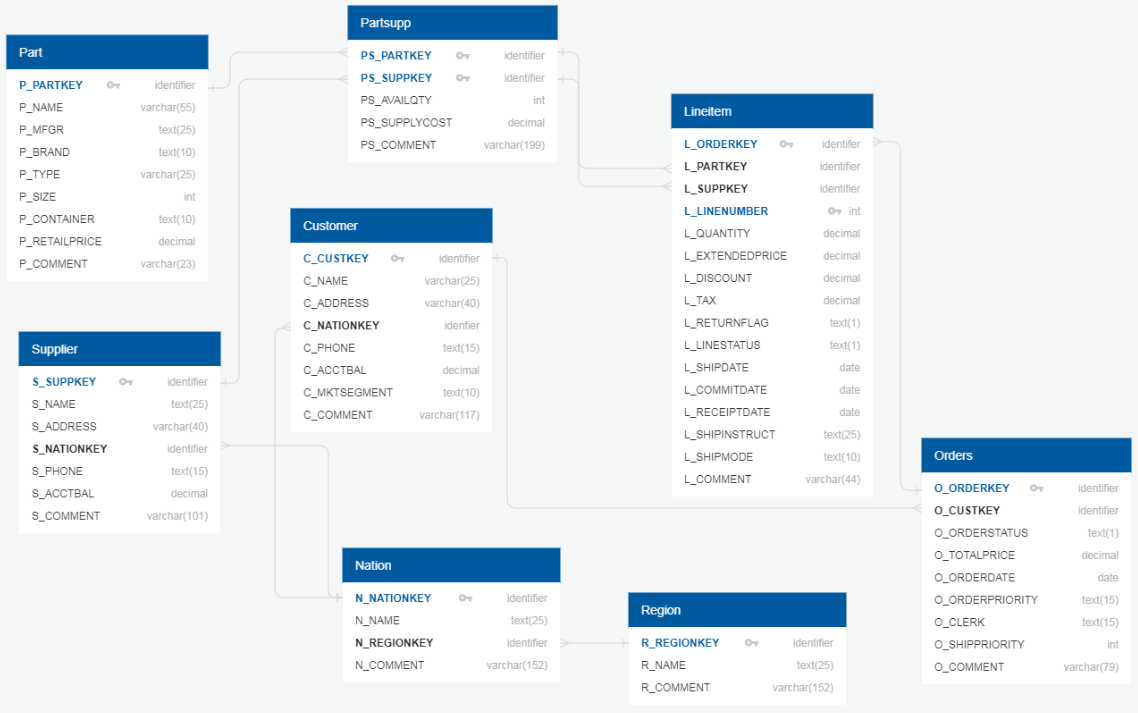
\includegraphics[width=\textwidth]{img/snow_flake.png}
	\caption{Esquema do ambiente normalizado}
	\label{fig:snow_flake}
\end{figure*}

\begin{comment}
\begin{table}[h]
\centering
\caption{Dados para a classe de 1GB}
\label{1gb_table}
\begin{tabular}{|l|c|c|}
\hline
\multicolumn{1}{|c|}{\textbf{Nome da tabela}} & \textbf{Cardinalidade} & \textbf{Tamanho} \\ \hline
CUSTOMER                                      & 150 K                  & 23.3 MB          \\ \hline
LINEITEM                                      & 6 M                    & 730 MB           \\ \hline
NATION                                        & 25                     & 2.19 KB          \\ \hline
ORDERS                                        & 1.5 M                  & 165 MB           \\ \hline
PART                                          & 200 K                  & 23.2 MB          \\ \hline
PARTSUPP                                      & 800 K                  & 114 MB           \\ \hline
REGION                                        & 5                      & 394 Bytes        \\ \hline
SUPPLIER                                      & 10 K                   & 1.35 MB          \\ \hline
Total																					&												 & 								\\ \hline
\end{tabular}
\end{table}

\begin{table}[h]
\centering
\caption{Dados para a classe de 10GB}
\label{10gb_table}
\begin{tabular}{|l|c|c|}
\hline
\multicolumn{1}{|c|}{\textbf{Nome da tabela}} & \textbf{Cardinalidade} & \textbf{Tamanho} \\ \hline
CUSTOMER                                      & 1.5 M                  & 234 MB          	\\ \hline
LINEITEM                                      & 60 M                   & 7.29 GB          \\ \hline
NATION                                        & 25                     & 2.19 KB          \\ \hline
ORDERS                                        & 15 M                   & 1.64 GB          \\ \hline
PART                                          & 2 M                  	 & 233 MB          	\\ \hline
PARTSUPP                                      & 8 M                  	 & 1.12 GB          \\ \hline
REGION                                        & 5                      & 394 Bytes        \\ \hline
SUPPLIER                                      & 100 K                  & 13.6 MB          \\ \hline
Total																					&												 & 								\\ \hline
\end{tabular}
\end{table}

\begin{table}[h]
\centering
\caption{Dados para a classe de 30GB}
\label{30gb_table}
\begin{tabular}{|l|c|c|}
\hline
\multicolumn{1}{|c|}{\textbf{Nome da tabela}} & \textbf{Cardinalidade} & \textbf{Tamanho} \\ \hline
CUSTOMER                                      & 4.5 m                  & 706 MB           \\ \hline
LINEITEM                                      & 180 M                  & 22.1 GB          \\ \hline
NATION                                        & 25                     & 2.19 KB          \\ \hline
ORDERS                                        & 450 M                  & 4.97 GB          \\ \hline
PART                                          & 6 M                  	 & 704 MB           \\ \hline
PARTSUPP                                      & 24 M                   & 3.41 GB          \\ \hline
REGION                                        & 5                      & 394 Bytes        \\ \hline
SUPPLIER                                      & 30 K                   & 41 MB            \\ \hline
Total																					&												 & 								\\ \hline
\end{tabular}
\end{table}
\end{comment}

Os tipos de dados atribuídos aos atributos de uma entidade podem ser:

\begin{itemize}
    \item Identificador: \textit{identifier} -- corresponde a um inteiro que define a PK de uma entidade
    \item Inteiro: int
    \item Decimal: decimal
    \item Texto fixo de tamanho N: text(N)
    \item Texto variável de tamanho N: varchar(N)
    \item Data: date
    
\end{itemize}

Detalhes sobre as consultas implementadas na Linguagem SQL relacionadas a esse ambiente são encontradas no Apêndice \ref{queries_1}.

\section{Ambiente Desnormalizado}

Embora modelos de dados normalizados sejam eficientes em processos operacionais, SGBDs relacionais não executam uma consulta de maneira eficiente em um esquema normalizado \cite{kimball2002dw}. A otimização é afetada pelo número de \textit{joins}, o que vai contra um dos objetivos de um \textit{warehouse}: recuperação de dados com rapidez. 

As modificações no modelo do Ambiente Normalizado se fundamentaram na criação de um modelo parecido com o apresentado pela modelagem \textit{Star}, com uma Tabela Fato central descrita por Tabelas Dimensão. Também procurou-se eliminar quaisquer tabelas cujos atributos sejam frequentemente utilizados em operações de \textit{join}, alguns característicos de um modelo com Tabelas Subdimensionais, e que possam ser incluídos nas tabelas que possuam relacionamento com eles. O esquema final do modelo \textit{Star} é mostrado na Figura \ref{fig:star}.

\begin{figure*}[h]
	\centering
		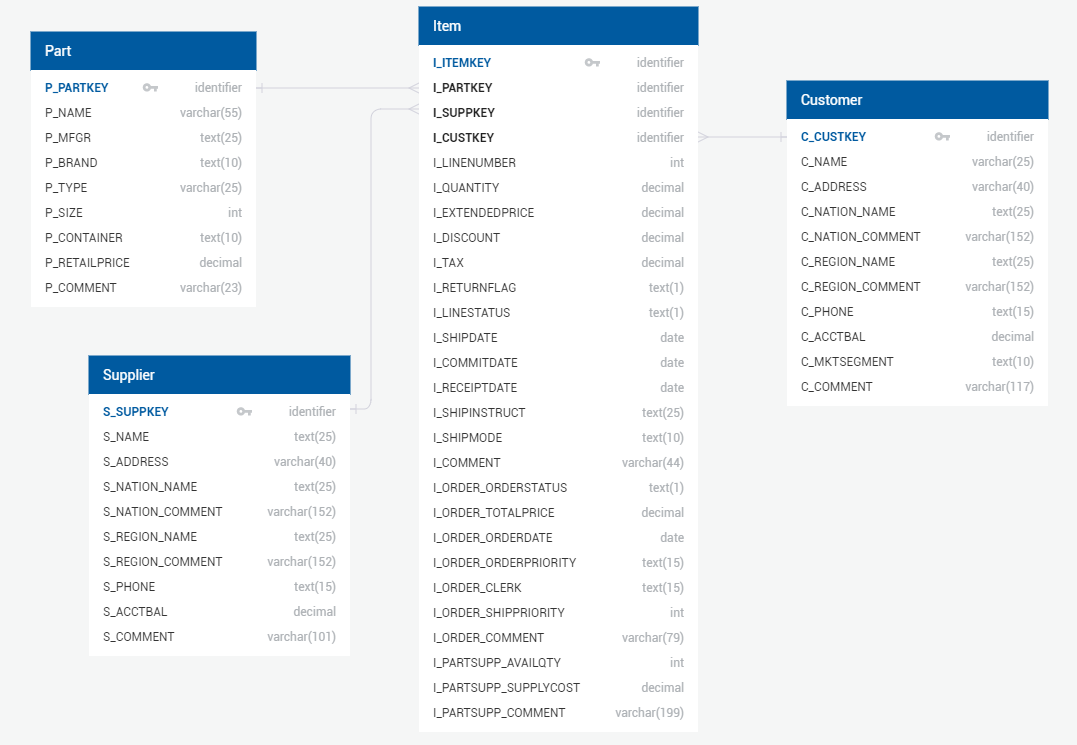
\includegraphics[width=\textwidth]{img/star.png}
	\caption{Esquema do ambiente desnormalizado}
	\label{fig:star}
\end{figure*}
 
A primeira modificação no modelo \textit{Snow Flake} foi a exclusão das entidades Dimensão \textit{Nation} e \textit{Region}. Essas entidades são Tabelas Subdimensionais das entidades \textit{Customer} e \textit{Supplier}, sendo frequentemente requeridas quando há a necessidade de consultar a nação e/ou a região de um cliente e/ou de um fornecedor, assim optou-se por incluir os atributos \texttt{N\_NAME, N\_COMMENT, R\_NAME} e \texttt{R\_COMMENT} nas entidades \textit{Supplier} e \textit{Customer}. 

Com a intenção de criar uma única Tabela Fato no esquema desnormalizado, observou-se (i) a possibilidade de unir as entidades \textit{Lineitem} e \textit{Orders} em uma única entidade nomeada como \textit{Item}, visto que as duas possuem um relacionamento. Isto também eliminaria alguns \textit{joins} realizados entre as duas entidades nas consultas listadas no Apêndice \ref{queries_1}. A PK \texttt{C\_CUSTKEY} de \textit{Customer} que antes estava em \textit{Orders} como FK é transferida agora para \textit{Item}. Também nota-se que (ii) as entidades \textit{Part} e \textit{Supplier} têm suas PKs como FKs na entidade antes denominada \textit{Lineitem}, provenientes da entidade intermediária \textit{Partsupp}. Optou-se assim por incluir os atributos de \textit{Partsupp} na nova entidade \textit{Item}, excluindo a primeira do esquema e mantendo o relacionamento de \textit{Supplier} e \textit{Part} diretamente com \textit{Item}, através das chaves \texttt{P\_PARTKEY} e \texttt{S\_SUPPKEY}.

O esquema final agora possui uma Tabela Fato, \textit{Item}; e três tabelas Dimensão, \textit{Part}, \textit{Customer} e \textit{Supplier}, cada qual com sua chave mantendo o relacionamento com a tabela \textit{Item}. Os dados presentes nas entidades são do mesmo tipo descritos na Seção \ref{ambiente_1}. As consultas em Linguagem SQL relacionadas a esse ambiente são encontradas no Apêndice \ref{queries_2}.

A inserção dos dados do Ambiente Desnormalizado será realizada após todos os dados gerados pelo DBGen do Ambiente Normalizado terem sido populados nos SGBDs. Com isso, é possível realizar \textit{joins} de acordo com as mudanças e o resultado destes será armazenado no esquema correspondente. Por exemplo, ao realizar um \textit{join} entre as entidades \textit{Nation} e \textit{Region} selecionando todos os seus atributos, estes são enviados como entrada para a inserção em uma nova tabela do esquema Desnormalizado correspondente, digamos, \textit{Nation\_Region}. Após, é realizado um novo \textit{join} com as entidades \textit{Supplier} e \textit{Part}, separadamente, para incluir os atributos de \textit{Nation\_Region}: \texttt{N\_NAME, N\_COMMENT, R\_NAME} e \texttt{R\_COMMENT}; bem como os atributos originais das duas entidades anteriores, nas novas entidades \textit{Supplier} e \textit{Part}.
\graphicspath{ {6-Experimento/} }

\chapter{O Experimento}

Como mencionado no Capítulo \ref{sgbd}, muitas empresas ainda utilizam 
bancos relacionais como forma de gerenciar seus dados. Existem vários SGBDR 
atuantes no mercado, como MySQL, PostgreSQL e algumas variantes da Oracle. 
Por se tratar de um SGBD \textit{open source} e ser amplamente 
conhecido, foi escolhido para o estudo o PostgreSQL. Ele possui vasta 
documentação, tutoriais e suporte em fóruns sobre bancos de dados e 
programação de forma geral, além de receber recorrentes atualizações. 

A categoria de NoSQL escolhida foi a colunar, por ser a mais 
recomendada para gerenciamento do grande volume de dados de um DW. 
O fato do PostgreSQL utilizar a Linguagem SQL como forma de 
manipulação de dados faz com que seja necessário também escolher 
o banco colunar para comparação utilizando esse filtro. A escolha também 
se deu com base na simplicidade do uso do SGBD, e na praticidade de 
migração dos dados armazenados entre um banco e outro. Para tanto, 
o MonetDB foi definido para o estudo.

O gerenciamento dos SGBD foi realizado através do \textit{driver} JDBC 
disponibilizados nas páginas oficiais do PostgreSQL e do MonetDB. Seu uso se deu 
devido à simplificação no desenvolvimento de aplicações, por dar suporte a 
diferentes SGBD e possuir boa documentação e tutoriais. Na análise de tempo 
foi considerada a latência da Máquina Virtual Java (JVM), assim incluindo essa 
latência no tempo total. As versões dos SGBD utilizadas 
foram o PostgreSQL 9.6 e o MonetDB 11.29.3 e foram instalados no servidor do laboratório GIA, operando sob o 
sistema operacional Ubuntu Linux 16.04 LTS, com 16Gb de RAM e dois 
processadores Intel Xeon CPU E5620 2.40GHz.

Os cenários de teste consistiram de três bases de dados de tamanhos 
diferentes, de 1Gb, 10Gb e 30Gb para simular desde uma base pequena 
até bases maiores. Cada cenário foi executado nos ambientes \textit{snowflake} e 
\textit{star}.

Alguns fatores devem ser considerados ao executar testes de \textit{benchmark} 
no escopo de banco de dados \cite{raasveldt2018fair}:

\begin{enumerate}
    \item{O ambiente de execução 
    deve ser o mesmo para todos os SGBD, bem como a lógica e sequência de 
    execução.}
    \item{A modelagem do banco deve ser idêntica para todos os modelos, e isso 
    inclui os tipos de dados e restrições de integridade. Ao analisar os resultados do \textit{benchmark}, a menos 
    que seja especificado no estudo, não há como saber qual é o tipo de dado de um atributo 
    quando existem diferentes tipos que podem ser usados para a mesma função, 
    e essa diferença acarreta em resultados diferentes de desempenho. Por exemplo, 
    em Raasveldt et al. \cite{raasveldt2018fair} o SGBD MariaDB apresentou diferenças quando implementado 
    utilizando DECIMAL e DOUBLE.}
    \item{\textit{Cold run} vs. \textit{Hot run}: em alguns sistemas a primeira execução de 
    testes (\textit{cold}) costuma levar mais tempo para executar que as execuções subsequentes (\textit{hot}). 
    Isso se dá pelo buffer do banco de dados ou o próprio sistema operacional ter armazenado em 
    cache os dados requeridos.}
\end{enumerate}

Os itens 1 e 2 foram tratados antes da execução do TPC-H. Nos Apêndices \ref{ddl_snow} e \ref{ddl_star} se encontram as SQL 
utilizadas para criar os esquemas \textit{snowflake} e \textit{star} nos SGBD. O fluxograma da Figura \ref{fig:flux} 
ilustra ainda a sequência de passos desde a criação dos bancos até a execução do \textit{benchmark}. 

O item 3 foi tratado durante a execução das consultas do teste de força: para cada cenário é realizada três 
análises diferentes, a primeira considerando a primeira execução de consultas; a segunda considerando o melhor 
resultado entre três execuções; e a terceira limpando parte da cache do sistema operacional antes de 
rodar a terceira execução. Essa análise é feita somente sob as consultas do teste de força por ser o primeiro 
teste a ser feito, como pode ser observado na Figura \ref{fig:power_flux}, que ilustra o fluxograma do teste de força. No teste de vazão todas as consultas já foram executadas 
uma vez e as funções de atualização trabalham sobre dados diferentes a cada vez que são executadas, impossibilitando 
o armazenamento em cache.

\begin{figure*}[htpb]
	\centering
        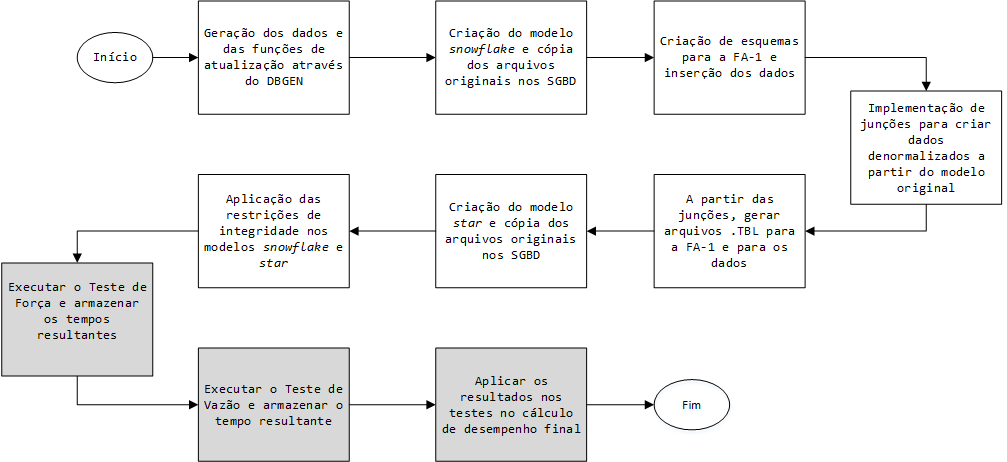
\includegraphics[width=\textwidth]{flux}
	\caption{Fluxograma do desenvolvimento até o cálculo final de desempenho do TPC-H}
	\label{fig:flux}
\end{figure*}

\begin{figure*}[htpb]
	\centering
        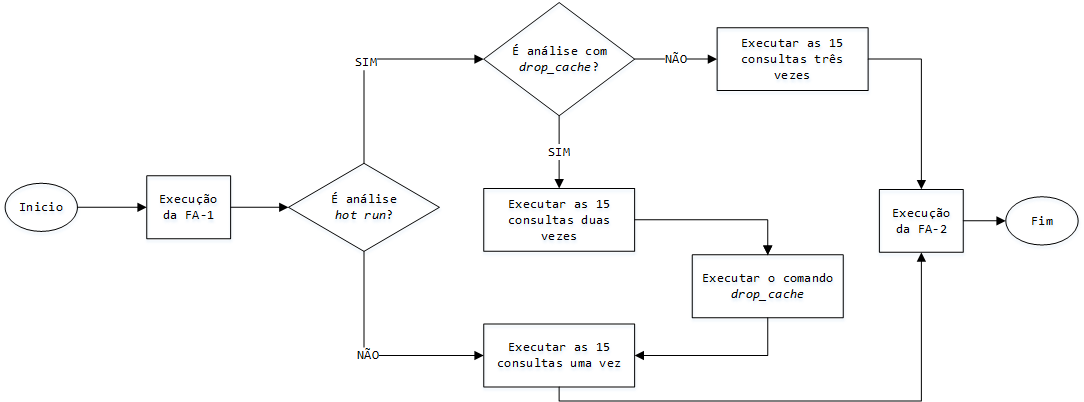
\includegraphics[width=\textwidth]{power_flux}
	\caption{Fluxograma do desenvolvimento do teste de força considerando todas as variações de cenário}
	\label{fig:power_flux}
\end{figure*}

Para averiguar se todas as 22 consultas do TPC-H executam de forma correta e em tempo hábil, principalmente 
atentando-se ao fato de que no ambiente denormalizado elas foram modificadas, foi realizada uma execução 
prévia de cada uma, sob a menor base de dados, utilizando o JDBC. Dessa execução, foram eliminadas as consultas 
Q1, Q2, Q4, Q15, Q17, Q20 e Q21 por terem demorado horas no ambiente denormalizado -- e algumas tendo a execução 
cancelada antes -- enquanto que as demais levaram apenas alguns segundos para executar. Essa mudança no número 
de consultas fez com que as equações originais fossem adaptadas para a nova quantidade, 15.

\begin{myequation}%
\label{eq:1-2}
{\scriptstyle Power@Size} = \frac{3600 * SF}{\sqrt[17]{\prod_{i = 1}^{i = 15}Q(i, 0) * \prod_{j = 1}^{j = 2}RF(j, 0)}} %
\end{myequation}
%

\begin{myequation}%
\label{eq:2-2}
{\scriptstyle Throughput@Size} = \frac{S * 15 * 3600}{T_s * SF} %
\end{myequation}
%

\section{Carregamento de Dados}

Após gerar todos os arquivos contendo os registros para inserção nos SGBD, foi utilizando o comando \textit{COPY}. Para se obter um melhor desempenho na inserção de dados as restrições de chaves foram aplicadas após a inserção de todos os dados. Caso a restrição fosse feita na criação do banco a cada novo registro inserido a chave primária seria verificada. Esta carga de dados também foi realizada através dos SGBD de forma direta, sem o uso de \textit{drivers} e outras ferramentas que possam atuar como cliente para conectar-se ao banco, assim evitando incluir o tempo de latência destas no resultado. Os comandos no MonetDB e no PostgreSQL são, respectivamente:

\begin{verbatim}
COPY INTO tabela FROM arquivo USING DELIMITERS delimitadores;
COPY tabela FROM arquivo DELIMITER delimitadores;
\end{verbatim}

A Tabela \ref{tab:carregamento} mostra o tempo em segundos para a inserção de dados nos SGBD. Logo ao analisar os resultados de carregamento de dados nota-se que um banco denormalizado apresenta certa demora na inserção de dados em relação a um normalizado. Isso se dá por causa da redundância de dados existente neste tipo de modelo, fazendo com que existam mais atributos duplicados em uma mesma entidade; aumentando o tamanho das entidades a serem inseridas. 

\begin{table}[htpb]
        \centering
        \caption{Tempo de carregamento em segundos para os cenários de \textit{benchmark}}
        \label{tab:carregamento}
        \begin{tabular}{c|ccc|c}
        \hline
        \multirow{2}{*}{SGBD} & \multicolumn{3}{c|}{Base de Dados (Gb)} & \multirow{2}{*}{Ambiente}  \\
                              & 1           & 10          & 30          &                            \\ \hline
        MonetDB               & 44          & 409         & 1351        & \multirow{2}{*}{\textit{Snowflake}} \\
        PostgreSQL            & 104         & 816         & 4979        &                            \\ \hline
        MonetDB               & 88          & 689         & 2216        & \multirow{2}{*}{\textit{Star}}      \\
        PostgreSQL            & 166         & 2365        & 7216        &                            \\ \hline
        \end{tabular}
    \end{table}

Toma-se como exemplo a entidade \textit{nation}: no modelo \textit{snowflake} ela é uma tabela subdimensão e possui 25 registros apenas, enquanto que no modelo denormalizado ela faz parte das tabelas dimensão \textit{supplier} e \textit{customer}, fazendo com que estas duas entidades tenham mais bytes armazenados. A Tabela \ref{tab:tamanho} mostra o tamanho dos arquivos gerados para cada modelo para a base de dados de 1Gb. Note que \textit{part} não tem seu valor alterado por não sofrer alteração entre as modelagens.

\begin{table}[htpb]
\centering
\caption{Tamanho em bytes das entidades}
\label{tab:tamanho}
\begin{tabular}{@{}lcc@{}}
\toprule
              & Snowflake & Star       \\ \midrule
Supplier      & 1.409.184   & 2.990.430    \\
Customer      & 24.346.144  & 48.055.517   \\
Part          & 24.135.125  & 24.135.125   \\
Lineitem/Item & 759.863.287 & 2.226.620.122 \\ \bottomrule
\end{tabular}
\end{table}

Um ponto importante a ser analisado foi o tamanho final de cada SGBD. A Tabela \ref{tab:carregamento_size} 
mostra que mesmo para a mesma quantidade de dados o MonetDB tem o tamanho em bytes reduzido, mostrando a capacidade 
que um SGBD colunar tem de realizar compressão de dados de forma mais eficiente.

\begin{table}[htpb]
    \centering
    \caption{Tamanho do banco de dados em Mb para os cenários de \textit{benchmark}}
    \label{tab:carregamento_size}
    \begin{tabular}{c|ccc|c}
        \hline
        \multirow{2}{*}{SGBD} & \multicolumn{3}{c|}{Base de Dados (Gb)} & \multirow{2}{*}{Ambiente}  \\
                              & 1           & 10          & 30          &                            \\ \hline
        MonetDB               & 771         & 8087        & 21352       & \multirow{2}{*}{\textit{Snowflake}} \\
        PostgreSQL            & 1567        & 15510       & 44371       &                            \\ \hline
        MonetDB               & 952         & 9352        & 26271       & \multirow{2}{*}{\textit{Star}}      \\
        PostgreSQL            & 2565        & 25487       & 71586       &                            \\ \hline
        \end{tabular}
    \end{table}

% -----------------------------
% COLD RUN

\section{Execução \textit{Cold Run}}

O primeiro cenário de execução consiste em analisar os resultados de desempenho considerando a primeira execução sequencial de todas as consultas do teste de força. 

\subsection{Base de Dados de 1Gb}

Considerando fator de escala de 1Gb, o número de registros das tabelas \textit{supplier, customer, part, partsupp, orders} e \textit{lineitem} são respectivamente 10.000, 150.000, 200.000, 800.000, 1.500.000 e 6.001.215. O número de registros das tabelas \textit{region} e \textit{nation} são fixos em 5 e 25, respectivamente. Também, em \textit{lineitem} o número de registros depende de um pedido em \textit{orders}, sendo definido sob um número aleatório entre um e quatro.

% TABELA DE TEMPO DE CONSULTAS E RF
\begin{table}[htpb]
        \centering
        \caption{Tempo em segundos de todas as consultas do teste de força e funções de atualização sob \textit{cold run} para 1Gb}
        \label{tab:queries_cold_1}
        \begin{tabular}{|c|c|c|c|c|}
        \hline
        & \multicolumn{2}{c|}{\textit{\textbf{Snowflake}}} & \multicolumn{2}{c|}{\textit{\textbf{Star}}} \\ \hline
        \textbf{SGBD}  & \textbf{MonetDB}      & \textbf{PostgreSQL}      & \textbf{MonetDB}    & \textbf{PostgreSQL}   \\ \hline
        \textbf{RF-1}  & 2.742             & 49.125              & 2.975          & 45.889            \\ \hline
        \textbf{Q3}    & 9.094             & 13.615              & 18.056         & 65.649            \\ \hline
        \textbf{Q5}    & 0.985             & 2.673               & 1.877          & 3.851             \\ \hline
        \textbf{Q6}    & 1.846             & 3.365               & 2.053          & 2.779             \\ \hline
        \textbf{Q7}    & 0.892             & 1.648               & 1.324          & 2.913             \\ \hline
        \textbf{Q8}    & 1.256             & 2.685               & 2.341          & 5.132             \\ \hline
        \textbf{Q9}    & 3.485             & 5.870               & 3.867          & 5.375             \\ \hline
        \textbf{Q10}   & 0.983             & 2.975               & 1.468          & 3.427             \\ \hline
        \textbf{Q11}   & 0.356             & 0.503               & 2.224          & 7.608             \\ \hline
        \textbf{Q12}   & 2.199             & 2.958               & 2.853          & 3.097             \\ \hline
        \textbf{Q13}   & 2.502             & 2.639               & 11.019         & 12.157            \\ \hline
        \textbf{Q14}   & 0.129             & 2.012               & 0.266          & 2.691             \\ \hline
        \textbf{Q16}   & 0.617             & 1.626               & 1.766          & 9.761             \\ \hline
        \textbf{Q18}   & 1.613             & 6.968               & 1.280          & 15.757            \\ \hline
        \textbf{Q19}   & 0.646             & 2.578               & 0.922          & 3.508             \\ \hline
        \textbf{Q22}   & 0.323             & 0.979               & 0.967          & 4.738             \\ \hline
        \textbf{Total} & 26.925            & 53.092              & 52.285         & 148.443           \\ \hline
        \textbf{RF-2}  & 40.812            & 38.091              & 20.260         & 20.575            \\ \hline
        \end{tabular}
        \end{table}

% TABELA DE POWER E VAZÃO
O primeiro conjunto de resultados para a execução de 1Gb pode ser visto nas Tabelas \ref{tab:queries_cold_1} e \ref{tab:forca_vazao_cold_1}. A primeira mostra os tempos em segundos que os dois SGBD levaram para executar as RF e as 15 consultas. Nela é possível verificar que a primeira consulta (Q3) é a que mais consome tempo de execução, e que o MonetDB não tem desempenho melhor que o PostgreSQL na remoção de registros no ambiente \textit{snowflake}, e ao contrário do que se esperava, este SGBD em ambiente denormalizado levou mais tempo para processar as consultas ao normalizado. 

Na Tabela \ref{tab:forca_vazao_cold_1} é possível perceber que o SGBD que obteve resultados dentro do esperado foi o PostgreSQL. O desempenho considerando um único usuário ativo foi melhor no ambiente normalizado, assim como no teste simulando vários usuários ativos. O MonetDB só alcançou resultados melhores no ambiente denormalizado para o último teste.

\begin{table}[htpb]
        \centering
        \caption{Valores do teste de força e vazão sob \textit{cold run} para 1Gb}
        \label{tab:forca_vazao_cold_1}
        \begin{tabular}{|c|c|c|c|c|}
        \hline
                                & \multicolumn{2}{c|}{\textbf{Teste de Força}} & \multicolumn{2}{c|}{\textbf{Teste de Vazão}} \\ \hline
        \textbf{SGBD}      & \textbf{MonetDB}    & \textbf{PostgreSQL}    & \textbf{MonetDB}    & \textbf{PostgreSQL}    \\ \hline
        \textbf{Snowflake} & 2541.636            & 980.630                & 1622.929            & 958.028                \\ \hline
        \textbf{Star}      & 1504.254            & 501.254                & 2468.020            & 637.310                \\ \hline
        \end{tabular}
\end{table}

% ---------------------------------
% BASE DE 10 GB

\subsection{Base de Dados de 10Gb}

\begin{table}[htpb]
        \centering
        \caption{Tempo em segundos de todas as consultas do teste de força e funções de atualização sob \textit{cold run} para 10Gb}
        \label{tab:queries_cold_10}
        \begin{tabular}{|c|c|c|c|c|}
        \hline
                & \multicolumn{2}{c|}{\textit{\textbf{Snowflake}}} & \multicolumn{2}{c|}{\textit{\textbf{Star}}} \\ \hline
        \textbf{SGBD}  & \textbf{MonetDB}      & \textbf{PostgreSQL}      & \textbf{MonetDB}    & \textbf{PostgreSQL}   \\ \hline
        \textbf{RF-1}  & 14.351                & 1304.641                 & 12.596              & 1042.060              \\ \hline
        \textbf{Q3}    & 125.044               & 108.010                  & 164.697             & 194.322               \\ \hline
        \textbf{Q5}    & 8.762                 & 37.100                   & 10.069              & 192.718               \\ \hline
        \textbf{Q6}    & 18.130                & 19.793                   & 13.621              & 155.163               \\ \hline
        \textbf{Q7}    & 2.913                 & 28.333                   & 0.327               & 151.504               \\ \hline
        \textbf{Q8}    & 9.072                 & 25.755                   & 9.396               & 151.010               \\ \hline
        \textbf{Q9}    & 18.126                & 93.686                   & 14.613              & 209.017               \\ \hline
        \textbf{Q10}   & 5.551                 & 46.611                   & 5.347               & 137.693               \\ \hline
        \textbf{Q11}   & 3.416                 & 10.951                   & 15.150              & 261.915               \\ \hline
        \textbf{Q12}   & 15.206                & 29.331                   & 20.039              & 129.920               \\ \hline
        \textbf{Q13}   & 19.837                & 35.913                   & 43.488              & 256.449               \\ \hline
        \textbf{Q14}   & 0.443                 & 19.775                   & 2.696               & 132.184               \\ \hline
        \textbf{Q16}   & 4.251                 & 14.154                   & 14.163              & 225.790               \\ \hline
        \textbf{Q18}   & 8.330                 & 137.693                  & 8.901               & 349.738               \\ \hline
        \textbf{Q19}   & 4.347                 & 25.855                   & 2.962               & 134.205               \\ \hline
        \textbf{Q22}   & 2.367                 & 14.979                   & 8.144               & 234.272               \\ \hline
        \textbf{Total} & 245.795               & 647.938                  & 333.613             & 2915.899              \\ \hline
        \textbf{RF-2}  & 526.547               & 379.049                  & 157.183             & 196.822               \\ \hline

\end{tabular}
\end{table}

O número de registros das tabelas \textit{supplier, customer, part, partsupp} e \textit{orders} correspondem aos valores da base de 1Gb, porém 10 vezes maior -- exceto \textit{lineitem}, cujo valor é 59.986.052. São respectivamente 100.000, 1.500.000, 2.000.000, 8.000.000, 15.000.000.

Nesta execução fica evidente a diferença de tempo da primeira consulta para as demais no banco colunar. Tomando a segunda mais lenta no MonetDB normalizado e denormalizado (Q13), a Q3 é 6.3 vezes no primeiro ambiente, e quase quatro vezes no segundo, mais demorada. Ainda, o ambiente denormalizado continua tendo desempenho pior que o normalizado no MonetDB, como é possível verificar na Tabela \ref{tab:queries_cold_10}. A Tabela \ref{tab:forca_vazao_cold_10} continua apresentando a mesma lógica que a Tabela \ref{tab:forca_vazao_cold_1} nos resultados.

\begin{table}[htpb]
        \centering
        \caption{Valores do teste de força e vazão sob \textit{cold run} para 10Gb}
        \label{tab:forca_vazao_cold_10}
        \begin{tabular}{|c|c|c|c|c|}
        \hline
                                & \multicolumn{2}{c|}{\textbf{Teste de Força}} & \multicolumn{2}{c|}{\textbf{Teste de Vazão}} \\ \hline
        \textbf{SGBD}      & \textbf{MonetDB}    & \textbf{PostgreSQL}    & \textbf{MonetDB}    & \textbf{PostgreSQL}    \\ \hline
        \textbf{Snowflake} & 3687.621            & 775.652                & 330.479             & 364.541                \\ \hline
        \textbf{Star}      & 3116.068            & 174.381                & 583.560             & 149.455                \\ \hline
        \end{tabular}
\end{table}


\subsection{Base de Dados de 30Gb}

O número de registros das tabelas \textit{supplier, customer, part, partsupp} e \textit{orders} correspondem aos valores da base de 1Gb, porém 30 vezes maior. São respectivamente 300.000, 4.500.000, 6.000.000, 24.000.000, 45.000.000, e \textit{lineitem} tem agora 179.998.372 registros.

Pela Tabela \ref{tab:queries_cold_30} pode-se verificar que no banco colunar o comportamento permanece o mesmo às bases anteriores. Desta vez ainda a escalabilidade do tempo da consulta Q14 aumentou em 208 vezes em comparação à base de 1Gb no ambiente normalizado e 334 vezes no denormalizado, enquanto que as demais consultas escalaram em um intervalo de valores com menos discrepâncias, ficando entre 13 e 75, e 12 e 69. Os resultados do teste de força e vazão são apresentados na Tabela \ref{tab:forca_vazao_cold_30}.

\begin{table}[htpb]
        \centering
        \caption{Valores do teste de força e vazão sob \textit{cold run} para 30Gb}
        \label{tab:forca_vazao_cold_30}
        \begin{tabular}{|c|c|c|c|c|}
        \hline
                                & \multicolumn{2}{c|}{\textbf{Teste de Força}} & \multicolumn{2}{c|}{\textbf{Teste de Vazão}} \\ \hline
        \textbf{SGBD}      & \textbf{MonetDB}    & \textbf{PostgreSQL}    & \textbf{MonetDB}    & \textbf{PostgreSQL}    \\ \hline
        \textbf{Snowflake} & 2329.918            & 369.019                & 112.572             & 220.005                \\ \hline
        \textbf{Star}      & 1474.766            & 145.064                & 165.419             & 120.578                \\ \hline
        \end{tabular}
\end{table}

\begin{table}[t]
        \centering
        \caption{Tempo em segundos de todas as consultas do teste de força e funções de atualização sob \textit{cold run} para 30Gb}
        \label{tab:queries_cold_30}
        \begin{tabular}{|c|c|c|c|c|}
        \hline
                & \multicolumn{2}{c|}{\textit{\textbf{Snowflake}}} & \multicolumn{2}{c|}{\textit{\textbf{Star}}} \\ \hline
        \textbf{SGBD}  & \textbf{MonetDB}      & \textbf{PostgreSQL}      & \textbf{MonetDB}    & \textbf{PostgreSQL}   \\ \hline
        \textbf{RF-1}  & 45.464                & 4346.899                 & 29.397              & 4011.410              \\ \hline
        \textbf{Q3}    & 250.579               & 369.306                  & 507.637             & 566.055               \\ \hline
        \textbf{Q5}    & 43.135                & 415.032                  & 79.365              & 581.650               \\ \hline
        \textbf{Q6}    & 87.109                & 203.049                  & 70.875              & 525.149               \\ \hline
        \textbf{Q7}    & 12.287                & 302.879                  & 24.758              & 542.459               \\ \hline
        \textbf{Q8}    & 24.375                & 286.555                  & 45.394              & 545.627               \\ \hline
        \textbf{Q9}    & 104.949               & 597.415                  & 54.817              & 717.576               \\ \hline
        \textbf{Q10}   & 14.495                & 296.734                  & 19.087              & 545.421               \\ \hline
        \textbf{Q11}   & 9.308                 & 50.995                   & 68.687              & 1073.476              \\ \hline
        \textbf{Q12}   & 96.438                & 260.277                  & 79.686              & 531.999               \\ \hline
        \textbf{Q13}   & 62.886                & 124.179                  & 194.227             & 937.462               \\ \hline
        \textbf{Q14}   & 26.823                & 219.780                  & 89.018              & 549.628               \\ \hline
        \textbf{Q16}   & 11.826                & 74.054                   & 68.930              & 834.195               \\ \hline
        \textbf{Q18}   & 109.423               & 796.233                  & 88.697              & 1225.532              \\ \hline
        \textbf{Q19}   & 48.729                & 191.799                  & 46.524              & 482.566               \\ \hline
        \textbf{Q22}   & 8.121                 & 88.714                   & 25.656              & 969.976               \\ \hline
        \textbf{Total} & 910.485               & 4277.000                 & 1463.358            & 10628.772             \\ \hline
        \textbf{RF-2}  & 1392.401              & 1120.928                 & 735.083             & 586.293               \\ \hline

\end{tabular}
\end{table}


\subsection{Desempenho Geral}

No cenário rodando sob \textit{cold run} o MonetDB não obteve resultados considerados estáveis como o PostgreSQL. Embora haja a conclusão que o SGBD colunar é melhor que o relacional, avaliando os dados dentro do MonetDB não se sabe ao certo qual modelagem é melhor, trazendo incerteza na sua escolha. 

Considerando vários usuários ativos o resultado foi como esperado. Se considerar também somente as RF, o MonetDB teve valores muito superiores para inserção de dados, e na remoção somente para uma base maior no ambiente denormalizado o PostgreSQL foi melhor. O que impactou nos resultados do banco colunar foi o comportamento anormal das consultas.

O comportamento do teste de força no banco MonetDB não segue uma queda conforme a base de dados aumenta. Existe uma inflexão na base de dados de 10Gb, pois não há um comportamento similar entre as consultas como acontece no PostgreSQL. Os gráficos das Figuras \ref{fig:power_snow_cold} e \ref{fig:power_star_cold} evidenciam isso. 

\begin{figure*}[htpb]
        \centering
        \subfigure[]{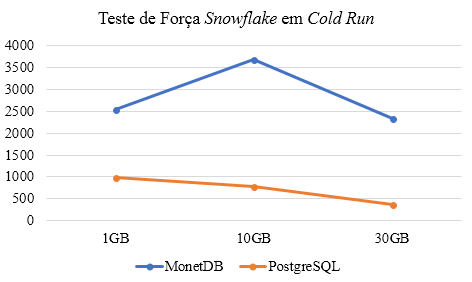
\includegraphics[width=7.2cm]{power_snow_cold}\label{fig:power_snow_cold}}
        \subfigure[]{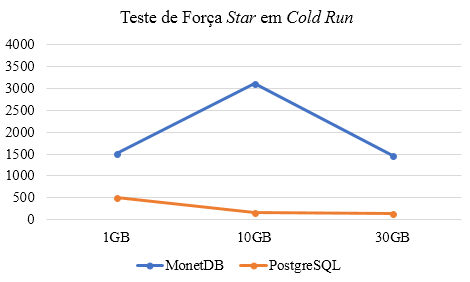
\includegraphics[width=7.2cm]{power_star_cold}\label{fig:power_star_cold}}
        \caption{Gráficos de força entre ambientes sob \textit{cold run}}
        \label{fig:power_cold}
\end{figure*}

O cálculo de desempenho final foi afetado por essa inflexão. Se analisar os resultados considerando os SGBD sob as modelagens \textit{snowflake} e \textit{star}, o MonetDB se destaca no resultado final, fazendo dele a melhor escolha entre os bancos, como mostram os gráficos da Figuras \ref{fig:qph_snow_cold} e \ref{fig:qph_star_cold} e os ganhos obtidos por ele em relação ao PostgreSQL conforme a Tabela \ref{tab:ganho_monet_psql_cold}. Porém ao considerar os ambientes sob cada SGBD, a única conclusão coerente que se tem é de que o PostgreSQL é melhor em ambientes normalizados, como ilustra o gráfico da Figura \ref{fig:qph_psql_cold}, no qual conforme a base aumenta o cálculo de desempenho é menor e sempre há ganhos do normalizado em relação ao denormalizado, sendo estes \textbf{42\%, 70\%} e \textbf{54\%} para 1Gb, 10Gb e 30Gb respectivamente.

\begin{figure*}[htpb]
        \centering
        \subfigure[]{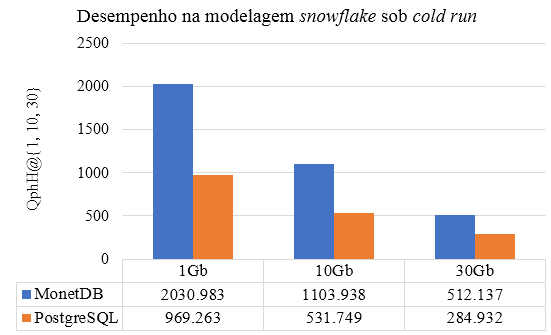
\includegraphics[width=7.2cm]{qph_snow_cold}\label{fig:qph_snow_cold}}
        \subfigure[]{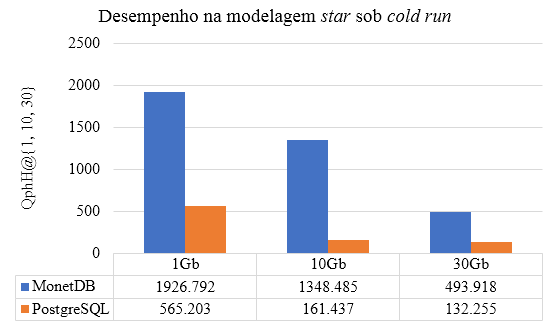
\includegraphics[width=7.2cm]{qph_star_cold}\label{fig:qph_star_cold}}
        \caption{Gráficos de desempenho entre ambientes sob \textit{cold run}}
        \label{fig:qph_model_cold}
\end{figure*}

\begin{table}[htpb]
        \centering
        \caption{Porcentagem de ganho de desempenho do MonetDB em relação ao PostgreSQL sob \textit{cold run}}
        \label{tab:ganho_monet_psql_cold}
        \begin{tabular}{|c|c|c|c|}
        \hline
        \multirow{2}{*}{\textbf{Ambiente}} & \multicolumn{3}{c|}{\textbf{Base de Dados (Gb)}} \\ \cline{2-4} 
                                           & \textbf{1}     & \textbf{10}    & \textbf{30}    \\ \hline
        \textit{Snowflake}                 & 110\%          & 108\%          & 80\%           \\ \hline
        \textit{Star}                      & 241\%          & 735\%          & 273\%          \\ \hline
        \end{tabular}
\end{table}

\begin{figure*}[htpb]
        \centering
        \subfigure[]{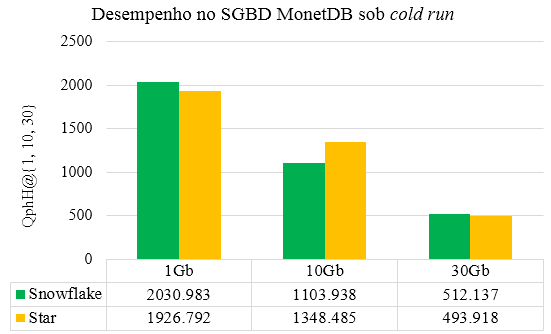
\includegraphics[width=7.2cm]{qph_monet_cold}\label{fig:qph_monet_cold}}
        \subfigure[]{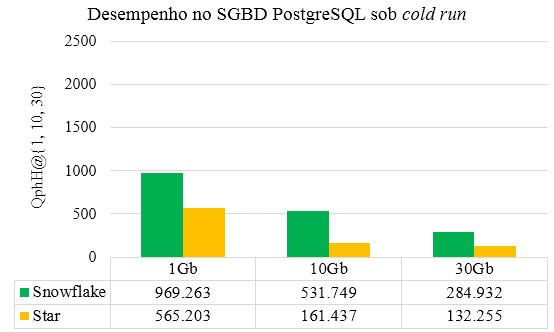
\includegraphics[width=7.2cm]{qph_psql_cold}\label{fig:qph_psql_cold}}
        \caption{Gráficos de desempenho entre SGBD sob \textit{cold run}}
        \label{fig:qph_sgbd_cold}
\end{figure*}

O MonetDB não segue uma lógica da qual se pode tirar alguma conclusão de acordo com a modelagem. Conforme o tamanho da base de dados aumenta o valor diminui assim como no PostgreSQL, porém entre as modelagens há uma inconsistência na comparação entre seus valores, visto que para 1Gb o ambiente normalizado foi melhor com ganho de \textbf{5\%}, já para 10Gb foi o denormalizado com \textbf{22\%} de ganho, e para 30Gb o comportamento é como em 1Gb com \textbf{4\%} de ganho do normalizado, como ilustra o gráfico da Figura \ref{fig:qph_monet_cold}. 

% --------------------------------------------
% HOT RUN

\section{Execução \textit{Hot Run}}

O segundo cenário de execução analisa os resultados de desempenho considerando a terceira execução sequencial de todas as consultas do teste de força, sendo esta executada imediatamente após as duas primeiras. O objetivo é verificar se há diferença nos resultados encontrados no cenário anterior. Os registros e a quantidade são os mesmos dos cenários anteriores. 

\subsection{Base de Dados de 1Gb}

Na terceira execução de todas as consultas já nota-se uma grande diferença nos valores do MonetDB, tanto no ambiente normalizado quanto no denormalizado. A primeira consulta já não é a mais lenta, e todas as demais têm valores similares considerando que a base de dados é pequena, como mostra a Tabela \ref{tab:queries_hot_1}. Percebe-se também que agora o ambiente denormalizado não é mais lento que o normalizado. Este resultado impacta nos valores de força, visto que pode-se analisar a partir da Tabela \ref{tab:forca_vazao_hot_1} que agora o ambiente \textit{star} tem valor superior ao \textit{snowflake} no MonetDB. Não apenas superior, os valores resultantes do teste de força possuem magnitude maior que os do cenário anterior devido a eficiência do processamento das consultas.

% TABELA DE POWER E VAZÃO

\begin{table}[htpb]
        \centering
        \caption{Valores do teste de força e vazão sob \textit{hot run} para 1Gb}
        \label{tab:forca_vazao_hot_1}
        \begin{tabular}{|c|c|c|c|c|}
        \hline
                                & \multicolumn{2}{c|}{\textbf{Teste de Força}} & \multicolumn{2}{c|}{\textbf{Teste de Vazão}} \\ \hline
        \textbf{SGBD}      & \textbf{MonetDB}    & \textbf{PostgreSQL}    & \textbf{MonetDB}    & \textbf{PostgreSQL}    \\ \hline
        \textit{\textbf{Snowflake}} & 14043.395           & 1222.570               & 1622.929            & 958.028                \\ \hline
        \textit{\textbf{Star}}      & 21811.705           & 659.758                & 2468.020            & 637.310                \\ \hline
        \end{tabular}
\end{table}

% TABELA DE TEMPO DE CONSULTAS E RF
\begin{table}[htpb]
        \centering
        \caption{Tempo em segundos de todas as consultas do teste de força e funções de atualização sob \textit{hot run} para 1Gb}
        \label{tab:queries_hot_1}
        \begin{tabular}{|c|c|c|c|c|}
        \hline
        & \multicolumn{2}{c|}{\textit{\textbf{Snowflake}}} & \multicolumn{2}{c|}{\textit{\textbf{Star}}} \\ \hline
        \textbf{SGBD}  & \textbf{MonetDB}      & \textbf{PostgreSQL}      & \textbf{MonetDB}    & \textbf{PostgreSQL}   \\ \hline
        \textbf{RF-1}  & 2.742             & 49.125              & 2.975            & 45.889              \\ \hline
        \textbf{Q3}    & 0.184             & 1.874               & 0.079            & 3.231               \\ \hline
        \textbf{Q5}    & 0.116             & 1.165               & 0.063            & 3.303               \\ \hline
        \textbf{Q6}    & 0.047             & 2.126               & 0.051            & 2.762               \\ \hline
        \textbf{Q7}    & 0.149             & 1.611               & 0.067            & 2.796               \\ \hline
        \textbf{Q8}    & 0.519             & 2.178               & 0.078            & 3.344               \\ \hline
        \textbf{Q9}    & 0.301             & 5.004               & 0.089            & 5.187               \\ \hline
        \textbf{Q10}   & 0.090             & 2.703               & 0.049            & 3.381               \\ \hline
        \textbf{Q11}   & 0.099             & 0.499               & 0.102            & 7.510               \\ \hline
        \textbf{Q12}   & 0.161             & 2.955               & 0.070            & 3.085               \\ \hline
        \textbf{Q13}   & 0.155             & 2.609               & 0.092            & 12.106              \\ \hline
        \textbf{Q14}   & 0.050             & 2.008               & 0.060            & 2.593               \\ \hline
        \textbf{Q16}   & 0.383             & 1.708               & 0.667            & 9.359               \\ \hline
        \textbf{Q18}   & 0.768             & 6.949               & 0.508            & 8.970               \\ \hline
        \textbf{Q19}   & 0.140             & 2.553               & 0.121            & 3.204               \\ \hline
        \textbf{Q22}   & 0.073             & 0.973               & 0.090            & 3.777               \\ \hline
        \textbf{Total} & 3.236             & 36.918              & 2.184            & 74.606              \\ \hline
        \textbf{RF-2}  & 40.812            & 38.091              & 20.260           & 20.575              \\ \hline
        \end{tabular}
        \end{table}


% ---------------------------------
% BASE DE 10 GB

\subsection{Base de Dados de 10Gb}

Assim como a base de dados de 1Gb, a de 10Gb possui um comportamento que trazem resultados melhores que no cenário considerando \textit{cold run}, e novamente o MonetDB apresentou valores mais consistentes, e o ambiente denormalizado apresentou resultados melhores que o normalizado.

\begin{table}[htpb]
        \centering
        \caption{Valores do teste de força e vazão sob \textit{hot run} para 10Gb}
        \label{tab:forca_vazao_hot_10}
        \begin{tabular}{|c|c|c|c|c|}
        \hline
        & \multicolumn{2}{c|}{\textbf{Teste de Força}} & \multicolumn{2}{c|}{\textbf{Teste de Vazão}} \\ \hline
        \textbf{SGBD}               & \textbf{MonetDB}    & \textbf{PostgreSQL}    & \textbf{MonetDB}    & \textbf{PostgreSQL}    \\ \hline
        \textit{\textbf{Snowflake}} & 11861.997           & 870.994                & 330.479             & 364.541                \\ \hline
        \textit{\textbf{Star}}      & 17902.155           & 190.307                & 583.560             & 149.455                \\ \hline
        \end{tabular}
\end{table}

\begin{table}[t]
        \centering
        \caption{Tempo em segundos de todas as consultas do teste de força e funções de atualização sob \textit{hot run} para 10Gb}
        \label{tab:queries_hot_10}
        \begin{tabular}{|c|c|c|c|c|}
        \hline
                & \multicolumn{2}{c|}{\textit{\textbf{Snowflake}}} & \multicolumn{2}{c|}{\textit{\textbf{Star}}} \\ \hline
        \textbf{SGBD}  & \textbf{MonetDB}      & \textbf{PostgreSQL}      & \textbf{MonetDB}    & \textbf{PostgreSQL}   \\ \hline
        \textbf{RF-1}  & 14.351            & 1304.641            & 12.596           & 1042.060            \\ \hline
        \textbf{Q3}    & 2.118             & 36.095              & 1.506            & 125.089             \\ \hline
        \textbf{Q5}    & 1.171             & 34.593              & 1.273            & 159.875             \\ \hline
        \textbf{Q6}    & 0.438             & 19.789              & 0.602            & 132.427             \\ \hline
        \textbf{Q7}    & 2.679             & 28.960              & 1.277            & 146.097             \\ \hline
        \textbf{Q8}    & 6.416             & 24.142              & 1.428            & 126.529             \\ \hline
        \textbf{Q9}    & 3.004             & 107.818             & 0.597            & 170.805             \\ \hline
        \textbf{Q10}   & 1.324             & 35.949              & 0.223            & 128.092             \\ \hline
        \textbf{Q11}   & 2.515             & 5.494               & 0.686            & 263.927             \\ \hline
        \textbf{Q12}   & 3.649             & 29.372              & 1.505            & 122.578             \\ \hline
        \textbf{Q13}   & 6.173             & 31.265              & 8.303            & 261.873             \\ \hline
        \textbf{Q14}   & 0.390             & 18.737              & 0.161            & 132.393             \\ \hline
        \textbf{Q16}   & 1.161             & 14.239              & 6.757            & 225.479             \\ \hline
        \textbf{Q18}   & 8.136             & 125.887             & 5.643            & 339.079             \\ \hline
        \textbf{Q19}   & 2.356             & 26.911              & 1.801            & 125.114             \\ \hline
        \textbf{Q22}   & 0.570             & 19.855              & 2.736            & 215.812             \\ \hline
        \textbf{Total} & 42.100            & 559.107             & 34.498           & 2675.167            \\ \hline
        \textbf{RF-2}  & 526.547           & 379.049             & 157.183          & 196.822             \\ \hline
        \end{tabular}
\end{table}

\subsection{Base de Dados de 30Gb}

Para a base de 30Gb além de manter-se o comportamento das anteriores, percebe-se um distanciamento maior dos valores do MonetDB para o PostgreSQL em \textit{hot run}. Os valores da Tabela \ref{tab:queries_hot_30} mostram isso e a Tabela \ref{tab:forca_vazao_hot_30} apresenta os valores de força e vazão.

\begin{table}[htpb]
        \centering
        \caption{Valores do teste de força e vazão sob \textit{hot run} para 30Gb}
        \label{tab:forca_vazao_hot_30}
        \begin{tabular}{|c|c|c|c|c|}
        \hline
                                & \multicolumn{2}{c|}{\textbf{Teste de Força}} & \multicolumn{2}{c|}{\textbf{Teste de Vazão}} \\ \hline
        \textbf{SGBD}      & \textbf{MonetDB}    & \textbf{PostgreSQL}    & \textbf{MonetDB}    & \textbf{PostgreSQL}    \\ \hline
        \textit{\textbf{Snowflake}} & 5457.325            & 363.441                & 112.572             & 220.005                \\ \hline
        \textit{\textbf{Star}}      & 6873.122            & 149.514                & 165.419             & 120.578                \\ \hline
        \end{tabular}
\end{table}

\begin{table}[t]
        \centering
        \caption{Tempo em segundos de todas as consultas do teste de força e funções de atualização sob \textit{hot run} para 30Gb}
        \label{tab:queries_hot_30}
        \begin{tabular}{|c|c|c|c|c|}
        \hline
                & \multicolumn{2}{c|}{\textit{\textbf{Snowflake}}} & \multicolumn{2}{c|}{\textit{\textbf{Star}}} \\ \hline
        \textbf{SGBD}  & \textbf{MonetDB}      & \textbf{PostgreSQL}      & \textbf{MonetDB}    & \textbf{PostgreSQL}   \\ \hline
        \textbf{RF-1}  & 45.464            & 4346.899            & 29.397           & 4011.410            \\ \hline
        \textbf{Q3}    & 68.066            & 329.075             & 57.567           & 553.795             \\ \hline
        \textbf{Q5}    & 12.812            & 373.031             & 12.553           & 537.089             \\ \hline
        \textbf{Q6}    & 2.579             & 186.510             & 1.608            & 473.006             \\ \hline
        \textbf{Q7}    & 3.086             & 279.495             & 1.487            & 501.833             \\ \hline
        \textbf{Q8}    & 6.984             & 281.131             & 6.220            & 507.657             \\ \hline
        \textbf{Q9}    & 60.413            & 607.088             & 30.875           & 671.788             \\ \hline
        \textbf{Q10}   & 11.154            & 310.681             & 9.409            & 518.880             \\ \hline
        \textbf{Q11}   & 9.597             & 68.390              & 9.784            & 980.716             \\ \hline
        \textbf{Q12}   & 42.212            & 261.946             & 40.280           & 476.657             \\ \hline
        \textbf{Q13}   & 62.234            & 144.715             & 56.124           & 916.111             \\ \hline
        \textbf{Q14}   & 1.576             & 224.288             & 1.297            & 551.986             \\ \hline
        \textbf{Q16}   & 11.634            & 75.528              & 13.937           & 835.383             \\ \hline
        \textbf{Q18}   & 56.660            & 771.133             & 49.197           & 1224.231            \\ \hline
        \textbf{Q19}   & 28.730            & 186.968             & 27.263           & 495.281             \\ \hline
        \textbf{Q22}   & 7.037             & 104.941             & 6.001            & 1127.978            \\ \hline
        \textbf{Total} & 384.775           & 4204.921            & 323.601          & 10372.392           \\ \hline
        \textbf{RF-2}  & 1392.401          & 1120.928            & 735.083          & 586.293             \\ \hline
        \end{tabular}
\end{table}

\subsection{Desempenho Geral}

Ao contrário do cenário sob \textit{cold run}, utilizar o terceiro conjunto de consultas trouxe estabilidade nos valores das consultas do teste de força no MonetDB. Isso fez com que a inflexão que antes acontecia não acontecesse mais, podendo agora encontrar uma lógica na análise dos ambientes considerando o SGBD. As Figuras \ref{fig:power_snow_hot} e \ref{fig:power_star_hot} apresentam os gráficos do teste de força, agora apresentando queda nos valores conforme a base de dados aumenta.

\begin{figure*}[htpb]
        \centering
        \subfigure[]{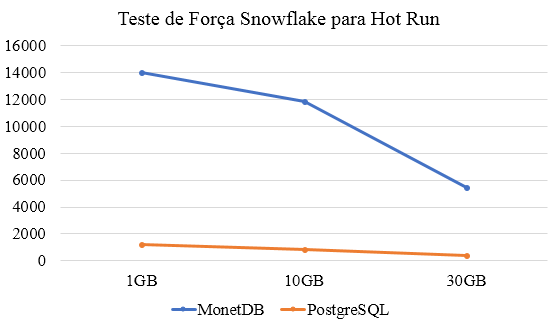
\includegraphics[width=7.2cm]{power_snow_hot}\label{fig:power_snow_hot}}
        \subfigure[]{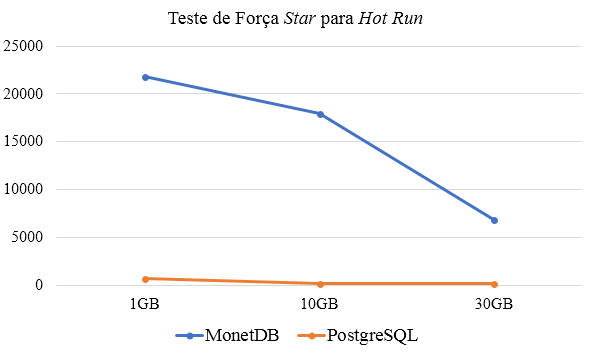
\includegraphics[width=7.2cm]{power_star_hot}\label{fig:power_star_hot}}
        \caption{Gráficos de força entre ambientes sob \textit{hot run}}
        \label{fig:power_hot}
\end{figure*}

Pelo gráfico das Figuras \ref{fig:qph_snow_hot} e \ref{fig:qph_star_hot} percebe-se que o MonetDB continua melhor que o PostgreSQL, conforme os ganhos apresentados na Tabela \ref{tab:ganho_monet_psql_hot}, e agora seus valores também são superiores aos calculados no desempenho final considerando a \textit{cold run}. Ainda, analisando os ambientes sob cada SGBD pelos gráficos das Figuras \ref{fig:qph_monet_hot} e \ref{fig:qph_psql_hot} nota-se pela segunda que o PostgreSQL continua tendo desempenho melhor no ambiente normalizado ao denormalizado, com ganhos de \textbf{40\%, 70\%} e \textbf{53\%} enquanto que a primeira mostra que agora o MonetDB possui valores superiores em todas as bases para o ambiente denormalizado, com ganhos de \textbf{54\%, 63\%} e \textbf{63\%}.

\begin{figure*}[htpb]
        \centering
        \subfigure[]{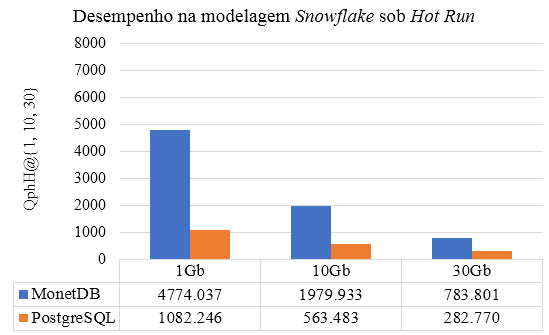
\includegraphics[width=7.2cm]{qph_snow_hot}\label{fig:qph_snow_hot}}
        \subfigure[]{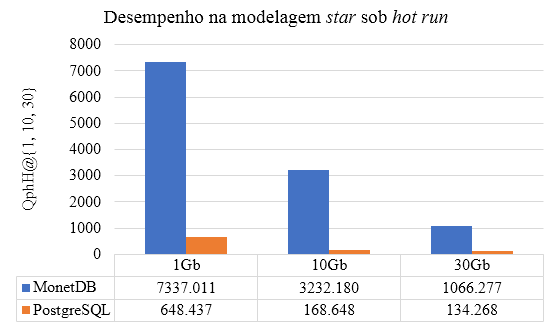
\includegraphics[width=7.2cm]{qph_star_hot}\label{fig:qph_star_hot}}
        \caption{Gráficos de desempenho entre ambientes sob \textit{hot run}}
        \label{fig:qph_model_hot}
\end{figure*}

\begin{table}[htpb]
        \centering
        \caption{Porcentagem de ganho de desempenho do MonetDB em relação ao PostgreSQL sob \textit{hot run}}
        \label{tab:ganho_monet_psql_hot}
        \begin{tabular}{|c|c|c|c|}
        \hline
        \multirow{2}{*}{\textbf{Ambiente}} & \multicolumn{3}{c|}{\textbf{Base de Dados (Gb)}} \\ \cline{2-4} 
        & \textbf{1}     & \textbf{10}    & \textbf{30}    \\ \hline
        \textit{Snowflake}                 & 341\%          & 251\%          & 177\%          \\ \hline
        \textit{Star}                      & 1031\%         & 1817\%         & 694\%          \\ \hline
        \end{tabular}
\end{table}
    
\begin{figure*}[htpb]
        \centering
        \subfigure[]{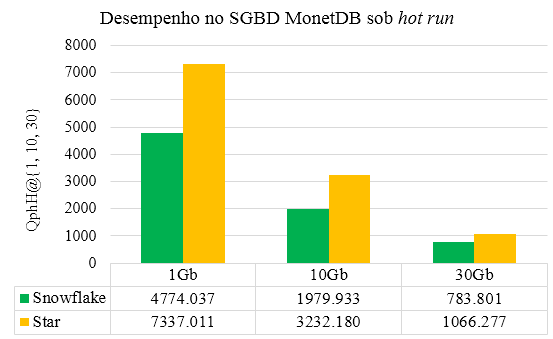
\includegraphics[width=7.2cm]{qph_monet_hot}\label{fig:qph_monet_hot}}
        \subfigure[]{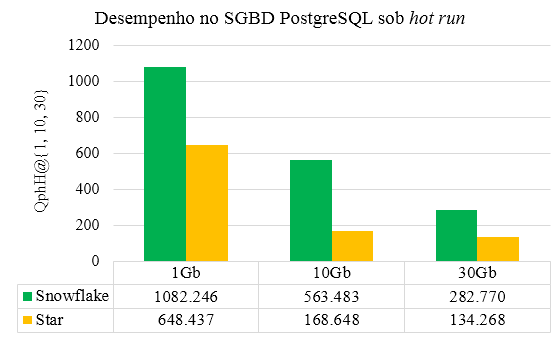
\includegraphics[width=7.2cm]{qph_psql_hot}\label{fig:qph_psql_hot}}
        \caption{Gráficos de desempenho entre SGBD sob \textit{hot run}}
        \label{fig:qph_sgbd_hot}
\end{figure*}

Os valores do SGBD PostgreSQL não tiveram mudanças drásticas se comparar as execuções \textit{cold} e \textit{hot}, inclusive na base de dados 30Gb sob a modelagem normalizada a primeira foi melhor que a segunda. A Tabela \ref{tab:ganho_postgresql_cold_hot} mostra a porcentagem de ganho e perdas entre os valores obtidos na terceira execução em relação à primeira execução para o PostgreSQL. Entretanto, os valores do MonetDB se alteraram de forma que houve impacto no resultado final tanto do teste de força como no cálculo final de \textit{benchmark}, como mostram os ganhos da \textit{hot run} em relação à \textit{cold run} na Tabela \ref{tab:ganho_monet_cold_hot}.

\begin{table}[htpb]
        \centering
        \caption{Porcentagem de ganho e perda de desempenho do PostgreSQL da \textit{hot run} em relação à \textit{cold run}}
        \label{tab:ganho_postgresql_cold_hot}
        \begin{tabular}{|c|c|c|c|}
        \hline
        \multirow{2}{*}{\textbf{Ambiente}} & \multicolumn{3}{c|}{\textbf{Base de Dados (Gb)}} \\ \cline{2-4} 
        & \textbf{1}     & \textbf{10}    & \textbf{30}    \\ \hline
        \textit{Snowflake}                 & 10\%           & 6\%            & -1\%           \\ \hline
        \textit{Star}                      & 13\%           & 4\%            & 1\%            \\ \hline
        \end{tabular}
\end{table}

\begin{table}[htpb]
        \centering
        \caption{Porcentagem de ganho de desempenho do MonetDB da \textit{hot run} em relação à \textit{cold run}}
        \label{tab:ganho_monet_cold_hot}
        \begin{tabular}{|c|c|c|c|}
        \hline
        \multirow{2}{*}{\textbf{Ambiente}} & \multicolumn{3}{c|}{\textbf{Base de Dados (Gb)}} \\ \cline{2-4} 
        & \textbf{1}     & \textbf{10}    & \textbf{30}    \\ \hline
        \textit{Snowflake}                 & 57\%           & 44\%           & 35\%           \\ \hline
        \textit{Star}                      & 74\%           & 58\%           & 54\%           \\ \hline
        \end{tabular}
\end{table}

De acordo com a página oficial do MonetDB \cite{monetdb2017c}, este SGBD se destaca quando dados acessados pelo usuário podem ser mantidos na memória principal do servidor ou quando algumas colunas são solicitadas e são suficientes para manipular uma solicitação, como é o caso do ambiente analítico. Isso explica o porquê das consultas da primeira execução apresentarem desempenho inferior às da terceira execução. Na segunda e na terceira execução alguns dados das consultas já estão em \textit{cache}, assim o SGBD consegue recuperá-los mais rapidamente.

Dois exemplos que mostram a estabilidade nos valores alcançados pela \textit{cache} estão na primeira consulta (Q3) e na 11ª (Q14). No cenário de \textit{cold run} a primeira consulta sempre levava mais tempo que as demais e a Q14 demorava excessivamente conforme a base crescia, em detrimento das demais. Considerando este cenário uma justificativa a se utilizar seria a de que as consultas eram demoradas, porém sob o cenário \textit{hot run} se vê que elas não apresentam o mesmo comportamento, tendo influência da memória \textit{cache}.

\section{Execução com \textit{Drop Cache}}

O último cenário consiste em, levando em consideração que o MonetDB sofre influência da memória \textit{cache}, executar as consultas de força três vezes como no cenário anterior, porém antes da terceira execução efetuar a limpeza na memória \textit{cache} do sistema. A intenção é averiguar se os resultados serão alterados ao mudar o estado da \textit{cache}.

\subsection{Base de Dados de 1Gb}

O primeiro detalhe que se nota de acordo com os valores de tempo totais, em segundos, de cada execução de consultas é que a segunda execução é sempre a mais rápida devido a alguns valores já estarem armazenados em \textit{cache}. Após ter limpado parte da \textit{cache}, a terceira execução já torna-se mais lenta que a segunda, porém não mais que a primeira, pois alguns valores ainda podem ter ficado armazenados na memória.

\begin{table}[htpb]
        \centering
        \caption{Tempo total de execução das consultas da 1ª, 2ª e 3ª execução para 1Gb}
        \label{tab:queries_cache_1}
        \begin{tabular}{|c|c|c|c|c|}
        \hline
        SGBD       & 1ª Execução & 2ª Execução & 3ª Execução & Ambiente                            \\ \hline
        MonetDB    & 20.842      & 2.811       & 9.973       & \multirow{2}{*}{\textit{Snowflake}} \\ \cline{1-4}
        PostgreSQL & 77.689      & 37.906      & 54.328      &                                     \\ \hline
        MonetDB    & 54.197      & 3.082       & 26.147      & \multirow{2}{*}{\textit{Star}}      \\ \cline{1-4}
        PostgreSQL & 94.184      & 75.135      & 91.649      &                                     \\ \hline
        \end{tabular}
\end{table}

Dentre todas as consultas, a que mais sofreu impacto da oscilação da \textit{cache} foi a primeira. A Tabela \ref{tab:q1_cache_1} mostra os valores para a Q3 de todas as execuções.

\begin{table}[htpb]
        \centering
        \caption{Tempo total de execução da primeira consulta para 1Gb}
        \label{tab:q1_cache_1}
        \begin{tabular}{|c|c|c|c|c|}
        \hline
        SGBD       & 1ª Execução & 2ª Execução & 3ª Execução & Ambiente                            \\ \hline
        MonetDB    & 7.758       & 0.228       & 1.034       & \multirow{2}{*}{\textit{Snowflake}} \\ \cline{1-4}
        PostgreSQL & 36.574      & 1.855       & 13.698      &                                     \\ \hline
        MonetDB    & 18.345      & 0.071       & 9.656       & \multirow{2}{*}{\textit{Star}}      \\ \cline{1-4}
        PostgreSQL & 20.054      & 3.038       & 19.919      &                                     \\ \hline
\end{tabular}
\end{table}


\subsection{Base de Dados de 10Gb}

A mesma lógica da base de dados de 1Gb segue para a de 10Gb, segundo a Tabela \ref{tab:queries_cache_10}. Na execução do PostgreSQL em ambiente \textit{snowflake}, entretanto, houve uma queda no tempo de execução da segunda execução para a terceira, indicando possivelmente menor influência da \textit{cache} neste SGBD.


\begin{table}[htpb]
        \centering
        \caption{Tempo total de execução das consultas da 1ª, 2ª e 3ª execução para 10Gb}
        \label{tab:queries_cache_10}
        \begin{tabular}{|c|c|c|c|c|}
        \hline
        SGBD       & 1ª Execução & 2ª Execução & 3ª Execução & Ambiente                            \\ \hline
        MonetDB    & 412.301     & 31.825      & 90.525      & \multirow{2}{*}{\textit{Snowflake}} \\ \cline{1-4}
        PostgreSQL & 950.210     & 750.324     & 744.324     &                                     \\ \hline
        MonetDB    & 398.951     & 50.781      & 294.667     & \multirow{2}{*}{\textit{Star}}      \\ \cline{1-4}
        PostgreSQL & 3042.546    & 2772.970    & 2884.537    &                                     \\ \hline
        \end{tabular}
\end{table}

Nesta base já nota-se de forma acentual a influência da memória na primeira consulta como mostra a Tabela \ref{tab:q1_cache_10}, e consequentemente no resultado final de tempo de execução, podendo ocasionar a mesma inflexão apresentada pela primeira execução dos testes.

\begin{table}[htpb]
        \centering
        \caption{Tempo total de execução da primeira consulta para 10Gb}
        \label{tab:q1_cache_10}
        \begin{tabular}{|c|c|c|c|c|}
        \hline
        SGBD       & 1ª Execução & 2ª Execução & 3ª Execução & Ambiente                            \\ \hline
        MonetDB    & 273.352     & 2.460       & 11.734      & \multirow{2}{*}{\textit{Snowflake}} \\ \cline{1-4}
        PostgreSQL & 112.322     & 43.252      & 113.553     &                                     \\ \hline
        MonetDB    & 216.923     & 22.201      & 155.161     & \multirow{2}{*}{\textit{Star}}      \\ \cline{1-4}
        PostgreSQL & 200.664     & 149.393     & 218.902     &                                     \\ \hline
        \end{tabular}
\end{table}

\subsection{Base de Dados de 30Gb}

Assim como as anteriores, a Tabela \ref{tab:queries_cache_30} mostra que a terceira execução é afetada pela \textit{cache}, bem como a primeira consulta, cujos valores são mostrados na Tabela \ref{tab:q1_cache_30}.

\begin{table}[htpb]
        \centering
        \caption{Tempo total de execução das consultas da 1ª, 2ª e 3ª execução para 30Gb}
        \label{tab:queries_cache_30}
        \begin{tabular}{|c|c|c|c|c|}
        \hline
        SGBD       & 1ª Execução & 2ª Execução & 3ª Execução & Ambiente                            \\ \hline
        MonetDB    & 1062.709    & 495.334     & 688.593     & \multirow{2}{*}{\textit{Snowflake}} \\ \cline{1-4}
        PostgreSQL & 4574.974    & 4433.061    & 4300.868    &                                     \\ \hline
        MonetDB    & 1338.430    & 799.249     & 1243.989    & \multirow{2}{*}{\textit{Star}}      \\ \cline{1-4}
        PostgreSQL & 11128.495   & 10788.900   & 10884.908   &                                     \\ \hline
        \end{tabular}
\end{table}

\begin{table}[htpb]
        \centering
        \caption{Tempo total de execução da primeira consulta para 30Gb}
        \label{tab:q1_cache_30}
        \begin{tabular}{|c|c|c|c|c|}
        \hline
        SGBD       & 1ª Execução & 2ª Execução & 3ª Execução & Ambiente                            \\ \hline
        MonetDB    & 487.614     & 122.496     & 322.512     & \multirow{2}{*}{\textit{Snowflake}} \\ \cline{1-4}
        PostgreSQL & 381.837     & 353.038     & 361.421     &                                     \\ \hline
        MonetDB    & 517.566     & 146.583     & 465.564     & \multirow{2}{*}{\textit{Star}}      \\ \cline{1-4}
        PostgreSQL & 586.428     & 570.704     & 571.626     &                                     \\ \hline
        \end{tabular}
\end{table}

\subsection{Desempenho Geral}

As três subseções anteriores mostraram como a \textit{cache} influencia nos resultados do processamento das consultas, principalmente no SGBD MonetDB. Aplicando o cálculo do teste de força nos valores oriundos da terceira execução é observado a volta da inflexão na base de 10Gb, como mostram os gráficos das Figuras \ref{fig:power_snow_cache} e \ref{fig:power_star_cache}.

\begin{figure*}[htpb]
        \centering
        \subfigure[]{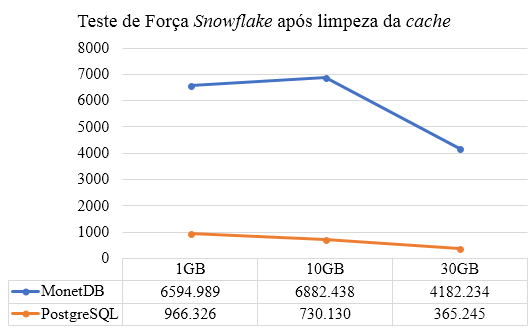
\includegraphics[width=7.2cm]{power_snow_cache}\label{fig:power_snow_cache}}
        \subfigure[]{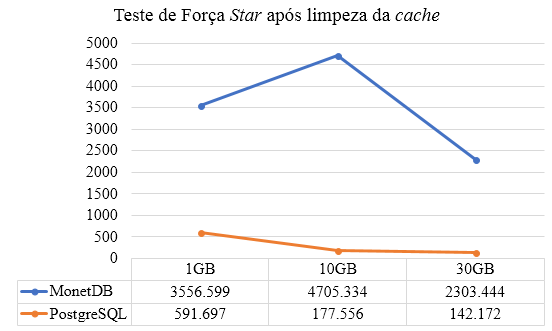
\includegraphics[width=7.2cm]{power_star_cache}\label{fig:power_star_cache}}
        \caption{Gráfico de força entre ambientes sob influência da limpeza de \textit{cache}}
        \label{fig:power_cache}
\end{figure*}

Para averiguar de fato essa influência da limpeza de \textit{cache} na inflexão, o mesmo teste de força foi aplicado nos valores de tempo da segunda execução, que já tinha alguns dados armazenados na memória. Os gráficos das Figuras \ref{fig:power_snow_cache_2} e \ref{fig:power_star_cache_2} ilustram que não ocorreu inflexão na segunda base de dados ao não limpar a \textit{cache}.

\begin{figure*}[htpb]
        \centering
        \subfigure[]{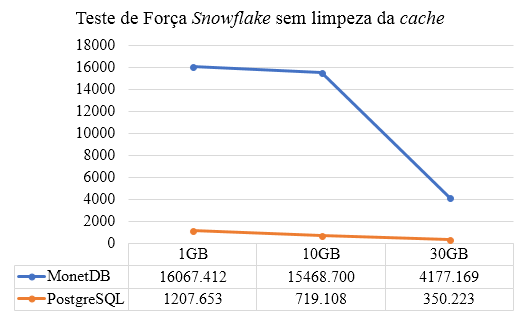
\includegraphics[width=7.2cm]{power_snow_cache_2}\label{fig:power_snow_cache_2}}
        \subfigure[]{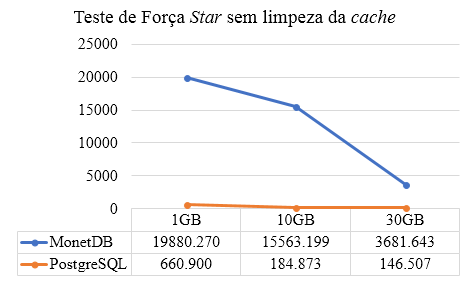
\includegraphics[width=7.2cm]{power_star_cache_2}\label{fig:power_star_cache_2}}
        \caption{Gráficos de força sem limpeza de \textit{cache}}
        \label{fig:power_cache_2}
\end{figure*}

A influência da inflexão pode ser vista na Figura \ref{fig:qph_monet_cache}, que assim como a Figura \ref{fig:qph_monet_cold} não apresenta conclusão acerca da escolha da modelagem para o banco MonetDB. A Figura \ref{fig:qph_psql_cache} mostra os valores finais entre os ambientes no PostgreSQL, e a Figura \ref{fig:qph_model_cache} os gráficos comparando os SGBD dentro de cada ambiente.
    
\begin{figure*}[htpb]
        \centering
        \subfigure[]{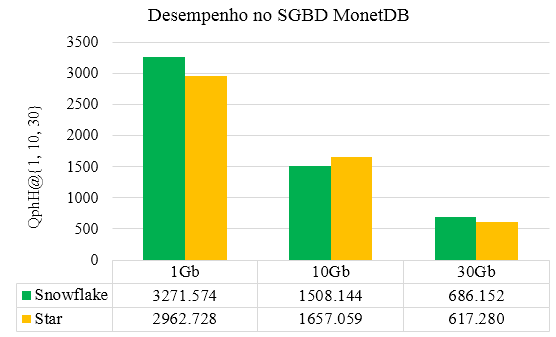
\includegraphics[width=7.2cm]{qph_monet_cache}\label{fig:qph_monet_cache}}
        \subfigure[]{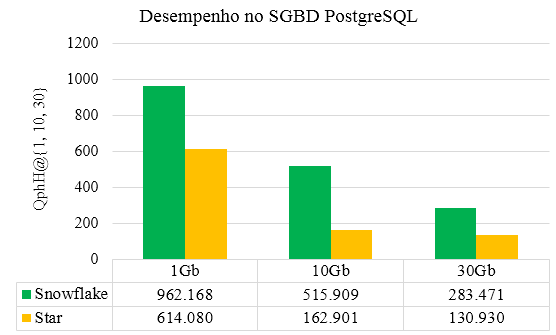
\includegraphics[width=7.2cm]{qph_psql_cache}\label{fig:qph_psql_cache}}
        \caption{Gráficos de desempenho entre SGBD sob influência da limpeza de \textit{cache}}
        \label{fig:qph_sgbd_cache}
\end{figure*}

Considerando a segunda execução, o resultado final de desempenho pode ser visto nos gráficos das Figuras \ref{fig:qph_model_cache_2} e \ref{fig:qph_sgbd_cache_2}. Nelas percebe-se a mesma lógica que as Figuras \ref{fig:qph_model_hot} e \ref{fig:qph_sgbd_hot} apresentam.

\begin{figure*}[htpb]
        \centering
        \subfigure[]{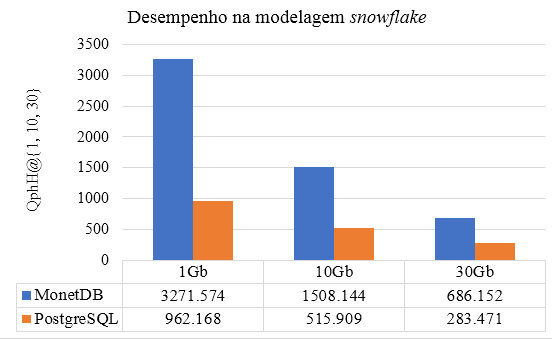
\includegraphics[width=7.2cm]{qph_snow_cache}\label{fig:qph_snow_cache}}
        \subfigure[]{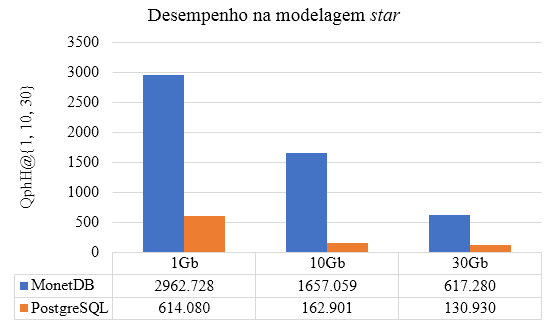
\includegraphics[width=7.2cm]{qph_star_cache}\label{fig:qph_star_cache}}
        \caption{Gráficos de desempenho entre ambientes sob influência da limpeza de \textit{cache}}
        \label{fig:qph_model_cache}
\end{figure*}

\begin{figure*}[t]
        \centering
        \subfigure[]{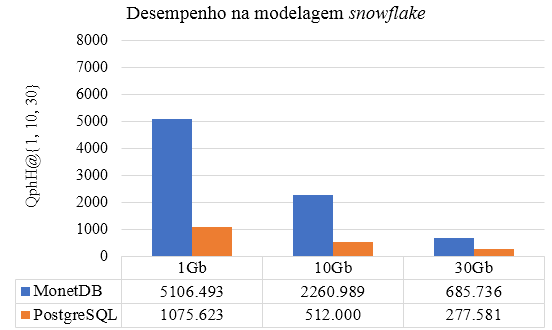
\includegraphics[width=7.2cm]{qph_snow_cache_2}\label{fig:qph_snow_cache_2}}
        \subfigure[]{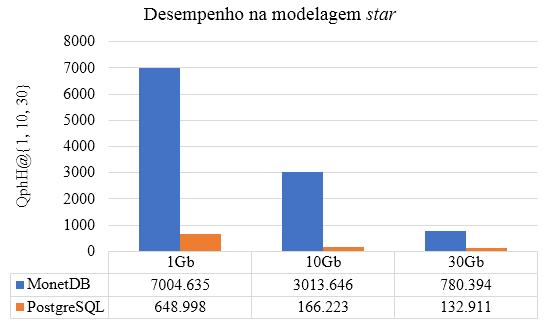
\includegraphics[width=7.2cm]{qph_star_cache_2}\label{fig:qph_star_cache_2}}
        \caption{Gráficos de desempenho entre ambientes sem limpeza de \textit{cache}}
        \label{fig:qph_model_cache_2}
\end{figure*}

\begin{figure*}[htpb]
        \centering
        \subfigure[]{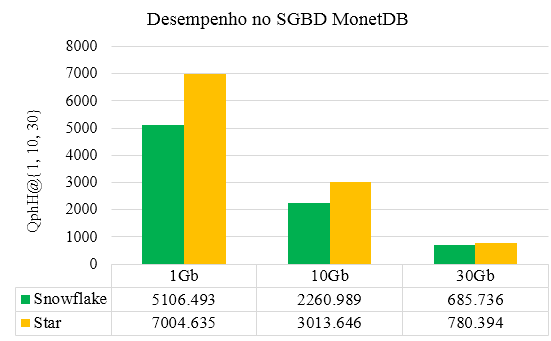
\includegraphics[width=7.2cm]{qph_monet_cache_2}\label{fig:qph_monet_cache_2}}
        \subfigure[]{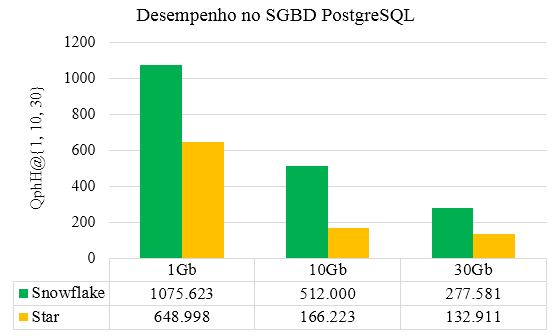
\includegraphics[width=7.2cm]{qph_psql_cache_2}\label{fig:qph_psql_cache_2}}
        \caption{Gráficos de desempenho entre SGBD sem limpeza de \textit{cache}}
        \label{fig:qph_sgbd_cache_2}
\end{figure*}

\chapter{Conclusões}

A principal discussão em um ambiente analítico é a necessidade por desempenho na recuperação de informações para tomada de decisão. Para conseguir alcançar de forma eficiente esse desempenho bancos relacionais são muito utilizados, porém podem trazer alguns problemas de acordo com a modelagem dos dados dos DWs. Para tanto, bancos de dados NoSQL, mais especificamente da classe orientada a colunas, ganham destaque por satisfazerem questões mais complexas em SGBD relacionais, tornando possível a recuperação rápida de dados.

Entre os destaques encontrados em um modelo de SGBD colunar estão (i) a capacidade de escalabilidade horizontal devido ao melhor desempenho sob modelagens denormalizadas no formato \textit{star}, o que faz com que não seja preciso normalizar um modelo a um nível que gere alto grau de acoplamento entre as tabelas do banco, (ii) busca dos atributos requeridos de forma direta, sem precisar processar tuplas inteiras, satisfazendo as requisições de consultas analíticas por poucos atributos, gerando rapidez na recuperação de dados, e (iii) alta capacidade de compressão de dados. Ao realizar a avaliação experimental os dois últimos pontos ficaram bem evidentes.

Desde a carga de dados nota-se uma grande diferença entre os SGBD MonetDB e PostgreSQL. O comando \textit{COPY INTO} utilizado pelo MonetDB consegue inserir os dados no SGBD concorrentemente -- um fator que o torna preferível ao invés de vários \textit{INSERT}, por tratar o comando como uma única \textit{query}\footnote{Aqui \textit{query} não significa exatamente uma \textit{consulta}, portanto optou-se por deixar a palavra no inglês por não encontrar uma tradução adequada} independentemente de ter o modo de \textit{auto-commit} das transações ativo ou não. Mesmo que o comando \textit{COPY FROM} do PostgreSQL assim como do MonetDB trate o comando como uma única \textit{query}, o mesmo desempenho não foi atingido. A Tabela \ref{tab:ganho_carregamento} mostra os ganhos do MonetDB em relação ao PostgreSQL no tempo de carregamento. Logo após a inserção de dados também percebe-se um grande diferencial dos bancos colunares: a compressão de dados, uma vez que o MonetDB realiza compressão de \textit{strings} utilizando codificação por dicionário.

\begin{table}[htpb]
    \centering
    \caption{Porcentagem de ganho de tempo de carregamento do MonetDB em relação ao PostgreSQL}
    \label{tab:ganho_carregamento}
    \begin{tabular}{|c|c|c|c|}
    \hline
    \multirow{2}{*}{\textbf{Ambiente}} & \multicolumn{3}{c|}{\textbf{Base de Dados (Gb)}} \\ \cline{2-4} 
                                       & \textbf{1}     & \textbf{10}    & \textbf{30}    \\ \hline
    \textit{Snowflake}                 & 58\%           & 50\%           & 73\%           \\ \hline
    \textit{Star}                      & 47\%           & 71\%           & 69\%           \\ \hline
    \end{tabular}
    \end{table}
    
Como um todo a teoria sobre SGBDR vs. SGBDC se aplicou bem à prática. O PostgreSQL teve um ótimo desempenho se comparar o ambiente mais normalizado ao denormalizado. Por ser desenvolvido visando modelos relacionais, o processamento de dados nas consultas tanto com uma quanto com várias \textit{streams} foi mais rápido no ambiente normalizado. Considerando vários usuários ativos o PostgreSQL conseguiu ser mais rápido que o MonetDB no ambiente normalizado para as bases de dados maiores (10Gb e 30Gb). Porém se analisar o desempenho final isso não fez com que o banco relacional pudesse ter desempenho melhor que o colunar no ambiente analítico.

Um fator que trouxe resultados melhores no MonetDB, além dos já citados de bancos colunares, foi o fato de que MonetDB faz uso intensivo de memória para processamento -- vale frisar que ele não requer que todos os dados caibam em toda memória física disponível, pois utiliza o espaço disponível em \textit{swap} e arquivos mapeados em memória. Devido a esse uso intensivo de memória, medir o tempo de uma consulta é algo delicado no MonetDB. Os testes comparando \textit{cold run}, \textit{hot run} e limpeza de \textit{cache} mostraram como a mesma consulta executada várias vezes e sob um cenário alterando a memória trazem resultados diferentes nesse SGBD, fazendo com que sob a primeira execução os resultados não acordem com a teoria descrita sobre o desempenho superior em ambientes \textit{star}.

Retomando a discussão entre OLAP e OLTP, armazenar os dados de um ambiente transacional em memória pode trazer problemas, tornando mais interessante de fato para um ambiente transacional que seus dados sejam armazenados em um dispositivo não-volátil. Um ambiente altamente normalizado perde por não escalar horizontalmente de forma tão simples, o que já acarreta demora na recuperação do servidor em caso de queda, portanto não é interessante que ocorra perda de dados em memória. Em um ambiente analítico, a inserção de dados já é mais rápida considerando o uso do MonetDB e ele pode ser escalável horizontalmente, fazendo com que uma queda e perda de dados em memória não seja tão crítica.

Para ambientes transacionais cuja modelagem ainda segue os padrões de normalização o uso de um SGBD como o PostgreSQL continua sendo vantajoso, pois além dos resultados obtidos deve se considerar que um SGBDR preza pela consistência nos dados, e para um sistema transacional que envolva transações bancárias, por exemplo, a consistência é fundamental. Em ambiente analítico é confirmado que um banco colunar traz melhor desempenho para a recuperação de informações e o MonetDB ainda possui a vantagem de utilizar dados em memória. Para que se faça um bom uso da \textit{cache} nesse SGBD é possível aproveitar justamente o fator de consultas analíticas, embora não idênticas, serem similares por simular cenários com agrupamentos e atributos Fato, para realizar um \textit{warm-up} de dados para que estes já estejam em \textit{cache}.

De maneira geral, a pesquisa corroborou a teoria de que SGBDR atuam melhor sob operações transacionais, e que mesmo em ambiente analítico a modelagem mais normalizada é ideal para esta classe de SGBD. Por não precisarem do mesmo desempenho para recuperação de informações como consultas analíticas, eles podem se ater a consistência de dados e a uma modelagem normalizada, optando por deixar de lado o particionamento horizontal dos dados, mesmo que isso degrade a disponibilidade destes ao ocorrer uma queda de servidor.

Para ambientes analíticos, reforça-se que um SGBDC é uma ótima escolha na recuperação de dados. Todos seus atributos estarão armazenados juntos, as chances de conseguir uma alta compressão são maiores e a reconstrução de tuplas, dependendo de qual for sua implementação, é feita de forma mais inteligente que em SGBDR. Por serem uma classe de SGBD NoSQL, garantem alta disponibilidade e são capazes de realizar particionamento horizontal, por isso o desempenho é melhor em modelagens denormalizadas, aumentando a eficiência na recuperação de dados em um DW.

% \section{Trabalhos Futuros}

Como continuidade para a pesquisa sugere-se:

\begin{itemize}
    \item Realizar um estudo mais aprofundado sobre escalabilidade horizontal em bancos NoSQL, e se possível aplicar o \textit{benchmark} considerando um cenário utilizando um único servidor para processamento de consultas e outro com vários servidores, a fim de simular problemas que teoricamente são solucionados pelo particionamento horizontal, como queda, ou falha, e distribuição de dados.

    \item Utilizar bases de dados maiores, a partir de 100Gb, para que se possa também comparar os resultados com os contidos na página oficial do TPC-H.

    \item Aplicar os resultados encontrados nesta pesquisa em empresas que ainda utilizem bancos relacionais ou, mesmo que usem outras alternativas, que ainda tenham uma modelagem normalizada, realizando a migração tanto do SGBD quanto da modelagem para um modelo colunar denormalizado.

    \item Comparar diferentes modelos colunares que, de preferência, trabalhem sob diferentes algoritmos de compressão, como o Cassandra \cite{cassandra2018nosql} e o C-Store \cite{cstore2018nosql}. Pode-se também incluir diferentes classes de NoSQL a fim de verificar se alguma consegue desempenho melhor que a classe colunar em ambiente analítico, como o MongoDB \cite{mongo2018nosql}.

\end{itemize}


% Como numerar os apêndices como inteiros
\appendix

% Inclus?o dos apêndices
\oneandhalfspacing
%============================================================

\chapter{Consultas do Ambiente Original Normalizado}
\label{queries_1}


São apresentadas aqui as 22 consultas do ambiente \textit{snowflake}, cada qual com sua questão de negócio brevemente explicada.

\begin{enumerate}

%--------------------------------------1
\item[Q1 --] Consulta de Relatório de Resumo de Preços \\
	Emite um relatório com o resumo de preços de todos os itens enviados em uma certa data. Esta data corresponde a 60-120 dias antes da maior data de envio contida no banco de dados. 
    
\begin{tabular}{ll}
	Parâmetro de Substituição & Valor\\
	DELTA & 90\\
\end{tabular}
    
	\begin{lstlisting}[language=SQL]
select
	l_returnflag,
	l_linestatus,
	sum(l_quantity) as sum_qty,
	sum(l_extendedprice) as sum_base_price,
	sum(l_extendedprice * (1 - l_discount)) as sum_disc_price,
	sum(l_extendedprice * (1 - l_discount) * (1 + l_tax)) as sum_charge,
	avg(l_quantity) as avg_qty,
	avg(l_extendedprice) as avg_price,
	avg(l_discount) as avg_disc,
	count(*) as count_order
from
	lineitem
where
	l_shipdate <= date '1998-12-01' - interval '[DELTA]' day (3)
group by
	l_returnflag,
	l_linestatus
order by
	l_returnflag,
	l_linestatus;
	
	\end{lstlisting}

% %--------------------------------------2
\item[Q2 --] Consulta de Fornecedor de Custo Mínimo

Encontra o fornecedor que pode fornecer um produto com o menor custo em uma dada região.
	
\begin{tabular}{ll}
	Parâmetro de Substituição & Valor\\
	SIZE & 15\\
	TYPE & BRASS\\
	REGION & EUROPE\\
\end{tabular}

	\begin{lstlisting}[language=SQL]
select
	s_acctbal,
	s_name,
	n_name,
	p_partkey,
	p_mfgr,
	s_address,
	s_phone,
	s_comment
from
	part,
	supplier,
	partsupp,
	nation,
	region
where
	p_partkey = ps_partkey
	and s_suppkey = ps_suppkey
	and p_size = [SIZE]
	and p_type like '%[TYPE]'
	and s_nationkey = n_nationkey
	and n_regionkey = r_regionkey
	and r_name = '[REGION]'
	and ps_supplycost = (
		select
			min(ps_supplycost)
		from
			partsupp,
			supplier,
			nation,
			region
		where
			p_partkey = ps_partkey
			and s_suppkey = ps_suppkey
			and s_nationkey = n_nationkey
			and n_regionkey = r_regionkey
			and r_name = '[REGION]'
	)
order by
	s_acctbal desc,
	n_name,
	s_name,
	p_partkey;
set rowcount 100
go
	\end{lstlisting}

%--------------------------------------3
\item[Q3 --] Consulta de Prioridade de Envio
	
	Retorna a prioridade de envio dos pedidos com a maior receita entre aqueles que ainda não foram enviados em uma determinada data.
	
\begin{tabular}{ll}
	Parâmetro de Substituição & Valor\\
	SEGMENT & BUILDING\\
	DATE & 1995-03-15\\
\end{tabular}

	\begin{lstlisting}[language=SQL]
select
	l_orderkey,
	sum(l_extendedprice * (1 - l_discount)) as revenue,
	o_orderdate,
	o_shippriority
from
	customer,
	orders,
	lineitem
where
	c_mktsegment = '[SEGMENT]'
	and c_custkey = o_custkey
	and l_orderkey = o_orderkey
	and o_orderdate < date '[DATE]'
	and l_shipdate > date '[DATE]'
group by
	l_orderkey,
	o_orderdate,
	o_shippriority
order by
	revenue desc,
	o_orderdate;
set rowcount 10
go
	\end{lstlisting}
	
%--------------------------------------4
\item[Q4 --] Consulta de Verificação de Prioridade de Pedido
		
	Faz a contagem do número de pedidos solicitados em um dado trimestre de um determinado ano no qual pelo menos um item foi recebido pelo cliente após a data de entrega.
	
\begin{tabular}{ll}
	Parâmetro de Substituição & Valor\\
	DATE & 1993-07-01\\
\end{tabular}

	\begin{lstlisting}[language=SQL]
select
	o_orderpriority,
	count(*) as order_count
from
	orders
where
	o_orderdate >= date '[DATE]'
	and o_orderdate < date '[DATE]' + interval '3' month
	and exists (
		select
			*
		from
			lineitem
		where
			l_orderkey = o_orderkey
			and l_commitdate < l_receiptdate
	)
group by
	o_orderpriority
order by
	o_orderpriority;
	
	\end{lstlisting}

%--------------------------------------5
\item[Q5 --] Consulta de Volume do Fornecedor Local
	
	Lista para cada nação em uma dada região o volume de receita originado de uma transação na qual cliente e fornecedor eram daquela nação.
	
\begin{tabular}{ll}
	Parâmetro de Substituição & Valor\\
	REGION & ASIA\\
	DATE & 1994-01-01\\
\end{tabular}

	\begin{lstlisting}[language=SQL]
select
	n_name,
	sum(l_extendedprice * (1 - l_discount)) as revenue
from
	customer,
	orders,
	lineitem,
	supplier,
	nation,
	region
where
	c_custkey = o_custkey
	and l_orderkey = o_orderkey
	and l_suppkey = s_suppkey
	and c_nationkey = s_nationkey
	and s_nationkey = n_nationkey
	and n_regionkey = r_regionkey
	and r_name = '[REGION]'
	and o_orderdate >= date '[DATE]'
	and o_orderdate < date '[DATE]' + interval '1' year
group by
	n_name
order by
	revenue desc;
	
	\end{lstlisting}
	
%--------------------------------------6
\item[Q6 --] Previsão de Mudança de Receita
	
	Informa o quanto a receita pode aumentar eliminando alguns descontos em um dado ano.
	
\begin{tabular}{ll}
	Parâmetro de Substituição & Valor\\
	DATE & 1994-01-01\\
	DISCOUNT & .06\\
	QUANTITY & 24\\
\end{tabular}

	\begin{lstlisting}[language=SQL]
select
	sum(l_extendedprice * l_discount) as revenue
from
	lineitem
where
	l_shipdate >= date '[DATE]'
	and l_shipdate < date '[DATE]' + interval '1' year
	and l_discount between [DISCOUNT] - 0.01 and [DISCOUNT] + 0.01
	and l_quantity < [QUANTITY];
	
	\end{lstlisting}
	
%--------------------------------------7
\item[Q7 --] Consulta de Quantidade de Envio

    Determina o valor de bens enviados entre nações para auxiliar na renegociação de contratos de envio.
    
\begin{tabular}{ll}
	Parâmetro de Substituição & Valor\\
	NATION1 & FRANCE\\
	NATION2 & GERMANY\\
\end{tabular}

	\begin{lstlisting}[language=SQL]
select
	supp_nation,
	cust_nation,
	l_year,
	sum(volume) as revenue
from
	(
		select
			n1.n_name as supp_nation,
			n2.n_name as cust_nation,
			extract(year from l_shipdate) as l_year,
			l_extendedprice * (1 - l_discount) as volume
		from
			supplier,
			lineitem,
			orders,
			customer,
			nation n1,
			nation n2
		where
			s_suppkey = l_suppkey
			and o_orderkey = l_orderkey
			and c_custkey = o_custkey
			and s_nationkey = n1.n_nationkey
			and c_nationkey = n2.n_nationkey
			and (
				(n1.n_name = '[NATION1]' and n2.n_name = '[NATION2]')
				or (n1.n_name = '[NATION2]' and n2.n_name = '[NATION1]')
			)
			and l_shipdate between date '1995-01-01' and date '1996-12-31'
	) as shipping
group by
	supp_nation,
	cust_nation,
	l_year
order by
	supp_nation,
	cust_nation,
	l_year;
	
	\end{lstlisting}

%--------------------------------------8
\item[Q8 --] Consulta de Quota de Mercado Nacional

    Determina quanto a quota de mercado de uma dada nação em uma dada região mudou em dois anos para um determinado tipo de peça.
    
\begin{tabular}{ll}
	Parâmetro de Substituição & Valor\\
	NATION & BRAZIL\\
	REGION & AMERICA\\
	TYPE &  ECONOMY ANODIZED STEEL\\
\end{tabular}

	\begin{lstlisting}[language=SQL]
select
	o_year,
	sum(case
		when nation = '[NATION]' 
		then volume
		else 0
	end) / sum(volume) as mkt_share
from
	(
		select
			extract(year from o_orderdate) as o_year,
			l_extendedprice * (1 - l_discount) as volume,
			n2.n_name as nation
		from
			part,
			supplier,
			lineitem,
			orders,
			customer,
			nation n1,
			nation n2,
			region
		where
			p_partkey = l_partkey
			and s_suppkey = l_suppkey
			and l_orderkey = o_orderkey
			and o_custkey = c_custkey
			and c_nationkey = n1.n_nationkey
			and n1.n_regionkey = r_regionkey
			and r_name = '[REGION]'
			and s_nationkey = n2.n_nationkey
			and o_orderdate between date '1995-01-01' and date '1996-12-31'
						and p_type = '[TYPE]'
	) as all_nations
group by
	o_year
order by
	o_year;
	
	\end{lstlisting}

%--------------------------------------9
\item[Q9 --] Consulta ao Lucro de um Tipo de Produto

    Encontra para cada nação em cada ano o lucro de todas as peças pedidas naquele ano contendo uma substring específica em seus nomes que foram preenchidos por um fornecedor naquela nação.
    
\begin{tabular}{ll}
	Parâmetro de Substituição & Valor\\
	COLOR & green\\
\end{tabular}

	\begin{lstlisting}[language=SQL]
select
	nation,
	o_year,
	sum(amount) as sum_profit
from
	(
		select
			n_name as nation,
			extract(year from o_orderdate) as o_year,
			l_extendedprice * (1 - l_discount) - ps_supplycost * l_quantity as a
mount
		from
			part,
			supplier,
			lineitem,
			partsupp,
			orders,
			nation
		where
			s_suppkey = l_suppkey
			and ps_suppkey = l_suppkey
			and ps_partkey = l_partkey
			and p_partkey = l_partkey
			and o_orderkey = l_orderkey
			and s_nationkey = n_nationkey
			and p_name like '%[COLOR]%'
	) as profit
group by
	nation,
	o_year
order by
	nation,
	o_year desc;
	
	\end{lstlisting}

%--------------------------------------10
\item[Q10 --] Consulta de Relatório de Itens Retornados

    Retorna os 20 principais clientes que podem estar tendo problemas com peças que foram enviadas a eles em um dado trimestre.
    
\begin{tabular}{ll}
	Parâmetro de Substituição & Valor\\
	DATE & 1993-10-01\\
\end{tabular}

	\begin{lstlisting}[language=SQL]
select
	c_custkey,
	c_name,
	sum(l_extendedprice * (1 - l_discount)) as revenue,
	c_acctbal,
	n_name,
	c_address,
	c_phone,
	c_comment
from
	customer,
	orders,
	lineitem,
	nation
where
	c_custkey = o_custkey
	and l_orderkey = o_orderkey
	and o_orderdate >= date '[DATE]'
	and o_orderdate < date '[DATE]' + interval '3' month
	and l_returnflag = 'R'
	and c_nationkey = n_nationkey
group by
	c_custkey,
	c_name,
	c_acctbal,
	c_phone,
	n_name,
	c_address,
	c_comment
order by
	revenue desc;
set rowcount 20
go
	\end{lstlisting}

%--------------------------------------11
\item[Q11 --] Consulta a Identificação de Estoques Importantes
    
    Avalia de todos os estoques de fornecedores disponíveis em uma dada nação as peças com uma percentagem significativa do total de peças disponíveis.
    
\begin{tabular}{ll}
	Parâmetro de Substituição & Valor\\
	NATION & GERMANY\\
	FRACTION & .0001\\
\end{tabular}

	\begin{lstlisting}[language=SQL]
select
	ps_partkey,
	sum(ps_supplycost * ps_availqty) as value
from
	partsupp,
	supplier,
	nation
where
	ps_suppkey = s_suppkey
	and s_nationkey = n_nationkey
	and n_name = '[NATION]'
group by
	ps_partkey having
		sum(ps_supplycost * ps_availqty) > (
			select
				sum(ps_supplycost * ps_availqty) * [FRACTION]
			from
				partsupp,
				supplier,
				nation
			where
				ps_suppkey = s_suppkey
				and s_nationkey = n_nationkey
				and n_name = '[NATION]'
		)
order by
	value desc;
	
	\end{lstlisting}

%--------------------------------------12
\item[Q12 --] Consulta a Modos de Envio e Prioridade de Pedidos

    Determina quando selecionar modos de envio mais baratos afeta negativamente pedidos com alta prioridade.
    
\begin{tabular}{ll}
	Parâmetro de Substituição & Valor\\
	SHIPMODE1 & MAIL\\
	SHIPMODE2 & SHIP\\
	DATE & 1994-01-01 \\
\end{tabular}

	\begin{lstlisting}[language=SQL]
select
	l_shipmode,
	sum(case
		when o_orderpriority = '1-URGENT'
			or o_orderpriority = '2-HIGH'
			then 1
		else 0
	end) as high_line_count,
	sum(case
		when o_orderpriority <> '1-URGENT'
			and o_orderpriority <> '2-HIGH'
			then 1
		else 0
	end) as low_line_count
from
	orders,
	lineitem
where
	o_orderkey = l_orderkey
	and l_shipmode in ('[SHIPMODE1]', '[SHIPMODE2]')
	and l_commitdate < l_receiptdate
	and l_shipdate < l_commitdate
	and l_receiptdate >= date '[DATE]'
	and l_receiptdate < date '[DATE]' + interval '1' year
group by
	l_shipmode
order by
	l_shipmode;
	
	\end{lstlisting}
	
%--------------------------------------13
\item[Q13 --] Consulta à Distribuição de Clientes

Determina a distribuição de clientes pelo número de pedidos que eles fizeram.

\begin{tabular}{ll}
	Parâmetro de Substituição & Valor\\
	WORD1 & special\\
	WORD2 & requests\\
\end{tabular}

	\begin{lstlisting}[language=SQL]
select
	c_count,
	count(*) as custdist
from
	(
		select
			c_custkey,
			count(o_orderkey)
		from
			customer left outer join orders on
				c_custkey = o_custkey
				and o_comment not like '%[WORD1]%[WORD2]%'
		group by
			c_custkey
	) as c_orders (c_custkey, c_count)
group by
	c_count
order by
	custdist desc,
	c_count desc;
	
	\end{lstlisting}

%--------------------------------------14
\item[Q14 --] Consulta aos Efeitos de Promoção

Informa o retorno de mercado a uma propaganda, como um comercial de televisão ou uma campanha especial.

\begin{tabular}{ll}
	Parâmetro de Substituição & Valor\\
	DATE & 1995-09-01\\
\end{tabular}

	\begin{lstlisting}[language=SQL]
select
	100.00 * sum(case
		when p_type like 'PROMO%'
			then l_extendedprice * (1 - l_discount)
		else 0
	end) / sum(l_extendedprice * (1 - l_discount)) as promo_revenue
from
	lineitem,
	part
where
	l_partkey = p_partkey
	and l_shipdate >= date '[DATE]'
	and l_shipdate < date '[DATE]' + interval '1' month;
	
	\end{lstlisting}

%--------------------------------------15
\item[Q15 --] Consulta de Fornecedor Principal

Encontra o fornecedor que mais contribuiu com a receita total de peças enviadas durante um dado trimestre de um ano.

\begin{tabular}{ll}
	Parâmetro de Substituição & Valor\\
	DATE & 1996-01-01\\
\end{tabular}

	\begin{lstlisting}[language=SQL]
create view revenue[STREAM_ID] (supplier_no, total_revenue) as
	select
		l_suppkey,
		sum(l_extendedprice * (1 - l_discount))
	from
		lineitem
	where
		l_shipdate >= date '[DATE]'
		and l_shipdate < date '[DATE]' + interval '3' month
	group by
		l_suppkey;

select
	s_suppkey,
	s_name,
	s_address,
	s_phone,
	total_revenue
from
	supplier,
	revenue[STREAM_ID]
where
	s_suppkey = supplier_no
	and total_revenue = (
		select
			max(total_revenue)
		from
			revenue[STREAM_ID]
	)
order by
	s_suppkey;

drop view revenue[STREAM_ID];

	\end{lstlisting}

%--------------------------------------16
\item[Q16 --] Consulta à Relação \textit{Part/Supplier}

Descobre quantos fornecedores podem fornecer peças com determinados atributos requeridos por um cliente. 

\begin{tabular}{ll}
	Parâmetro de Substituição & Valor\\
	BRAND & Brand$\#$45\\
	TYPE & MEDIUM POLISHED \\
	SIZE1 & 49 \\
	SIZE2 & 14 \\
	SIZE3 & 23 \\
	SIZE4 & 45 \\
	SIZE5 & 19 \\
	SIZE6 &  3 \\
	SIZE7 & 36 \\
	SIZE8 &  9 \\
\end{tabular}

	\begin{lstlisting}[language=SQL]
select
	p_brand,
	p_type,
	p_size,
	count(distinct ps_suppkey) as supplier_cnt
from
	partsupp,
	part
where
	p_partkey = ps_partkey
	and p_brand <> '[BRAND]'
	and p_type not like '[TYPE]%'
	and p_size in ([SIZE1], [SIZE2], [SIZE3], [SIZE4], [SIZE5], [SIZE6], [SIZE7], [SIZE8])
	and ps_suppkey not in (
		select
			s_suppkey
		from
			supplier
		where
			s_comment like '%Customer%Complaints%'
	)
group by
	p_brand,
	p_type,
	p_size
order by
	supplier_cnt desc,
	p_brand,
	p_type,
	p_size;
	
	\end{lstlisting}

%--------------------------------------17
\item[Q17 --] Consulta a Receita de Pedidos de Pequenas Quantidades

Determina quanto de receita seria perdido se não fossem mais feitos pedidos para quantidades pequenas de certas peças.

\begin{tabular}{ll}
	Parâmetro de Substituição & Valor\\
	BRAND & Brand$\#$23\\
	TYPE & MEDIUM POLISHED \\
	CONTAINER & MED BOX \\
\end{tabular}

	\begin{lstlisting}[language=SQL]
select
	sum(l_extendedprice) / 7.0 as avg_yearly
from
	lineitem,
	part
where
	p_partkey = l_partkey
	and p_brand = '[BRAND]'
	and p_container = '[CONTAINER]'
	and l_quantity < (
		select
			0.2 * avg(l_quantity)
		from
			lineitem
		where
			l_partkey = p_partkey
	);
	
	\end{lstlisting}

%--------------------------------------18
\item[Q18 --] Consulta a Grandes Volumes de Clientes

Classifica os 100 principais clientes que já realizaram grandes quantidades de pedidos. 

\begin{tabular}{ll}
	Parâmetro de Substituição & Valor\\
	QUANTITY & 300\\
\end{tabular}

	\begin{lstlisting}[language=SQL]
select
	c_name,
	c_custkey,
	o_orderkey,
	o_orderdate,
	o_totalprice,
	sum(l_quantity)
from
	customer,
	orders,
	lineitem
where
	o_orderkey in (
		select
			l_orderkey
		from
			lineitem
		group by
			l_orderkey having
				sum(l_quantity) > [QUANTITY]
	)
	and c_custkey = o_custkey
	and o_orderkey = l_orderkey
group by
	c_name,
	c_custkey,
	o_orderkey,
	o_orderdate,
	o_totalprice
order by
	o_totalprice desc,
	o_orderdate;
	
	\end{lstlisting}
	
%--------------------------------------19
\item[Q19 --] Consulta a Desconto de Receita

Encontra o desconto bruto de todos os pedidos para três diferentes tipos de peças que foram enviadas por via aérea e entregues pessoalmente.

\begin{tabular}{ll}
	Parâmetro de Substituição & Valor\\
	QUANTITY1 & 300\\
	BRAND1 & Brand$\#12$ \\
	QUANTITY2 & 10 \\
	BRAND2 & Brand$\#23$ \\
	QUANTITY3 & 20 \\
	BRAND3 & Brand$\#34$ \\
\end{tabular}

	\begin{lstlisting}[language=SQL]
select
	sum(l_extendedprice* (1 - l_discount)) as revenue
from
	lineitem,
	part
where
	(
		p_partkey = l_partkey
		and p_brand = '[BRAND1]'
		and p_container in ('SM CASE', 'SM BOX', 'SM PACK', 'SM PKG')
		and l_quantity >= [QUANTITY1] and l_quantity <= [QUANTITY1] + 10
		and p_size between 1 and 5
		and l_shipmode in ('AIR', 'AIR REG')
		and l_shipinstruct = 'DELIVER IN PERSON'
	)
	or
	(
		p_partkey = l_partkey
		and p_brand = '[BRAND2]'
		and p_container in ('MED BAG', 'MED BOX', 'MED PKG', 'MED PACK')
		and l_quantity >= [QUANTITY2] and l_quantity <= [QUANTITY2] + 10
		and p_size between 1 and 10
		and l_shipmode in ('AIR', 'AIR REG')
		and l_shipinstruct = 'DELIVER IN PERSON'
	)
	or
	(
		p_partkey = l_partkey
		and p_brand = '[BRAND3]'
		and p_container in ('LG CASE', 'LG BOX', 'LG PACK', 'LG PKG')
		and l_quantity >= [QUANTITY3] and l_quantity <= [QUANTITY3] + 10
		and p_size between 1 and 15
		and l_shipmode in ('AIR', 'AIR REG')
		and l_shipinstruct = 'DELIVER IN PERSON'
	);
	
	\end{lstlisting}

%--------------------------------------20
\item[Q20 --] Consulta a Potenciais Promoções de Partes

Identifica os fornecedores de uma nação que possuem uma dada peça em excesso, que podem ser candidatas a uma oferta promocional.

\begin{tabular}{ll}
	Parâmetro de Substituição & Valor\\
	COLOR & forest\\
	DATE & 1994-01-01\\
	NATION & CANADA\\
\end{tabular}

	\begin{lstlisting}[language=SQL]
select
	s_name,
	s_address
from
	supplier,
	nation
where
	s_suppkey in (
	select
		ps_suppkey
	from
		partsupp
	where
		ps_partkey in (
			select
				p_partkey
			from
				part
			where
				p_name like '[COLOR]%'
		)
		and ps_availqty > (
			select
				0.5 * sum(l_quantity)
			from
				lineitem
			where
				l_partkey = ps_partkey
				and l_suppkey = ps_suppkey
				and l_shipdate >= date '[DATE]'
				and l_shipdate < date '[DATE]' + interval '1' year
		)
	)
	and s_nationkey = n_nationkey
	and n_name = '[NATION]'
order by
	s_name;
	
	\end{lstlisting}

% %--------------------------------------21
\item[Q21 --] Consulta a Fornecedores que Mantiveram Pedidos em Espera

Identifica fornecedores que não puderam enviar peças pedidas em um tempo hábil.

\begin{tabular}{ll}
	Parâmetro de Substituição & Valor\\
	NATION & SAUDI ARABIA\\
\end{tabular}

	\begin{lstlisting}[language=SQL]
select
	s_name,
	count(*) as numwait
from
	supplier,
	lineitem l1,
	orders,
	nation
where
	s_suppkey = l1.l_suppkey
	and o_orderkey = l1.l_orderkey
	and o_orderstatus = 'F'
	and l1.l_receiptdate > l1.l_commitdate
	and exists (
		select
			*
		from
			lineitem l2
		where
			l2.l_orderkey = l1.l_orderkey
			and l2.l_suppkey <> l1.l_suppkey
	)
	and not exists (
		select
			*
		from
			lineitem l3
		where
			l3.l_orderkey = l1.l_orderkey
			and l3.l_suppkey <> l1.l_suppkey
			and l3.l_receiptdate > l3.l_commitdate
	)
	and s_nationkey = n_nationkey
	and n_name = '[NATION]'
group by
	s_name
order by
	numwait desc,
	s_name;
set rowcount 100
go
	\end{lstlisting}

%--------------------------------------22
\item[Q22 --] Consulta a Oportunidades de Vendas Globais

Conta quantos clientes de determinados países não realizaram pedidos durante sete anos, porém têm chances de realizar um pedido.

\begin{tabular}{ll}
	Parâmetro de Substituição & Valor\\
	I1 & 13 \\
	I2 & 31 \\
	I3 & 23 \\
	I4 & 29 \\
	I5 & 30 \\
	I6 & 18 \\
	I7 & 17 \\
\end{tabular}

	\begin{lstlisting}[language=SQL]
select
	cntrycode,
	count(*) as numcust,
	sum(c_acctbal) as totacctbal
from
	(
		select
			substring(c_phone from 1 for 2) as cntrycode,
			c_acctbal
		from
			customer
		where
			substring(c_phone from 1 for 2) in
				('[I1]', '[I2]', '[I3]', '[I4]', '[I5]', '[I6]', '[I7]')
			and c_acctbal > (
				select
					avg(c_acctbal)
				from
					customer
				where
					c_acctbal > 0.00
					and substring(c_phone from 1 for 2) in
						('[I1]', '[I2]', '[I3]', '[I4]', '[I5]', '[I6]', '[I7]')
			)
			and not exists (
				select
					*
				from
					orders
				where
					o_custkey = c_custkey
			)
	) as custsale
group by
	cntrycode
order by
	cntrycode;
	
	\end{lstlisting}

\end{enumerate}
%============================================================

\chapter{Consultas do Ambiente Denormalizado}
\label{queries_2}


São apresentadas aqui as 15 consultas realizadas no Ambiente Denormalizado adaptado da proposta original do TPC-H. As questões de negócio são as mesmas que as apresentadas no Apêndice \ref{queries_1}.

\begin{enumerate}

%--------------------------------------1
% \item Consulta de Relatório de Resumo de Preços 

% 	\begin{tabular}{ll}
% 	Parâmetro de Substituição & Valor\\
% 	DELTA & 90\\
% \end{tabular}
	
% 	\begin{lstlisting}[language=SQL]
% select
%     i_returnflag,
%     i_linestatus,
%     sum(i_quantity) as sum_qty,
%     sum(i_extendedprice) as sum_base_price,
%     sum(i_extendedprice * (1 - i_discount)) as sum_disc_price,
%     sum(i_extendedprice * (1 - i_discount) * (1 + i_tax)) as sum_charge,
%     avg(i_quantity) as avg_qty,
%     avg(i_extendedprice) as avg_price,
%     avg(i_discount) as avg_disc,
%     count(*) as count_order
% from
%     item
% where
%     i_shipdate <= date '1998-12-01' - interval '[DELTA]' day (3)
% group by
%     i_returnflag,
%     i_linestatus
% order by
%     i_returnflag,
%     i_linestatus;
% 	\end{lstlisting}

% %--------------------------------------2
% \item Consulta de Fornecedor de Custo Mínimo
	
% 	\begin{tabular}{ll}
% 	Parâmetro de Substituição & Valor\\
% 	SIZE & 15\\
% 	TYPE & BRASS\\
% 	REGION & EUROPE\\
% \end{tabular}

% 	\begin{lstlisting}[language=SQL]
% select
%     s_acctbal,
%     s_name,
%     s_nation_name,
%     p_partkey,
%     p_mfgr,
%     s_address,
%     s_phone,
%     s_comment
% from
%     part,
%     supplier
% where
%     p_partkey = i_partkey
%     and s_suppkey = i_suppkey
%     and p_size = [SIZE]
%     and p_type like '%[TYPE]'
%     and s_region_name = '[REGION]'
%     and i_partsupp_supplycost = (
%         select
%             min(i_partsupp_supplycost)
%         from
%             item,
%             supplier
%         where
%             p_partkey = i_partkey
%             and s_suppkey = i_suppkey
%             and s_region_name = '[REGION]'
%     )
% order by
%     s_acctbal desc,
%     s_nation_name,
%     s_name,
%     p_partkey;
% set rowcount 100
% go
% 	\end{lstlisting}

%--------------------------------------3
\item Consulta de Prioridade de Envio
	
	\begin{tabular}{ll}
	Parâmetro de Substituição & Valor\\
	SEGMENT & BUILDING\\
	DATE & 1995-03-15\\
\end{tabular}

	\begin{lstlisting}[language=SQL]
select
	i_itemkey,
	sum(i_extendedprice * (1 - i_discount)) as revenue,
	i_order_orderdate,
	i_order_shippriority
from
	customer,
	item
where
	c_mktsegment = '[SEGMENT]'
	and c_custkey = i_custkey
	and i_order_orderdate < date '[DATE]'
	and i_shipdate > date '[DATE]'
group by
	i_itemkey,
	i_order_orderdate,
	i_order_shippriority
order by
	revenue desc,
	o_orderdate
set rowcount 10
go
	\end{lstlisting}
	
%--------------------------------------4
% \item Consulta de Verificação de Prioridade de Pedido
	
% 	\begin{tabular}{ll}
% 	Parâmetro de Substituição & Valor\\
% 	DATE & 1993-07-01\\
% \end{tabular}

% 	\begin{lstlisting}[language=SQL]
% select
% 	i_order_orderpriority,
% 	count(*) as order_count
% from
% 	item
% where
% 	i_order_orderdate >= date '[DATE]'
% 	and i_order_orderdate < date '[DATE]' + interval '3' month
% 	and exists (
% 		select
% 			*
% 		from
% 			item
% 		where
% 			i_commitdate < i_receiptdate
% 	)
% group by
% 	i_order_orderpriority
% order by
% 	i_order_orderpriority;
% 	\end{lstlisting}

%--------------------------------------5
\item Consulta de Volume do Fornecedor Local
	
	\begin{tabular}{ll}
	Parâmetro de Substituição & Valor\\
	REGION & ASIA\\
	DATE & 1994-01-01\\
\end{tabular}

	\begin{lstlisting}[language=SQL]
select
	s_nation_name,
	sum(i_extendedprice * (1 - i_discount)) as revenue
from
	customer,
	item
	supplier,
where
	c_custkey = i_custkey
	and i_suppkey = s_suppkey
	and c_nation_name = s_nation_name
	and s_region_name = '[REGION]'
	and i_order_orderdate >= date '[DATE]'
	and i_order_orderdate < date '[DATE]' + interval '1' year
group by
	s_nation_name
order by
	revenue desc;
	\end{lstlisting}
	
%--------------------------------------6
\item Previsão de Mudança de Receita

\begin{tabular}{ll}
	Parâmetro de Substituição & Valor\\
	DATE & 1994-01-01\\
	DISCOUNT & .06\\
	QUANTITY & 24\\
\end{tabular}

	\begin{lstlisting}[language=SQL]
select
	sum(i_extendedprice * i_discount) as revenue
from
	item
where
	i_shipdate >= date '[DATE]'
	and i_shipdate < date '[DATE]' + interval '1' year
	and i_discount between [DISCOUNT] - 0.01 and [DISCOUNT] + 0.01
	and i_quantity < [QUANTITY];
	\end{lstlisting}
	
%--------------------------------------7
\item Consulta de Quantidade de Envio

\begin{tabular}{ll}
	Parâmetro de Substituição & Valor\\
	NATION1 & FRANCE\\
	NATION2 & GERMANY\\
\end{tabular}

	\begin{lstlisting}[language=SQL]
select
	supp_nation,
	cust_nation,
	i_year,
	sum(volume) as revenue
from
	(
		select
			s_nation_name as supp_nation,
			c_nation_name as cust_nation,
			extract(year from i_shipdate) as i_year,
			i_extendedprice * (1 - i_discount) as volume
		from
			supplier,
			item,
			customer,
		where
			s_suppkey = i_suppkey
			and c_custkey = i_custkey
			and (
				(s_nation_name = '[NATION1]' and c_nation_name = '[NATION2]')
				or (s_nation_name = '[NATION2]' and c_nation_name = '[NATION1]')
			)
			and i_shipdate between date '1995-01-01' and date '1996-12-31'
	) as shipping
group by
	supp_nation,
	cust_nation,
	i_year
order by
	supp_nation,
	cust_nation,
	i_year;
\end{lstlisting}

%--------------------------------------8
\item Consulta de Quota de Mercado Nacional

\begin{tabular}{ll}
	Parâmetro de Substituição & Valor\\
	NATION & BRAZIL\\
	REGION & AMERICA\\
	TYPE &  ECONOMY ANODIZED STEEL\\
\end{tabular}

	\begin{lstlisting}[language=SQL]
select
	order_year,
	sum(case
		when nation = '[NATION]' then volume
		else 0
	end) / sum(volume) as mkt_share
from
	(
		select
			extract(year from i_order_orderdate) as order_year,
			i_extendedprice * (1 - i_discount) as volume,
			s_nation_name as nation
		from
			part,
			supplier,
			item,
			customer
		where
			p_partkey = i_partkey
			and s_suppkey = i_suppkey
			and i_custkey = c_custkey
			and c_region_name = '[REGION]'
			and i_order_orderdate between date '1995-01-01' and date '1996-12-31'
			and p_type = '[TYPE]'
	) as all_nations
group by
	order_year
order by
	order_year;
	\end{lstlisting}

%--------------------------------------9
\item Consulta ao Lucro de um Tipo de Produto

\begin{tabular}{ll}
	Parâmetro de Substituição & Valor\\
	COLOR & green\\
\end{tabular}

	\begin{lstlisting}[language=SQL]
select
	nation,
	order_year,
	sum(amount) as sum_profit
from
	(
		select
			s_nation_name as nation,
			extract(year from i_order_orderdate) as order_year,
			i_extendedprice * (1 - i_discount) - i_partsupp_supplycost * i_quantity as amount
		from
			part,
			supplier,
			item
		where
			s_suppkey = i_suppkey
			and p_partkey = i_partkey
			and p_name like '%[COLOR]%'
	) as profit
group by
	nation,
	order_year
order by
	nation,
	order_year desc;

\end{lstlisting}

%--------------------------------------10
\item Consulta de Relatório de Itens Retornados

\begin{tabular}{ll}
	Parâmetro de Substituição & Valor\\
	DATE & 1993-10-01\\
\end{tabular}

	\begin{lstlisting}[language=SQL]
select
	c_custkey,
	c_name,
	sum(i_extendedprice * (1 - i_discount)) as revenue,
	c_acctbal,
	c_nation_name,
	c_address,
	c_phone,
	c_comment
from
	customer,
	item
where
	c_custkey = i_custkey
	and i_order_orderdate >= date '[DATE]'
	and i_order_orderdate < date '[DATE]' + interval '3' month
	and i_returnflag = 'R'
group by
	c_custkey,
	c_name,
	c_acctbal,
	c_phone,
	c_nation_name,
	c_address,
	c_comment
order by
	revenue desc;
	
set rowcount 20
go
	\end{lstlisting}

%--------------------------------------11
\item Consulta a Identificação de Estoques Importantes

\begin{tabular}{ll}
	Parâmetro de Substituição & Valor\\
	NATION & GERMANY\\
	FRACTION & .0001
\end{tabular}

	\begin{lstlisting}[language=SQL]
select
	i_partkey,
	sum(i_partsupp_supplycost * i_partsupp_availqty) as value
from
	item,
	supplier
where
	i_suppkey = s_suppkey
	and s_nation_name = '[NATION]'
group by
	i_partkey having
		sum(i_partsupp_supplycost * i_partsupp_availqty) > (
			select
				sum(i_partsupp_supplycost * i_partsupp_availqty) * [FRACTION]
			from
				item,
				supplier
			where
				i_suppkey = s_suppkey
				and s_nation_name = '[NATION]'
		)
order by
	value desc;
	\end{lstlisting}

%--------------------------------------12
\item Consulta a Modos de Envio e Prioridade de Pedidos

\begin{tabular}{ll}
	Parâmetro de Substituição & Valor\\
	SHIPMODE1 & MAIL\\
	SHIPMODE2 & SHIP\\
	DATE & 1994-01-01 \\
\end{tabular}

	\begin{lstlisting}[language=SQL]
select
	i_shipmode,
	sum(case
		when i_order_orderpriority = '1-URGENT'
			or i_order_orderpriority = '2-HIGH'
			then 1
		else 0
	end) as high_line_count,
	sum(case
		when i_order_orderpriority <> '1-URGENT'
			and i_order_orderpriority <> '2-HIGH'
			then 1
		else 0
	end) as low_line_count
from
	item
where
	and i_shipmode in ('[SHIPMODE1]', '[SHIPMODE2]')
	and i_commitdate < i_receiptdate
	and i_shipdate < i_commitdate
	and i_receiptdate >= date '[DATE]'
	and i_receiptdate < date '[DATE]' + interval '1' year
group by
	i_shipmode
order by
	i_shipmode;
	\end{lstlisting}
	
%--------------------------------------13
\item Consulta à Distribuição de Clientes

\begin{tabular}{ll}
	Parâmetro de Substituição & Valor\\
	WORD1 & special\\
	WORD2 & requests\\
\end{tabular}

	\begin{lstlisting}[language=SQL]
select
    c_count,
    count(*) as custdist
from
    (
        select
            c_custkey,
            count(i_itemkey)
        from
            customer left outer join item on
                c_custkey = i_custkey
                and i_order_comment not like '%[WORD1]%[WORD2]%'
        group by
                c_custkey
    ) as c_orders (c_custkey, c_count)
group by
    c_count
order by
    custdist desc,
    c_count desc;
	\end{lstlisting}

%--------------------------------------14
\item Consulta aos Efeitos de Promoção

\begin{tabular}{ll}
	Parâmetro de Substituição & Valor\\
	DATE & 1995-09-01\\
\end{tabular}

	\begin{lstlisting}[language=SQL]
select
	100.00 * sum(case
		when p_type like 'PROMO%'
			then i_extendedprice * (1 - i_discount)
		else 0
	end) / sum(i_extendedprice * (1 - i_discount)) as promo_revenue
from
	item,
	part
where
	i_partkey = p_partkey
	and i_shipdate >= date '[DATE]'
	and i_shipdate < date '[DATE]' + interval '1' month;
	\end{lstlisting}

%--------------------------------------15
% \item Consulta de Fornecedor Principal

% \begin{tabular}{ll}
% 	Parâmetro de Substituição & Valor\\
% 	DATE & 1996-01-01\\
% \end{tabular}

% 	\begin{lstlisting}[language=SQL]
% create view revenue[STREAM_ID] (supplier_no, total_revenue) as
% 	select
% 		i_suppkey,
% 		sum(i_extendedprice * (1 - i_discount))
% 	from
% 		item
% 	where
% 		i_shipdate >= date '[DATE]'
% 		and i_shipdate < date '[DATE]' + interval '3' month
% 	group by
% 		i_suppkey;

% select
% 	s_suppkey,
% 	s_name,
% 	s_address,
% 	s_phone,
% 	total_revenue
% from
% 	supplier,
% 	revenue[STREAM_ID]
% where
% 	s_suppkey = supplier_no
% 	and total_revenue = (
% 		select
% 			max(total_revenue)
% 		from
% 			revenue[STREAM_ID]
% 	)
% order by
% 	s_suppkey;

% drop view revenue[STREAM_ID];
% 	\end{lstlisting}

%--------------------------------------16
\item Consulta à Relação \textit{Part/Supplier}

\begin{tabular}{ll}
	Parâmetro de Substituição & Valor\\
	BRAND & Brand$\#$45\\
	TYPE & MEDIUM POLISHED \\
	SIZE1 & 49 \\
	SIZE2 & 14 \\
	SIZE3 & 23 \\
	SIZE4 & 45 \\
	SIZE5 & 19 \\
	SIZE6 &  3 \\
	SIZE7 & 36 \\
	SIZE8 &  9 \\
\end{tabular}

	\begin{lstlisting}[language=SQL]
select
    p_brand,
    p_type,
    p_size,
    count(distinct i_suppkey) as supplier_cnt
from
	item,
    part
where
    p_partkey = i_partkey
    and p_brand <> '[BRAND]'
    and p_type not like '[TYPE]%'
    and p_size in ([SIZE1], [SIZE2], [SIZE3], [SIZE4], [SIZE5], [SIZE6], [SIZE7], [SIZE8])
    and i_suppkey not in (
        select
            s_suppkey
        from
            supplier
        where
            s_comment like '%Customer%Complaints%'
    )
group by
    p_brand,
    p_type,
    p_size
order by
    supplier_cnt desc,
    p_brand,
    p_type,
    p_size;
go
	\end{lstlisting}

%--------------------------------------17
% \item Consulta a Receita de Pedidos de Pequenas Quantidades

% \begin{tabular}{ll}
% 	Parâmetro de Substituição & Valor\\
% 	BRAND & Brand$\#$23\\
% 	TYPE & MEDIUM POLISHED \\
% 	CONTAINER & MED BOX \\
% \end{tabular}

% 	\begin{lstlisting}[language=SQL]
% select
%     sum(i_extendedprice) / 7.0 as avg_yearly
% from
%     item,
%     part
% where
%     p_partkey = i_partkey
%     and p_brand = '[BRAND]'
%     and p_container = '[CONTAINER]'
%     and i_quantity < (
%         select
%             0.2 * avg(i_quantity)
%         from
%             item
%         where
%             i_partkey = p_partkey
%     );
% 	\end{lstlisting}

%--------------------------------------18
\item Consulta a Grandes Volumes de Clientes

\begin{tabular}{ll}
	Parâmetro de Substituição & Valor\\
	QUANTITY & 300\\
\end{tabular}

	\begin{lstlisting}[language=SQL]
select
    c_name,
    c_custkey,
    i_itemkey,
    i_order_orderdate,
    i_order_totalprice,
    sum(i_quantity)
from
    customer,
    item
where
    i_itemkey in (
        select
            i_itemkey
        from
            item
        group by
            i_itemkey having
                sum(i_quantity) > [QUANTITY]
    )
    and c_custkey = i_custkey
group by
    c_name,
    c_custkey,
    i_itemkey,
    i_order_orderdate,
    i_order_totalprice
order by
    i_order_totalprice desc,
    i_order_orderdate;
set rowcount 100
go
	\end{lstlisting}
	
%--------------------------------------19
\item Consulta a Desconto de Receita

\begin{tabular}{ll}
	Parâmetro de Substituição & Valor\\
	QUANTITY1 & 300\\
	BRAND1 & Brand$\#12$ \\
	QUANTITY2 & 10 \\
	BRAND2 & Brand$\#23$ \\
	QUANTITY3 & 20 \\
	BRAND3 & Brand$\#34$ \\
\end{tabular}

	\begin{lstlisting}[language=SQL]
select
    sum(i_extendedprice* (1 - i_discount)) as revenue
from
    item,
    part
where
    (
        p_partkey = i_partkey
        and p_brand = '[BRAND1]'
        and p_container in ('SM CASE', 'SM BOX', 'SM PACK', 'SM PKG')
        and i_quantity >= [QUANTITY1] and i_quantity <= [QUANTITY1] + 10
        and p_size between 1 and 5
        and i_shipmode in ('AIR', 'AIR REG')
        and i_shipinstruct = 'DELIVER IN PERSON'
    )
    or
    (
        p_partkey = i_partkey
        and p_brand = '[BRAND2]'
        and p_container in ('MED BAG', 'MED BOX', 'MED PKG', 'MED PACK')
        and i_quantity >= [QUANTITY2] and i_quantity <= [QUANTITY2] + 10
        and p_size between 1 and 10
        and i_shipmode in ('AIR', 'AIR REG')
        and i_shipinstruct = 'DELIVER IN PERSON'
    )
    or
    (
        p_partkey = i_partkey
        and p_brand = '[BRAND3]'
        and p_container in ('LG CASE', 'LG BOX', 'LG PACK', 'LG PKG')
        and i_quantity >= [QUANTITY3] and i_quantity <= [QUANTITY3] + 10
        and p_size between 1 and 15
        and i_shipmode in ('AIR', 'AIR REG')
        and i_shipinstruct = 'DELIVER IN PERSON'
    );
	\end{lstlisting}

%--------------------------------------20
% \item Consulta a Potenciais Promoções de Partes

% \begin{tabular}{ll}
% 	Parâmetro de Substituição & Valor\\
% 	COLOR & forest\\
% 	DATE & 1994-01-01\\
% 	NATION & CANADA\\
% \end{tabular}

% 	\begin{lstlisting}[language=SQL]
% select
%     s_name,
%     s_address
% from
%     supplier
% where
%     s_suppkey in (
%         select
%             i_suppkey
%         from
%             item
%         where
%             i_partkey in (
%                 select
%                     p_partkey
%                 from
%                     part
%                 where
%                     p_name like '[COLOR]%'
%             )
%             and i_partsupp_availqty > (
%                 select
%                     0.5 * sum(i_quantity)
%                 from
%                     item
%                 where
%                     and i_shipdate >= date '[DATE]'
%                     and i_shipdate < date '[DATE]' + interval '1' year
%             )
%     )
%     and s_nation_name = '[NATION]'
% order by
%     s_name;

% \end{lstlisting}

% %--------------------------------------21
% \item Consulta a Forncedores que Mantiveram Pedidos em Espera

% \begin{tabular}{ll}
% 	Parâmetro de Substituição & Valor\\
% 	NATION & SAUDI ARABIA\\
% \end{tabular}

% 	\begin{lstlisting}[language=SQL]
% select
%     s_name,
%     count(*) as numwait
% from
%     supplier,
%     item i1
% where
%     s_suppkey = i1.i_suppkey
%     and i1.i_order_orderstatus = 'F'
%     and i1.i_receiptdate > i1.i_commitdate
%     and exists (
%         select
%             *
%         from
%             item i2
%         where
%             i2.i_itemkey = i2.i_itemkey
%             and i2.i_suppkey <> i1.i_suppkey
%     )
%     and not exists (
%         select
%             *
%         from
%             item i3
%         where
%             i3.i_itemkey = i1.i_itemkey
%             and i3.i_suppkey <> i1.i_suppkey
%             and i3.i_receiptdate > i3.i_commitdate
%     )
%     and s_nation_name = '[NATION]'
% group by
%     s_name
% order by
%     numwait desc,
%     s_name;
% set rowcount 100
% go
% 	\end{lstlisting}

%--------------------------------------22
\item Consulta a Oportunidades de Vendas Globais

\begin{tabular}{ll}
	Parâmetro de Substituição & Valor\\
	I1 & 13 \\
	I2 & 31 \\
	I3 & 23 \\
	I4 & 29 \\
	I5 & 30 \\
	I6 & 18 \\
	I7 & 17 \\
\end{tabular}

	\begin{lstlisting}[language=SQL]
select
    cntrycode,
    count(*) as numcust,
    sum(c_acctbal) as totacctbal
from
    (
        select
            substring(c_phone from 1 for 2) as cntrycode,
            c_acctbal
        from
            customer
        where
            substring(c_phone from 1 for 2) in
                ('[I1]', '[I2]', '[I3]', '[I4]', '[I5]', '[I6]', '[I7]')
            and c_acctbal > (
                select
                    avg(c_acctbal)
                from
                    customer
                where
                    c_acctbal > 0.00
                    and substring(c_phone from 1 for 2) in
                            ('[I1]', '[I2]', '[I3]', '[I4]', '[I5]', '[I6]', '[I7]')
            )
                and not exists (
                    select
                        *
                    from
                        item
                    where
                        i_custkey = c_custkey
                )
    ) as custsale
group by
    cntrycode
order by
    cntrycode;
	\end{lstlisting}

\end{enumerate}
%============================================================

\chapter{DDL para Criação do Ambiente \textit{Snowflake}}
\label{ddl_snow}

É apresentado aqui o código em SQL para criação das entidades para o ambiente \textit{snowflake}. 

\begin{lstlisting}[language=SQL]
CREATE TABLE  region (
	r_regionkey INTEGER,
	r_name CHAR(25),
	r_comment VARCHAR(152)
);

CREATE TABLE  nation (
	n_nationkey INTEGER,
	n_name CHAR(25),
	n_regionkey INTEGER,
	n_comment VARCHAR(152)
);

CREATE TABLE  supplier (
	s_suppkey  INTEGER,
	s_name CHAR(25),
	s_address VARCHAR(40),
	s_nationkey INTEGER,
	s_phone CHAR(15),
	s_acctbal NUMERIC,
	s_comment VARCHAR(101)

);

CREATE TABLE  part (
	p_partkey INTEGER,
	p_name VARCHAR(55),
	p_mfgr CHAR(25),
	p_brand CHAR(10),
	p_type VARCHAR(25),
	p_size INTEGER,
	p_container CHAR(10),
	p_retailprice NUMERIC,
	p_comment VARCHAR(23)
);

CREATE TABLE  partsupp (
	ps_partkey INTEGER,
	ps_suppkey INTEGER,
	ps_availqty INTEGER,
	ps_supplycost NUMERIC,
	ps_comment VARCHAR(199)
);

CREATE TABLE  customer (
	c_custkey INTEGER,
	c_name VARCHAR(25),
	c_address VARCHAR(40),
	c_nationkey INTEGER,
	c_phone CHAR(15),
	c_acctbal NUMERIC,
	c_mktsegment CHAR(10),
	c_comment VARCHAR(117)   
);

CREATE TABLE orders (
	o_orderkey BIGINT,
	o_custkey INTEGER,
	o_orderstatus CHAR(1),
	o_totalprice NUMERIC,
	o_orderdate DATE,
	o_orderpriority CHAR(15),
	o_clerk CHAR(15),
	o_shippriority INTEGER,
	o_comment VARCHAR(79)
);

CREATE TABLE  lineitem (
	l_orderkey BIGINT,
	l_partkey INTEGER,
	l_suppkey INTEGER,
	l_linenumber INTEGER,
	l_quantity NUMERIC,
	l_extendedprice NUMERIC,
	l_discount NUMERIC,
	l_tax NUMERIC,
	l_returnflag CHAR(1),
	l_linestatus CHAR(1),
	l_shipdate DATE,
	l_commitdate DATE,
	l_receiptdate DATE,
	l_shipinstruct CHAR(25),
	l_shipmode CHAR(10),
	l_comment VARCHAR(44)
);
		
\end{lstlisting}


	

%============================================================

\chapter{DDL para Criação do Ambiente \textit{Star}}
\label{ddl_star}

É apresentado aqui o código em SQL para criação das entidades para o ambiente \textit{star}, adaptado do \textit{snowflake}. 

\begin{lstlisting}[language=SQL]
CREATE TABLE supplier (
	s_suppkey INTEGER NOT NULL,
	s_name CHAR(25) NOT NULL,
	s_address VARCHAR(40) NOT NULL,
	s_nationkey INTEGER NOT NULL,
	s_nation_name CHAR(25) NOT NULL,
	s_region_name CHAR(25) NOT NULL,
	s_phone CHAR(15) NOT NULL,
	s_acctbal DECIMAL(15,2) NOT NULL,
	s_comment VARCHAR(101) NOT NULL,
	s_nation_comment VARCHAR(152),
	s_region_comment VARCHAR(152)
);

CREATE TABLE customer (
	c_custkey INTEGER NOT NULL,
	c_name CHAR(25) NOT NULL,
	c_address VARCHAR(40) NOT NULL,
	c_nationkey INTEGER NOT NULL,
	c_nation_name CHAR(25) NOT NULL,
	c_region_name CHAR(25) NOT NULL,
	c_phone CHAR(15) NOT NULL,
	c_acctbal DECIMAL(15,2) NOT NULL,
	c_mktsegment  CHAR(10) NOT NULL,
	c_comment VARCHAR(117) NOT NULL,
	c_nation_comment VARCHAR(152),
	c_region_comment VARCHAR(152)
);

CREATE TABLE part ( 
	p_partkey     INTEGER NOT NULL,
	p_name        VARCHAR(55) NOT NULL,
	p_mfgr        CHAR(25) NOT NULL,
	p_brand       CHAR(10) NOT NULL,
	p_type        VARCHAR(25) NOT NULL,
	p_size        INTEGER NOT NULL,
	p_container   CHAR(10) NOT NULL,
	p_retailprice DECIMAL(15,2) NOT NULL,
	p_comment     VARCHAR(23) NOT NULL 
);

CREATE TABLE item (
	i_itemkey INTEGER NOT NULL, 
	i_partkey INTEGER NOT NULL, 
	i_suppkey INTEGER NOT NULL, 
	i_custkey INTEGER NOT NULL, 
	i_linenumber INTEGER NOT NULL, 
	i_quantity DECIMAL (15,2) NOT NULL,
	i_extendedprice DECIMAL (15,2) NOT NULL, 
	i_discount DECIMAL (15,2) NOT NULL, 
	i_tax DECIMAL (15,2) NOT NULL, 
	i_returnflag char(1) not null, 
	i_linestatus char(1) not null,
	i_shipdate date not null,
	i_commitdate date not null, 
	i_receiptdate date not null, 
	i_shipinstruct char(25) not null, 
	i_shipmode char(10) not null,
	i_comment varchar(44) not null,
	i_orderstatus char(1) not null, 
	i_ordertotalprice decimal(15,2) not null, 
	i_orderdate date not null, 
	i_orderpriority char(15) not null,
	i_orderclerk char(15) not null,
	i_shippriority integer not null, 
	i_ordercomment varchar(79) not null, 
	i_availqty integer not null, 
	i_supplycost decimal(15,2)  not null, 
	i_partsuppcomment varchar(199) not null
);
		
\end{lstlisting}


	


% incluindo o glossário
%\chapter*{Glossário}
\addcontentsline{toc}{chapter}{Glossário}

\begin{tabular}{ll}
Gato &  Mamífero carnívoro doméstico da família dos Felídeos.
\end{tabular}

\pagebreak

% Referências Bibliográficas
\bibliographystyle{abnt-num} % Estilo abnt numérico. 
%\bibliographystyle{abntex2-alf} % Estilo (AUTOR, data)

\pagebreak
\addcontentsline{toc}{chapter}{Referências Bibliográficas}

\bibliography{Referencias}
\end{document}

%% Fim do Documento
